\documentclass[journal]{IEEEtran}

\usepackage{cite}
\usepackage{url}
\usepackage{titlesec}
\usepackage{graphicx}
\usepackage{amsmath}
\usepackage{listings}
\usepackage{xcolor}  % Optional: For color syntax highlightings
\usepackage{amsmath, amssymb, amsfonts}
\usepackage{graphicx}
\usepackage{algorithm}
\usepackage{float}
\usepackage{dblfloatfix}
\usepackage{caption}
\usepackage[caption=false]{subfig} % For figure sub-captions (if needed)
\usepackage[hidelinks]{hyperref}  % Load this last
\usepackage{cleveref}
\usepackage{booktabs}
\usepackage{multirow}
\usepackage{array}

\usepackage{algorithmic}

\lstdefinestyle{python}{
    language=Python,
    basicstyle=\ttfamily\footnotesize,  % Choose font style and size
    keywordstyle=\color{blue},          % Color for keywords
    commentstyle=\color{green},         % Color for comments
    stringstyle=\color{red},            % Color for strings
    breaklines=true,                    % Line breaking
    numbers=left,                       % Line numbers on the left
    numberstyle=\tiny\color{gray},      % Style of the line numbers
    backgroundcolor=\color{white},      % Background color of the code box
    frame=single,                       % Add a frame around the code
    captionpos=b,                        % Position of the caption (bottom)
    % linewidth=0.5\textwidth,
    xleftmargin=0.02\textwidth,
    xrightmargin=0.02\textwidth,
}

\begin{document}

\title{Benchmarking Corner\\Detection Algorithms}

\author{
\IEEEauthorblockN{Weston Scott\\}
\IEEEauthorblockA{ECE 533: Digital Image Processing\\Spring 2025\\University of Arizona\\Email: scottwj@arizona.edu}
}

\maketitle

\thispagestyle{plain}  % Page number on the first page
\pagestyle{plain} 

\begin{figure}[h]
    \centering
    \begin{minipage}{\textwidth}
        \centering
    \includegraphics[width=0.5\linewidth]{/home/wscott/UA/arizona.png}
    \end{minipage}
\end{figure}

\onecolumn
\twocolumn
\pagebreak

\begin{abstract}
This project focuses on benchmarking corner detection algorithms in the OpenCV Python library, including Harris, Shi-Tomasi, FAST (Features from Accelerated Segment Test), ORB (Oriented FAST and Rotated BRIEF), SIFT (Scale-Invariant Feature Transform), BRISK (Binary Robust Invariant Scalable Keypoints), AGAST (Adaptive and Generic Accelerated Segment Test), KAZE, and AKAZE (Accelerated KAZE). The study involves optimizing each algorithm for independent performance, testing their efficiency (speed), accuracy, and robustness to scale invariance through zooming in and out on test images. The MDPI benchmark dataset will be used for evaluation, along with metrics such as execution time, precision, recall, and repeatability.
\end{abstract}

\section{Introduction}
% Corner detection is a critical component in computer vision, facilitating feature extraction and tracking in tasks such as image registration, object recognition, and 3D reconstruction. OpenCV provides several established corner detection algorithms, and this project aims to compare their performance and optimize their parameters, in addition to establishing a framework for doing so.

Corner detection is a fundamental task in computer vision, serving as the basis for key applications such as image registration, object recognition, simultaneous localization and mapping (SLAM), and 3D reconstruction. Corners represent points of high two-dimensional intensity variation, making them robust and distinctive features for matching across images. However, reliable corner detection remains challenging due to variability in imaging conditions, including changes in scale, rotation, illumination, noise, and viewpoint. Algorithms must balance competing demands of detection accuracy, computational efficiency, and robustness to these transformations. Over the past decades, several corner detection algorithms have been developed, ranging from early methods like the Harris detector to more recent techniques like AGAST and KAZE. Libraries such as OpenCV have made these algorithms widely accessible, but their relative performance in practical scenarios often depends heavily on hyperparameter choices and specific image conditions.\\

This project presents a systematic benchmarking of nine widely-used OpenCV corner detection algorithms: Harris, Shi-Tomasi, FAST, ORB, SIFT, BRISK, AGAST, KAZE, and AKAZE. Each algorithm is optimized through parameter tuning on a real-world urban dataset with ground truth annotations. Performance is evaluated across multiple metrics, including execution time, precision, recall, repeatability, localization error, and scale invariance. By establishing a reproducible evaluation framework and quantitatively comparing optimized detector performances, this work aims to provide practical insights into the strengths and trade-offs of each method under diverse imaging conditions. The results inform algorithm selection for applications requiring high accuracy, speed, or robustness to scale transformations.\\

\section{Theory and Algorithm Overview}
\label{section:theory}

\subsection{Harris Corner Detector}
The Harris corner detector, introduced by Harris and Stephens, is a foundational algorithm for identifying corners in images by analyzing local intensity changes \cite{Harris_Corner}. It leverages the auto-correlation function to detect regions where the image gradient exhibits significant variations in multiple directions, indicating a corner. For an image \( I(x, y) \), the algorithm computes the structure tensor \( M \) over a local window \( w \):

\begin{equation}
M = \sum_w \begin{bmatrix} I_x^2 & I_x I_y \\ I_x I_y & I_y^2 \end{bmatrix}
\end{equation}

where \( I_x \) and \( I_y \) are the partial derivatives (gradients) of the image intensity in the \( x \) and \( y \) directions, typically obtained using Sobel filters. The structure tensor encapsulates the distribution of gradient orientations within the window. The corner response \( R \) is computed as:

\begin{equation}
R = \det(M) - k \cdot (\text{trace}(M))^2
\end{equation}

where \( \det(M) = \lambda_1 \lambda_2 = I_x^2 I_y^2 - (I_x I_y)^2 \), \( \text{trace}(M) = \lambda_1 + \lambda_2 = I_x^2 + I_y^2 \), and \( \lambda_1, \lambda_2 \) are the eigenvalues of \( M \). The parameter \( k \), typically set between 0.04 and 0.06, balances the sensitivity to corner-like features. A point is classified as a corner if \( R \) exceeds a user-defined threshold, indicating that both eigenvalues are large, signifying high intensity variation in orthogonal directions. The algorithm is robust to noise when combined with Gaussian smoothing but is sensitive to scale changes and requires careful tuning of \( k \) and the threshold \cite{Harris_Corner}.\\

\subsection{Shi-Tomasi (Good Features to Track)}
The Shi-Tomasi corner detector, proposed by Shi and Tomasi, builds on the Harris detector to improve feature selection for tracking applications \cite{Shi_Tomasi}. Instead of using the Harris response, it directly uses the minimum eigenvalue of the structure tensor \( M \):

\begin{equation}
R = \min(\lambda_1, \lambda_2)
\end{equation}

where \( \lambda_1 \) and \( \lambda_2 \) are the eigenvalues of \( M \), as defined in the Harris detector. This approach avoids the empirical constant \( k \), making the detector more stable and less sensitive to parameter tuning. A point is considered a corner if \( R \) exceeds a threshold, ensuring that both eigenvalues are sufficiently large, indicating a strong corner. The Shi-Tomasi method prioritizes features that are robust under small image deformations, making it particularly effective for tracking tasks in video sequences. The algorithm benefits from Gaussian smoothing to reduce noise sensitivity and can incorporate quality-based filtering to select the strongest corners within a region \cite{Shi_Tomasi}. While it lacks inherent scale invariance, its simplicity and reliability make it a staple in OpenCV’s \texttt{goodFeaturesToTrack} function.\\

\subsection{FAST (Features from Accelerated Segment Test)}
The FAST algorithm, developed by Rosten and Drummond, is designed for high-speed corner detection, particularly for real-time applications \cite{FAST}. It identifies corners by examining a circle of 16 pixels surrounding a candidate pixel \( p \) at position \( (x, y) \). A pixel \( p \) is classified as a corner if there exists a contiguous arc of at least \( N \) (typically 9 or 12) pixels on the circle that are all significantly brighter or darker than \( p \) by a threshold \( t \):

\begin{equation}
\text{Corner}(p) = \left| I_{x_i, y_i} - I_p \right| > t \quad \text{for} \quad i \in \{1, 2, \ldots, 16\}
\end{equation}

where \( I_{x_i, y_i} \) is the intensity of the \( i \)-th pixel on the circle, and \( I_p \) is the intensity of the center pixel. To enhance efficiency, FAST employs a decision tree to prioritize pixel comparisons, testing key pixels (e.g., at positions 1, 5, 9, 13) first to quickly reject non-corners. A machine learning approach optimizes the order of pixel tests based on training data, further boosting speed \cite{FAST}. FAST is highly efficient due to its simple intensity comparisons and minimal computational overhead, but it is sensitive to noise and lacks scale and rotation invariance. Non-maximum suppression is typically applied to refine the detected corners.\\

\subsection{ORB (Oriented FAST and Rotated BRIEF)}
ORB, proposed by Rublee et al., combines the FAST keypoint detector with the BRIEF descriptor to create an efficient, rotation-invariant feature detector \cite{ORB}. ORB enhances FAST by adding orientation information to make keypoints robust to in-plane rotations. The orientation of a keypoint is computed using the intensity centroid within a patch around the keypoint, calculated via image moments:

\begin{equation}
\theta = \arctan\left(\frac{\mu_{01}}{\mu_{10}}\right)
\end{equation}

where \( \mu_{10} = \sum x I(x, y) \) and \( \mu_{01} = \sum y I(x, y) \) are the first-order moments, and the summation is over the patch. This orientation \( \theta \) is used to rotate the BRIEF descriptor, a binary string formed by comparing intensities of predefined pixel pairs, ensuring rotation invariance. ORB employs a scale pyramid to achieve partial scale invariance, detecting FAST keypoints at multiple image resolutions. A learning-based approach selects the most discriminative pixel pairs for the BRIEF descriptor, improving robustness \cite{ORB}. ORB is computationally efficient, making it suitable for real-time applications like SLAM, and it performs well under moderate scale and rotation changes, though it is less robust than SIFT for extreme transformations.\\

\subsection{SIFT (Scale-Invariant Feature Transform)}
SIFT, developed by Lowe, is a robust algorithm for detecting and describing scale-invariant keypoints \cite{SIFT}. It constructs a scale space by convolving the image with Gaussian kernels at varying scales \( \sigma \), then computes the Difference of Gaussians (DoG) to identify extrema:

\begin{equation}
D(x, y, \sigma) = L(x, y, k\sigma) - L(x, y, \sigma)
\end{equation}

where \( L(x, y, \sigma) = G(x, y, \sigma) * I(x, y) \) is the Gaussian-blurred image, and \( G \) is the Gaussian kernel. Keypoints are detected as local extrema in the 3D scale space (x, y, \( \sigma \)). To ensure stability, low-contrast keypoints and edge responses are filtered using a contrast threshold and a curvature-based test. Each keypoint is assigned one or more orientations based on a histogram of gradient directions within a Gaussian-weighted patch, with peaks in the histogram defining the dominant orientations. The SIFT descriptor is a 128-dimensional vector formed by concatenating histograms of gradient orientations (8 bins) over a 4x4 spatial grid around the keypoint, normalized to achieve illumination invariance \cite{SIFT}. SIFT’s robustness to scale, rotation, and partial illumination changes makes it ideal for image matching and 3D reconstruction, but its computational complexity limits real-time use.\\

\subsection{BRISK (Binary Robust Invariant Scalable Keypoints)}
BRISK, introduced by Leutenegger et al., is a scale-invariant keypoint detector and binary descriptor optimized for speed and efficiency \cite{BRISK}. It constructs a scale pyramid by downsampling the image and applying Gaussian smoothing at each level. Keypoints are detected as maxima in a 3D scale space using a 9-16 pixel circular pattern, comparing the center pixel to its neighbors. The BRISK descriptor is a binary string generated by comparing intensities of predefined point pairs within a circular sampling pattern:

\begin{equation}
B_i = \begin{cases} 1 & I(p_i) < I(q_i) \\ 0 & \text{otherwise} \end{cases}
\end{equation}

where \( p_i \) and \( q_i \) are pixel pairs, and \( I \) is the intensity. BRISK uses short-distance pairs for noise robustness and long-distance pairs to estimate keypoint orientation via gradient averaging, ensuring rotation invariance. The circular pattern and binary comparisons enable fast computation and matching using Hamming distance, making BRISK suitable for resource-constrained environments \cite{BRISK}. While less robust than SIFT under extreme transformations, BRISK offers a good trade-off between speed and accuracy.\\

\subsection{AGAST (Adaptive and Generic Accelerated Segment Test)}
AGAST, proposed by Mair et al., is an enhanced version of FAST that improves detection speed and adaptability \cite{AGAST}. Like FAST, AGAST examines a 16-pixel circle around a candidate pixel \( p \), classifying it as a corner if \( N \) contiguous pixels are significantly brighter or darker than \( p \) by a threshold. AGAST introduces a decision tree-based approach that adapts the order of pixel comparisons dynamically based on the local image structure, learned via machine learning. This adaptive strategy optimizes the test sequence for each pixel, reducing the number of comparisons needed:

\begin{equation}
\text{Corner}(p) = \left| I_{x_i, y_i} - I_p \right| > t
\end{equation}

AGAST also generalizes FAST by supporting different circle radii and pixel configurations, making it versatile across various image types \cite{AGAST}. The algorithm retains FAST’s high speed while improving robustness to noise and corner detection accuracy. However, like FAST, it lacks inherent scale and rotation invariance, requiring integration with other methods (e.g., ORB) for such properties.\\

\subsection{KAZE (Nonlinear Scale Space)}
KAZE, developed by Alcantarilla et al., detects keypoints in a nonlinear scale space to preserve image details better than linear Gaussian scale spaces \cite{KAZE}. It employs the Perona-Malik anisotropic diffusion equation to construct the scale space:

\begin{equation}
\frac{\partial L inflation}{\partial t} = \text{div}(c(x, y, t) \cdot \nabla L)
\end{equation}

where \( L \) is the evolving image, and \( c(x, y, t) \) is a conductivity function that reduces diffusion near edges, preserving high-contrast features. Keypoints are detected as extrema in a Difference of Gaussians (DoG) applied to the nonlinear scale space. Descriptors are built using a modified SURF-like approach, computing gradient histograms in a grid around the keypoint, weighted by the scale. The nonlinear diffusion enhances robustness to noise and small deformations, making KAZE effective for matching under challenging conditions \cite{KAZE}. However, the computational cost of solving the diffusion equation limits its speed compared to FAST or ORB.\\

\subsection{AKAZE (Accelerated KAZE)}
AKAZE, an optimized version of KAZE, accelerates keypoint detection and description while maintaining robustness \cite{KAZE}. It uses Fast Explicit Diffusion (FED) to approximate the nonlinear scale space more efficiently than KAZE’s numerical solvers, reducing computation time. Keypoints are detected similarly to KAZE, using DoG in the nonlinear scale space. AKAZE introduces the Modified Local Difference Binary (MLDB) descriptor, a binary descriptor computed as:

\begin{equation}
\text{MLDB}(p) = \sum_{i=1}^{n} \text{sgn}(I(p_i) - I(q_i)) \cdot 2^i
\end{equation}

where \( p_i \) and \( q_i \) are pixel pairs in a sampling pattern, and \( \text{sgn} \) is the sign function. The MLDB descriptor is robust to rotation and scale changes, and its binary nature enables fast matching via Hamming distance \cite{KAZE}. AKAZE achieves a balance between KAZE’s robustness and the efficiency needed for real-time applications, making it suitable for tasks like image stitching and augmented reality.\\

\section{Dataset}
\label{section:datset}

The evaluation of the corner detection algorithms was conducted using the Urban Corner Datasets, sourced from a publicly available repository on GitHub \cite{Urban_Corner_Dataset}. This dataset consists of urban scene images paired with ground truth corner annotations, making it suitable for benchmarking corner detection performance. The images capture various real-world environments, including buildings and street scenes, which present challenges such as varying lighting conditions and geometric distortions. The ground truth annotations provide precise corner locations, enabling accurate computation of metrics like precision, recall, and repeatability. The dataset’s diversity and well-defined annotations make it an ideal choice for assessing the robustness and accuracy of the algorithms under basic, yet realistic conditions. Reference \cref{fig:ground_truth}.\\

% \onecolumn
\begin{figure}[h]
    \centering
    \fbox{
        \begin{minipage}{0.47\textwidth}
    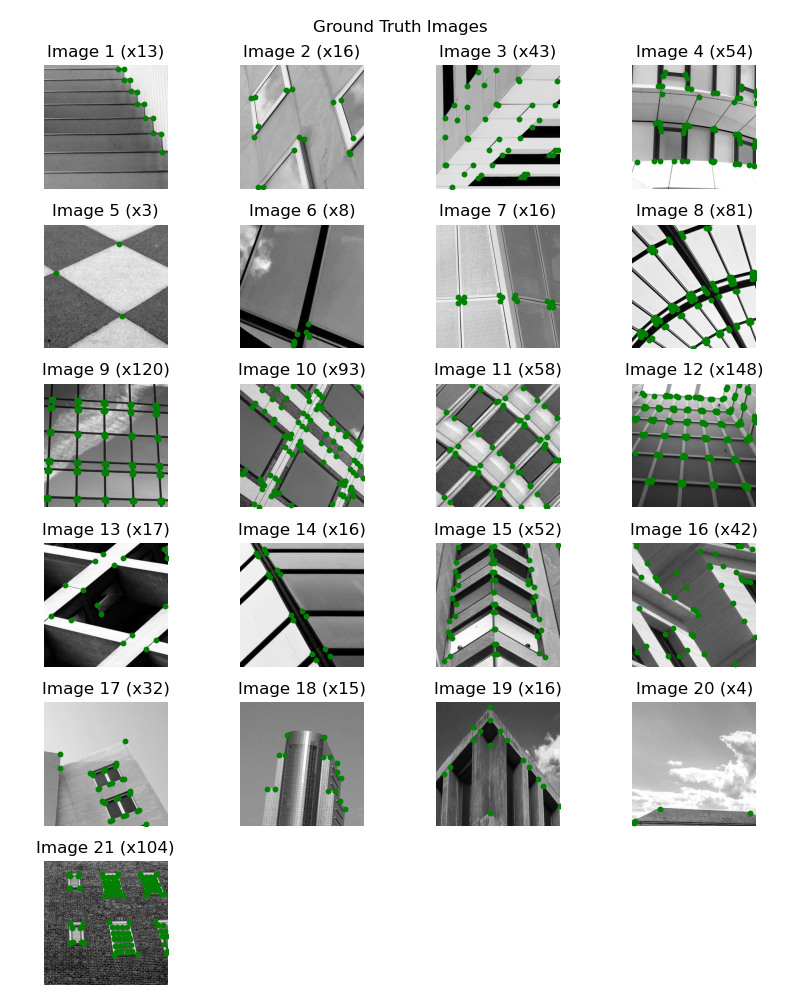
\includegraphics[width=\linewidth]{../results/ground_truth.png}
    \caption{Urban dataset with ground truth corners applied.}
    \label{fig:ground_truth}
    \end{minipage}
    }
\end{figure}
% \twocolumn

\section{Implementation}
\label{section:implementation}

The implementation of the corner detection benchmarking framework was developed in Python, leveraging the OpenCV library for algorithm execution and NumPy for numerical computations. The codebase is organized into modular scripts: \texttt{final\_project.py} orchestrates the benchmarking process, \texttt{parameters.py} defines algorithm parameters and configurations, \texttt{corner\_methods.py} implements the corner detection algorithms, \texttt{utilities.py} provides helper functions for metrics and visualization, and \texttt{distributions.py} handles parameter sampling distributions. This section details the logic flows for data loading, parameter optimization, scale invariance testing, and result generation, highlighting the design choices that ensure robustness and efficiency.\\

\subsection{Data Loading and Preprocessing}
The benchmarking process starts with loading the Urban Corner Datasets, which consist of grayscale images and corresponding ground truth corner annotations stored as text files \cite{Urban_Corner_Dataset}. The \texttt{get\_ground\_truth} function in \texttt{final\_project.py} reads images from a specified directory and their associated corner coordinates from text files, ensuring consistent ordering by sorting filenames numerically based on embedded indices. Each image is loaded in grayscale using \texttt{cv2.imread}, and ground truth corners are parsed into NumPy arrays of (x, y) coordinates. The function also generates a visualization of the ground truth corners overlaid on the images, saved as \texttt{ground\_truth.png} in the output directory, using the \texttt{plot\_ground\_truth} utility from \texttt{utilities.py}. This visualization aids in verifying the dataset integrity. The algorithms are evaluated on raw grayscale inputs. The images and ground truth corners are stored in lists, with corresponding image names extracted from filenames, facilitating subsequent processing and result organization.\\

\subsection{Parameter Optimization}
Parameter optimization is a core component of the benchmarking framework, aiming to find the best parameter settings for each algorithm to maximize performance across multiple metrics. The \texttt{optimize\_across\_images} function in \texttt{final\_project.py} implements a grid search over parameter combinations, evaluating each combination’s performance on all images. The parameter grids are defined in \texttt{parameters.py} using custom distribution classes (\texttt{UniformDist}, \texttt{NormalDist}, \texttt{CategoricalDist}) from \texttt{distributions.py}, which allow flexible sampling of continuous, integer, and categorical parameters.\\

The optimization process starts by sampling parameter values using the \texttt{sample\_param\_grid} function, which generates \texttt{N\_SAMPLES} values for each parameter based on its distribution. For example, the Harris algorithm’s \texttt{ksize} is sampled from a \texttt{CategoricalDist} with options [3, 5, 7, 9, 11] to ensure valid odd integers, while \texttt{k} is sampled from a \texttt{UniformDist} over [0.01, 0.15]. The total number of combinations is computed as the product of the number of unique sampled values for each parameter. The implementation limits the number of evaluated combinations to \texttt{MAX\_SAMPLES} (set to 250) by randomly sampling from the Cartesian product of parameter values using Python's \texttt{random.sample}, see full implementation in Appendix \ref{app:code} for \texttt{distributions.py}.\\

\begin{lstlisting}[style=python, caption={Distributions Example}, label={lst:uniform_dist}]
class UniformDist:
def __init__(self, min_val, max_val, is_int=False):
    self.min_val = min_val
    self.max_val = max_val
    self.is_int = is_int

def sample(self, n_samples):
    samples = np.round(np.random.uniform(self.min_val, self.max_val, n_samples), 4)
    if self.is_int:
        samples = np.round(samples).astype(int)
        samples = np.clip(samples, self.min_val, self.max_val)
        
    return np.unique(samples)[:n_samples]  # Ensure unique samples

    def sample_param_grid(param_grid, n_samples):

sampled_grid = {}
for param_name, dist in param_grid.items():
    sampled_grid[param_name] = dist.sample(n_samples)
return list(sampled_grid.keys()), list(sampled_grid.values())

PARAM_GRIDS = {
    'Harris': {
        'blockSize': UniformDist(min_val=2, max_val=11, is_int=True),
        'ksize': CategoricalDist(options=[3, 5, 7, 9, 11]),  # Only odd integers
        'k': UniformDist(min_val=0.01, max_val=0.15),
        'borderType': CategoricalDist(options=[
            cv2.BORDER_DEFAULT, cv2.BORDER_CONSTANT, cv2.BORDER_REFLECT
        ])
    }
    ... CONTINUED
}
\end{lstlisting}

For each parameter combination, the algorithm is applied to all images, and performance metrics (precision, recall, repeatability, F-score, APR, localization error, corner quantity, and corner quantityS ratio) are computed using \texttt{calculate\_metrics} from \texttt{utilities.py}, reference \cref{lst:optimize_across_images}. The \texttt{calculate\_metrics} function computes the metrics by comparing predicted corners to ground truth corners within a threshold distance (default 5 pixels). True positives (TP), false positives (FP), and false negatives (FN) are determined using pairwise distance computations via \texttt{scipy.spatial.distance.cdist}, enabling precise evaluation of detection accuracy. A final useful metric was developed, corner quantity ratio, defined as \( \frac{1}{|\text{pred} - \text{gt}| + 1} \), which deals with essentially scoring the corner quantity against the ground truth quantity, normalized between 0 and 1.\\

\begin{lstlisting}[style=python, caption={Metric Calculations}, label={lst:optimize_across_images}]
def calculate_metrics(pred_corners, gt_corners, threshold=5.0):
    gt = np.array(gt_corners, dtype=np.float32)
    pred = np.array(pred_corners, dtype=np.float32)

    if pred.ndim == 1 and pred.shape[0] == 2:
        pred = pred.reshape(1, 2)
    if pred.ndim == 1 or pred.size == 0:
        pred = np.empty((0, 2), dtype=np.float32)

    if gt.ndim == 1 and gt.shape[0] == 2:
        gt = gt.reshape(1, 2)
    if gt.ndim == 1 or gt.size == 0:
        gt = np.empty((0, 2), dtype=np.float32)

    corner_quantity = len(pred)
    corner_quantity_ratio = 1 / (np.abs(len(pred) - len(gt_corners)) + 1) ## 1/(|gt - pred| + 1)

    if len(gt) == 0 or len(pred) == 0:
        return 0.0, 0.0, 0.0, 0.0, 0.0, 0.0, corner_quantity, corner_quantity_ratio

    dists = cdist(gt, pred)  
    matched_gt = np.any(dists <= threshold, axis=1)
    matched_pred = np.any(dists <= threshold, axis=0)

    TP = np.sum(matched_gt)
    FP = len(pred) - np.sum(matched_pred)
    FN = len(gt) - TP

    precision = TP / (TP + FP) if (TP + FP) > 0 else 0
    recall = TP / (TP + FN) if (TP + FN) > 0 else 0
    repeatability = TP / len(gt) if len(gt) > 0 else 0

    denom = (precision + recall)
    f_score = 2 * (precision * recall) / denom if denom > 0 else 0
    apr = (precision + recall) / 2  # Arithmetic Mean 

    localization_error = 0.0
    if TP > 0:
        min_dists = np.min(dists, axis=1) 
        matched_dists = min_dists[matched_gt] 
        localization_error = np.mean(matched_dists) if len(matched_dists) > 0 else 0.0

    return precision, recall, repeatability, f_score, apr, localization_error, corner_quantity, corner_quantity_ratio
\end{lstlisting}

The metrics are aggregated by averaging across images, with speed and localization error normalized to [0, 1] (inverted to favor lower values). A composite score is calculated as a weighted sum of selected metrics (defined by \texttt{vars} and \texttt{weights} (or can be), see reference \cref{{lst:scoring}}), allowing flexible prioritization of performance aspects. The combination yielding the highest score is retained as the optimal parameter set. The scoring metrics used in the overall score proved difficult to determine. Further discussion on scoring is found in Section \ref{section:results}.\\

\begin{lstlisting}[style=python, caption={Best Combination Scoring}, label={lst:scoring}]
    avg_speed = np.mean(normalized_speeds)
    avg_precision = np.mean(precisions)
    avg_recall = np.mean(recalls)
    avg_le = np.mean(normalized_le)
    avg_corner_quant_ratios = np.mean(corner_quantity_ratios)
    vars = np.array([avg_speed, avg_precision, avg_recall, avg_le, avg_corner_quant_ratios])
    score = np.sum(vars) / len(vars)
\end{lstlisting}

\subsection{Corner Detection Algorithms}
The corner detection algorithms are implemented in \texttt{corner\_methods.py}, wrapping OpenCV’s implementations to standardize input/output formats. Each function accepts a grayscale image and an optional dictionary of parameters, returning corner coordinates as a NumPy array of (x, y) floats. The Harris detector uses \texttt{cv2.cornerHarris} with post-processing to select strong corners via dilation and thresholding. Shi-Tomasi employs \texttt{cv2.goodFeaturesToTrack}, while FAST, ORB, SIFT, BRISK, AGAST, KAZE, and AKAZE use their respective OpenCV feature detectors (\texttt{cv2.FastFeatureDetector}, \texttt{cv2.ORB}, etc.). Default parameters are provided to ensure functionality when no parameters are specified, but the optimization process overrides these with sampled values.\\


\begin{lstlisting}[style=python, caption={Corner Detection Wrapper Implementations}, label={lst:corern_methods}]
def harris(image, args=None):
    args = args or {'blockSize': 2, 'ksize': 3, 'k': 0.04}
    corners = cv2.cornerHarris(image, **args)
    corners = cv2.dilate(corners, None)
    corners = np.column_stack(np.where(corners > 0.01 * corners.max()))
    return corners[:, ::-1].astype(np.float32)

def shi_tomasi(image, args=None):
    args = args or {'maxCorners': 25, 'qualityLevel': 0.01, 'minDistance': 10}
    corners = cv2.goodFeaturesToTrack(image, **args)
    return corners[:, 0].astype(np.float32) if corners is not None else np.array([])

def fast(image, args=None):
    args = args or {'threshold': 25, 'type': cv2.FAST_FEATURE_DETECTOR_TYPE_7_12}
    fast = cv2.FastFeatureDetector_create(**args)
    keypoints = fast.detect(image, None)
    return np.array([kp.pt for kp in keypoints], dtype=np.float32)

... CONTINUED
\end{lstlisting}

The modular design allows easy extension to additional algorithms, with each function handling algorithm-specific parameter requirements. For instance, Harris includes \texttt{borderType} to support different boundary handling options, while ORB includes parameters like \texttt{nfeatures} and \texttt{scaleFactor} to control keypoint detection. A large decision in this project was made to only record locations of corners (or keypoints) detected by the algorithms, thought some will provide more information called desciptors (as an example). \\

\subsection{Scale Invariance Testing}
Scale invariance is evaluated using the \texttt{test\_scale\_invariance} function in \texttt{final\_project.py}, which tests each algorithm’s performance across multiple image scales. The \texttt{create\_scaled\_images} utility generates scaled versions of each image using \texttt{cv2.resize} with scales defined in \texttt{SCALES} ([0.25, 1.0, 4.0]). For each algorithm, the optimal parameters from the optimization phase are used to detect corners on scaled images, and metrics are computed by comparing detected corners to scaled ground truth corners.\\

Scale invariance is quantified as \( 1 - \text{CV} \), where CV is the coefficient of variation (standard deviation divided by mean) of repeatability across scales. A higher score indicates better consistency in corner detection across scales. The function also generates visualizations for a randomly selected image, plotting detected and ground truth corners at each scale, saved in the \texttt{scale\_invariance\_samples} directory. The plots, produced by \texttt{generate\_scale\_invariance\_samples}, provide qualitative insights into scale robustness.\\

\subsection{Result Generation and Visualization}
The benchmarking results are aggregated and visualized to help with analysis. The \texttt{run\_benchmarking} function orchestrates the optimization and evaluation, storing results in dictionaries for aggregated metrics (\texttt{results}), individual image metrics (\texttt{individual\_results}), and all parameter combination metrics (\texttt{all\_metrics\_per\_algorithm}). Results are saved as NumPy archives (\texttt{.npz}) for each algorithm and image, enabling post-processing for the data.\\

Several visualization functions were written in \texttt{utilities.py} to generate outputs:
\begin{itemize}
    \item \texttt{generate\_sample\_detections}: Produces sample detection images for each algorithm on a random image, showing ground truth (green circles) and detected corners (red circles).
    \item \texttt{generate\_comparison\_tables}: Creates a LaTeX table summarizing mean metrics across algorithms, saved as \texttt{comparison\_table.txt}.
    \item \texttt{generate\_param\_report}: Generates a LaTeX table of optimal parameters, total combinations tested, and best scores, saved as \texttt{optimal\_parameters.txt}.
    \item \texttt{visualize\_results}: Plots metrics across images for all algorithms, saved as \texttt{benchmark\_results.png}.
    \item \texttt{plot\_best\_combination}: Plots metrics for the best parameter combination per algorithm, saved in \texttt{best\_combination\_plots}.
    \item \texttt{plot\_all\_combinations}: Visualizes all parameter combinations’ metrics, highlighting the best combination, saved in \texttt{all\_combinations\_plots}.
    \item \texttt{plot\_scale\_invariance}: Plots metrics across scales for each image, saved in \texttt{scale\_invariance\_plots}.
    \item \texttt{plot\_all\_detections}: Plots all test images with all detected corners according to the optimimally found variable combinations.
    \item 
\end{itemize}

The implementation is extensible via the use of a configuration file \texttt{parameters.py} allowing additional algorithms or metrics to be integrated by modifying \texttt{ALGORITHMS} and \texttt{PARAM\_GRIDS} in \texttt{parameters.py}. The use of random seeding (\texttt{SEED = 11001}) ensures reproducibility, and the modular structure facilitates debugging and maintenance.\\

\subsection{Troubleshooting and Challenges}
This implementation was written from entirely scratch and provides a comprehensive framework for benchmarking corner detection algorithms, balancing computational efficiency with evaluation. The generated visualizations and tables shown in the next section enable detailed analysis would often take hours to run, due to the quantity of corners detected (the plotting scripts may not be well optimized.). One large challenge was also figuring out how to get each method to spit out corners. Additionally, there was difficulty with combining metrics to determine the best overall combination of parameter used in each algorithm. Different seed numbers also caused problems, with occasionally throwing errors in the CV2 functions. Setting up a framework to run on a scale greater than what is presented here requires much more polishing, in addition to robust error handling. It should be noted again that each of these algorithms have their own design use cases, and by only using the locations of corners provided, by the algorithms (some return more than just locations), the algorithms are not all being used to their fullest extent.\\

Several days were spent trying to optimize the results according to what made sense for this project. The fact stands that corner detection performance is subjective to the application (or user). These algorithms overall are doing their intended jobs at attempting to find corners in an image. After much thought and experimentation, many of these algorithms could be used alongside a filter of some sort (nonmaxSuppression is good) to reduce quanityt of points generated. Harris would greatly benefit from that, while FAST has it baked in with an option. The challenge is fairly assessing each algorithm, knowing some are simply built with other purposes in mind.\\

In order to score these algorithms fairly, a metric was developed that would penalize deviations from the ground truth corner count, contributing to the robustness assessment. That metric is the corner quantity ratio mentioned in Section \ref{section:implementation}. Is is specifcally created to combine with the inverted Speed, Precision, Recall, and the localization error. Over or under prediciting corners should be penalized, this metric allows for this, and once this was thrown in the scoring metric, the best candidate for each algorithm seemed to show visually much better results overall.

\section{Results}
\label{section:results}

The benchmarking results for the nine corner detection algorithms (Harris, Shi-Tomasi, FAST, ORB, SIFT, BRISK, AGAST, KAZE, and AKAZE) are presented in three categories: individual image performance, aggregate performance across all images, and scale invariance performance. Evaluations were conducted on the Urban Corner Datasets \cite{Urban_Corner_Dataset}, measuring precision, recall, repeatability, F-score, arithmetic mean of precision and recall (APR), localization error, corner quantity, corner quantity ratio, and execution time (speed). Visualizations and tables, generated by the implemented framework, provide detailed insights into each algorithm’s perfo\\rmance, with optimal parameters derived from the grid search described in Section \ref{section:implementation}.

\subsection{Individual Image Results}
Individual image results reveal how each algorithm performs on specific images from the Urban Corner Datasets, capturing variability due to factors like lighting, texture, and corner density. The \texttt{plot\_best\_combination} function produced plots showing metric values for the optimal parameter set across all images for each algorithm. Figures \ref{fig:harris_combinations} through \ref{fig:fast_combinations} illustrate the performance of the three different algorithms, displaying metrics such as precision, recall, and speed across each benchmark images.\\

Qualitative insights are provided by sample detection images generated by \texttt{generate\_sample\_detections}. Reference \cref{fig:sample_detection_harris} through \cref{fig:sample_detection_fast}, which show detected corners (red circles) and ground truth corners (green circles) for a randomly selected image using optimized parameters (\cref{tab:optimal_parameters}), highlighting ability to closely match ground truth corners. These results emphasize the need for parameter optimization, as suboptimal settings significantly degraded performance. It is clear that performance is noisy.\\

Note: A full series of test images for each algorithm are shown in Appendix \ref{app:optimization_results}.

\begin{figure}
    \centering
    \fbox{
        \begin{minipage}{0.4\textwidth}
    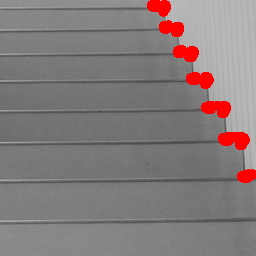
\includegraphics[width=\linewidth]{../results/sample_detections/Harris_detected.png}
    \caption{Sample detection for Harris on a randomly selected image, with ground truth corners (green circles) and detected corners (red circles).}
    \label{fig:sample_detection_harris}
    \end{minipage}
    }
\end{figure}

\begin{figure}
    \centering
    \fbox{
        \begin{minipage}{0.4\textwidth}
    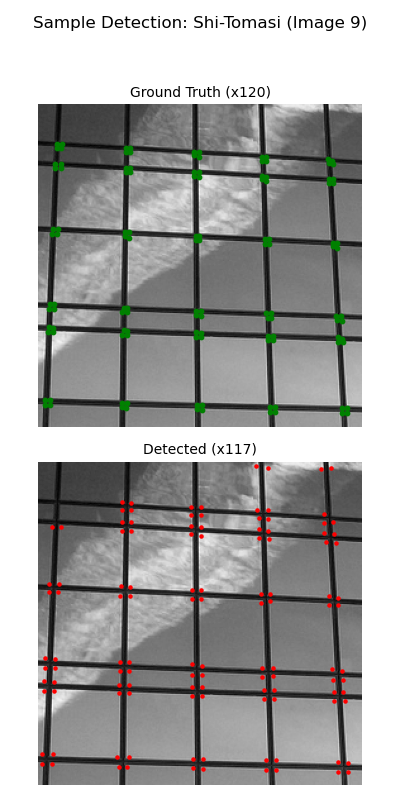
\includegraphics[width=\linewidth]{../results/sample_detections/Shi-Tomasi_detected.png}
    \caption{Sample detection for Shi-Tomasi on a randomly selected image, with ground truth corners (green circles) and detected corners (red circles).}
    \label{fig:sample_detection_shi}
    \end{minipage}
    }
\end{figure}

\begin{figure}
    \centering
    \fbox{
        \begin{minipage}{0.4\textwidth}
    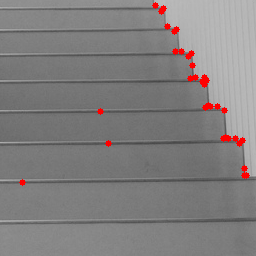
\includegraphics[width=\linewidth]{../results/sample_detections/FAST_detected.png}
    \caption{Sample detection for FAST on a randomly selected image, with ground truth corners (green circles) and detected corners (red circles).}
    \label{fig:sample_detection_fast}
    \end{minipage}
    }
\end{figure}

\begin{figure}
    \centering
    \fbox{
        \begin{minipage}{0.47\textwidth}
    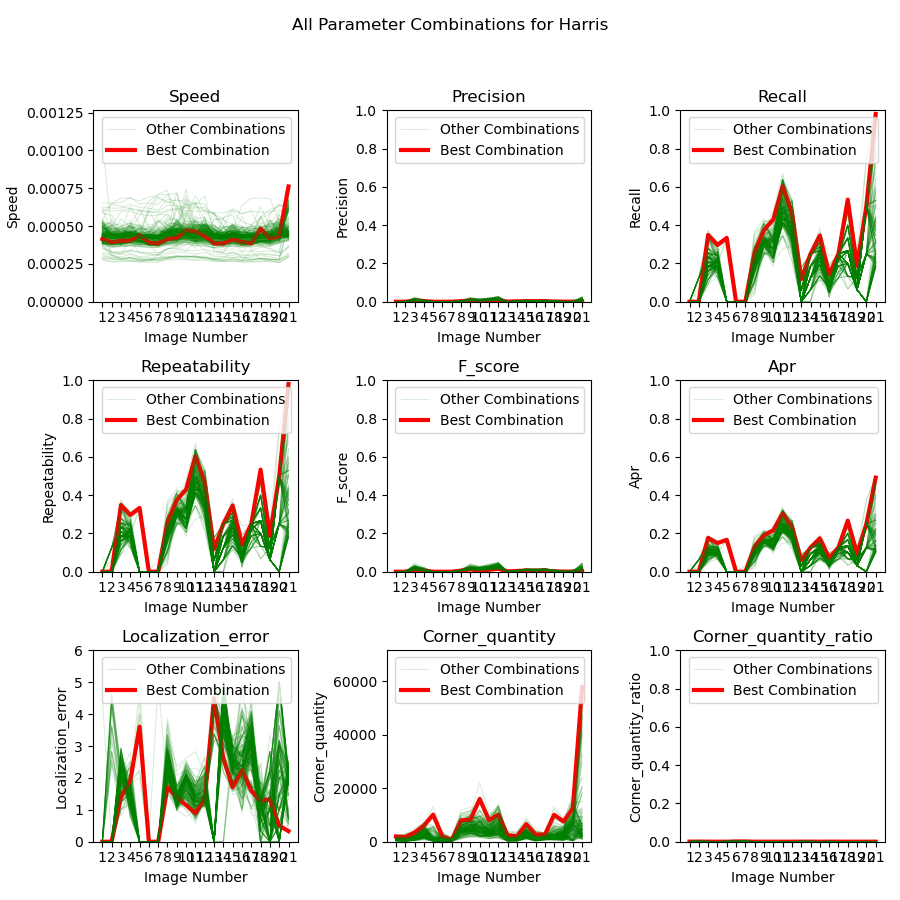
\includegraphics[width=\linewidth]{../results/all_combinations_plots/Harris_all_combinations.png}
    \caption{Best parameter combination metrics for the Harris algorithm across individual images, showing precision, recall, repeatability, F-score, APR, localization error, corner quantity, corner quantity ratio, and speed.}
    \label{fig:harris_combinations}
    \end{minipage}
    }
\end{figure}

\begin{figure}
    \centering
    \fbox{
        \begin{minipage}{0.47\textwidth}
    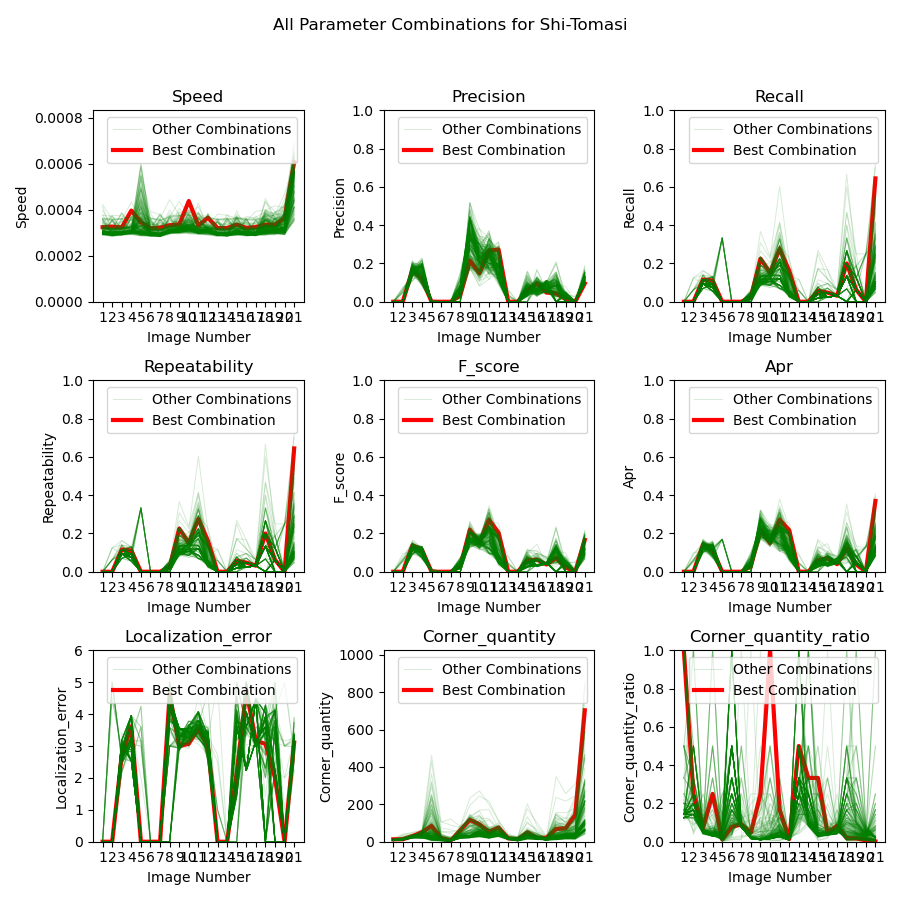
\includegraphics[width=\linewidth]{../results/all_combinations_plots/Shi-Tomasi_all_combinations.png}
    \caption{Best parameter combination metrics for the Shi-Tomasi algorithm across individual images, showing precision, recall, repeatability, F-score, APR, localization error, corner quantity, corner quantity ratio, and speed.}
    \label{fig:shi_tomasi_combinations}
    \end{minipage}
    }
\end{figure}

\begin{figure}
    \centering
    \fbox{
        \begin{minipage}{0.47\textwidth}
    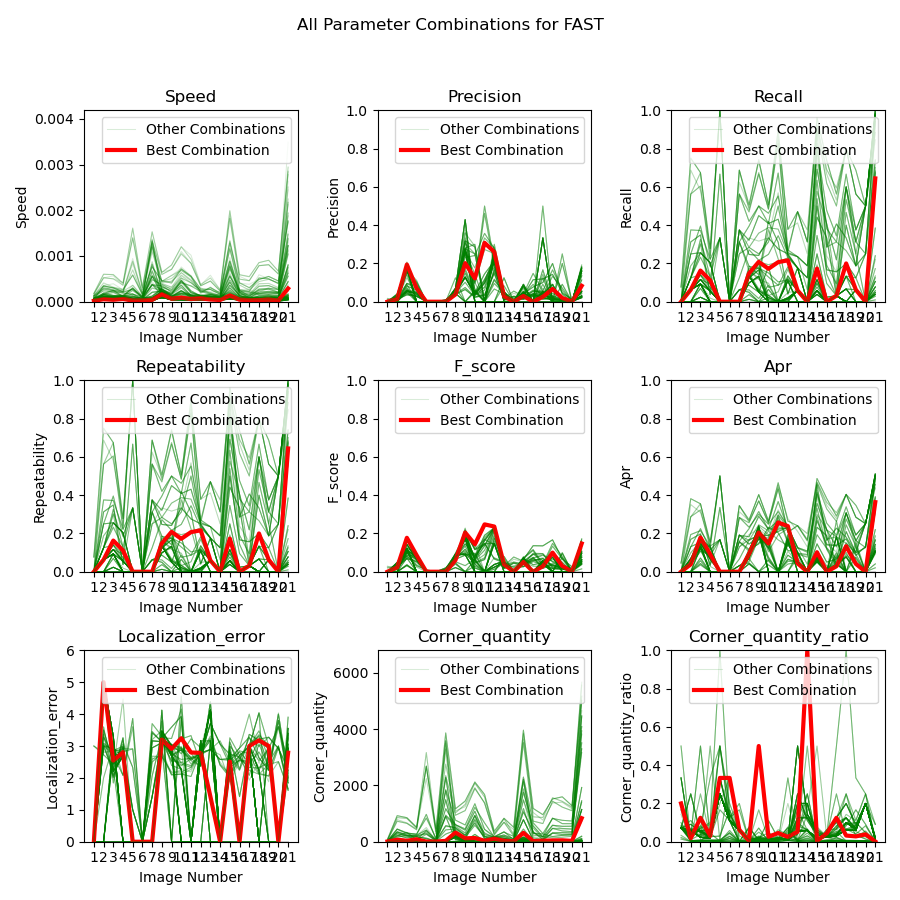
\includegraphics[width=\linewidth]{../results/all_combinations_plots/FAST_all_combinations.png}
    \caption{Best parameter combination metrics for the FAST algorithm across individual images, showing precision, recall, repeatability, F-score, APR, localization error, corner quantity, corner quantity ratio, and speed.}
    \label{fig:fast_combinations}
    \end{minipage}
    }
\end{figure}

\begin{table}
    \centering
    \fbox{
        \begin{minipage}{0.47\textwidth}
    \small
    \caption{Optimal Parameters for Detection Algorithms}
    \label{tab:optimal_parameters}
    \begin{tabular}{lp{3cm}cc}
    \toprule
    \textbf{Algorithm} & \textbf{Optimal Parameters} & \textbf{$\#$ Tests} & \textbf{Best Score} \\
    \midrule
    \multirow{4}{*}{Harris} & \multirow{4}{*}{\parbox{3.25cm}{\raggedright blockSize: 9\\ksize: 3\\k: 0.0118\\borderType: 0}} & \multirow{4}{*}{250}  & \multirow{4}{*}{0.3053} \\
    & & \\
    & & \\
    & & \\
    & & \\
    & & \\
    \multirow{4}{*}{Shi-Tomasi} & \multirow{4}{*}{\parbox{3.25cm}{\raggedright maxCorners: 266\\qualityLevel: 0.0907\\minDistance: 29\\blockSize: 9}} & \multirow{4}{*}{250}  & \multirow{4}{*}{0.3317} \\
    & & \\
    & & \\
    & & \\
    & & \\
    & & \\
    \multirow{2}{*}{FAST} & \multirow{2}{*}{\parbox{3.25cm}{\raggedright threshold: 48\\type: 2}} & \multirow{2}{*}{250}  & \multirow{2}{*}{0.3408} \\
    & & \\
    & & \\
    & & \\
    \multirow{6}{*}{ORB} & \multirow{6}{*}{\parbox{3.25cm}{\raggedright nfeatures: 4236\\scaleFactor: 1.3362\\nlevels: 4\\edgeThreshold: 36\\patchSize: 37\\fastThreshold: 12}} & \multirow{6}{*}{250}  & \multirow{6}{*}{0.3224} \\
    & & \\
    & & \\
    & & \\
    & & \\
    & & \\
    & & \\
    & & \\
    \multirow{4}{*}{SIFT} & \multirow{4}{*}{\parbox{3.25cm}{\raggedright nOctaveLayers: 2\\contrastThreshold: 0.1349\\edgeThreshold: 26\\sigma: 1.8144}} & \multirow{4}{*}{250}  & \multirow{4}{*}{0.3497} \\
    & & \\
    & & \\
    & & \\
    & & \\
    & & \\
    \multirow{3}{*}{BRISK} & \multirow{3}{*}{\parbox{3.25cm}{\raggedright thresh: 12\\octaves: 4\\patternScale: 0.5133}} & \multirow{3}{*}{250}  & \multirow{3}{*}{0.2822} \\
    & & \\
    & & \\
    & & \\
    & & \\
    \multirow{2}{*}{AGAST} & \multirow{2}{*}{\parbox{3.25cm}{\raggedright threshold: 33\\type: 0}} & \multirow{2}{*}{250}  & \multirow{2}{*}{0.3564} \\
    & & \\
    & & \\
    & & \\
    \multirow{4}{*}{KAZE} & \multirow{4}{*}{\parbox{3.25cm}{\raggedright threshold: 0.0029\\nOctaves: 2\\nOctaveLayers: 4\\diffusivity: 1}} & \multirow{4}{*}{250}  & \multirow{4}{*}{0.3083} \\
    & & \\
    & & \\
    & & \\
    & & \\
    & & \\
    \multirow{4}{*}{AKAZE} & \multirow{4}{*}{\parbox{3.25cm}{\raggedright threshold: 0.0011\\nOctaves: 3\\nOctaveLayers: 3\\diffusivity: 0}} & \multirow{4}{*}{250}  & \multirow{4}{*}{0.3361} \\
    & & \\
    & & \\
    & & \\
    & & \\
    & & \\
    \bottomrule
    \end{tabular}
\end{minipage}
}
\end{table}

\subsection{Aggregate Results}
Aggregate results provide a comprehensive comparison by averaging metrics across all images. The \texttt{generate\_comparison\_tables} function created a LaTeX table, included as Table \ref{tab:comparison_table}, summarizing mean precision, recall, repeatability, speed, F-score, APR, localization error, and corner quantity ratio for each algorithm. Figure \ref{fig:benchmark_results} compares aggregate metrics across all algorithms, generated by \texttt{visualize\_results}.\\

Table~\ref{tab:comparison_table} presents the aggregate benchmarking results across all algorithms. ???? and ???? demonstrated the fastest execution times, both achieving mean speeds below ???? seconds per image, confirming their suitability for real-time applications. In contrast, ???? and ???? exhibited significantly slower performance, with execution times above about ???? seconds, attributable to their scale-space constructions. Precision and recall values varied notably across methods. BRISK achieved the highest recall (0.439) but suffered from extremely low precision (????), indicating a tendency to over-detect features. Conversely, ???? achieved the lowest precision (????) despite its moderate repeatability (????). ???? demonstrated the best localization accuracy with a mean localization error of ???? pixels, outperforming all other detectors.

Regarding the corner quantity ratio metric, ???? achieved the highest value (????), suggesting that it produced a number of detected corners most closely matching the ground truth quantity. ????, in contrast, had the lowest corner quantity ratio (????), indicating under-detection.


\begin{figure}[h]
    \centering
    \fbox{
        \begin{minipage}{0.47\textwidth}
    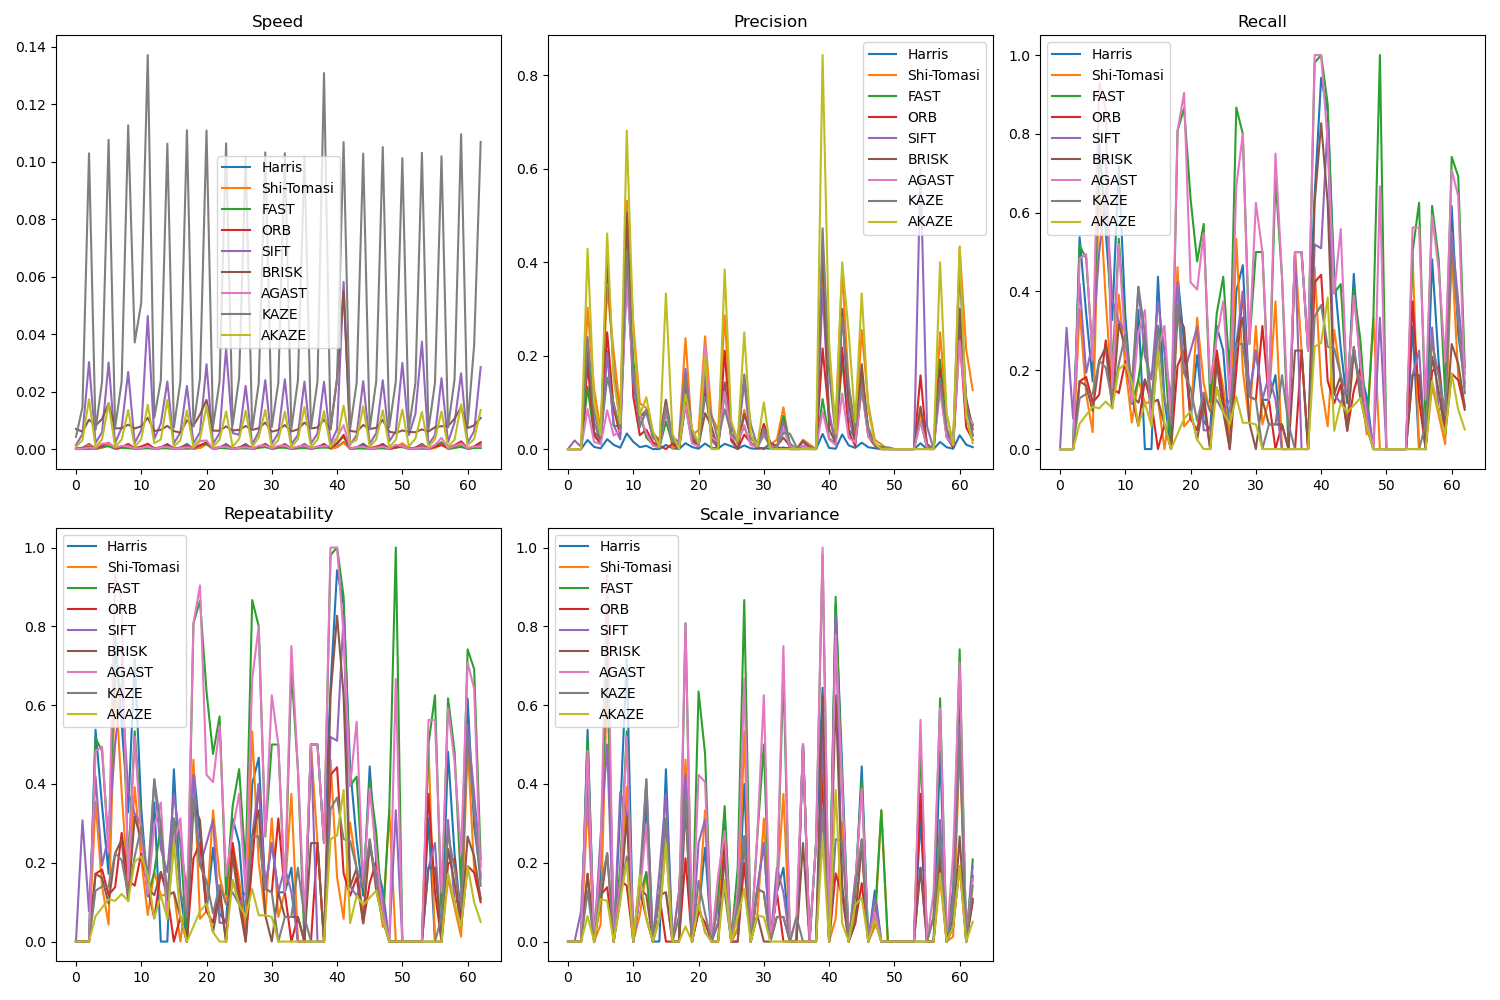
\includegraphics[width=\linewidth]{../results/benchmark_results.png}
    \caption{Aggregate metrics across all images for each algorithm, comparing precision, recall, repeatability, speed, F-score, APR, localization error, corner quantity, and corner quantity ratio.}
    \label{fig:benchmark_results}
    \end{minipage}
    }
\end{figure}

\begin{figure}[h]
    \centering
    \fbox{
        \begin{minipage}{0.47\textwidth}
    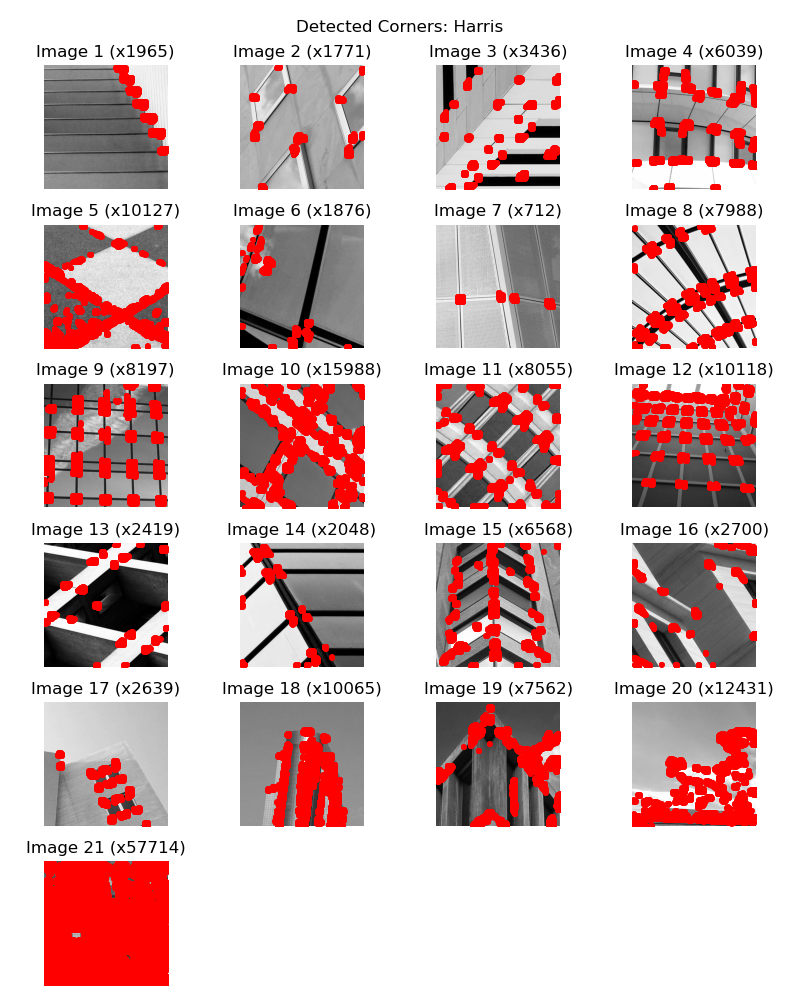
\includegraphics[width=\linewidth]{../results/sample_detections/Harris_all_detections.png}
    \caption{Urban dataset with detected Harris corners applied.}
    \label{fig:harris_all}
    \end{minipage}
    }
\end{figure}

\begin{figure}[h]
    \centering
    \fbox{
        \begin{minipage}{0.47\textwidth}
    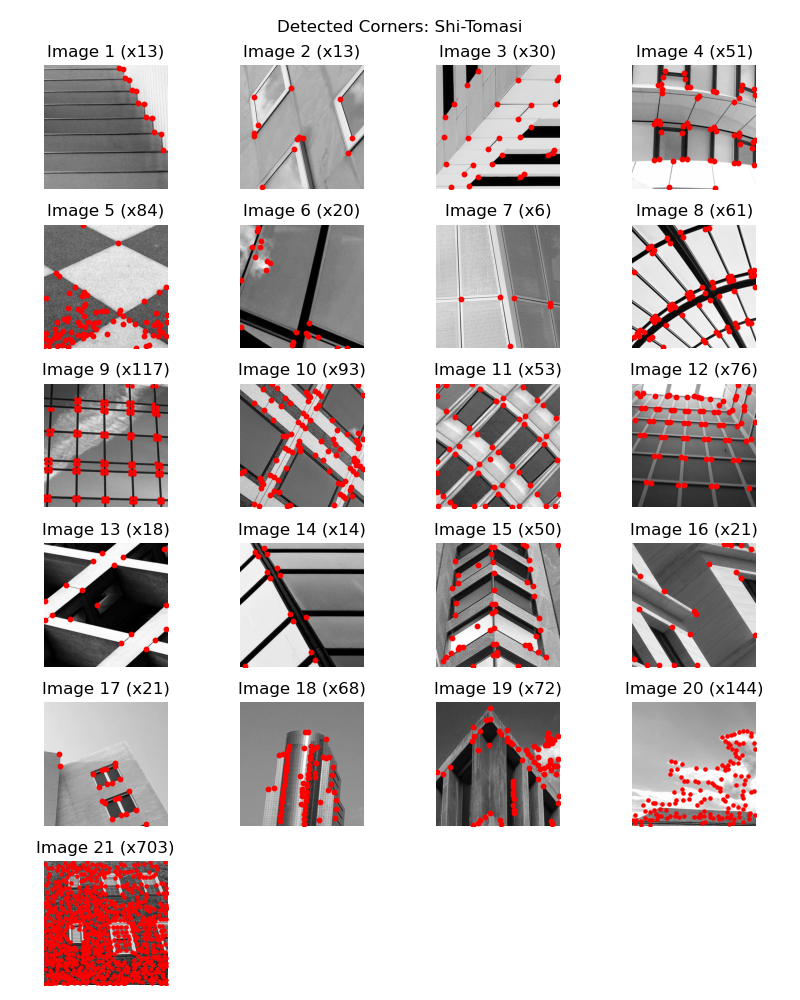
\includegraphics[width=\linewidth]{../results/sample_detections/Shi-Tomasi_all_detections.png}
    \caption{Urban dataset with detected Shi-Tomasi corners applied.}
    \label{fig:shi_all}
    \end{minipage}
    }
\end{figure}

\begin{figure}[h]
    \centering
    \fbox{
        \begin{minipage}{0.47\textwidth}
    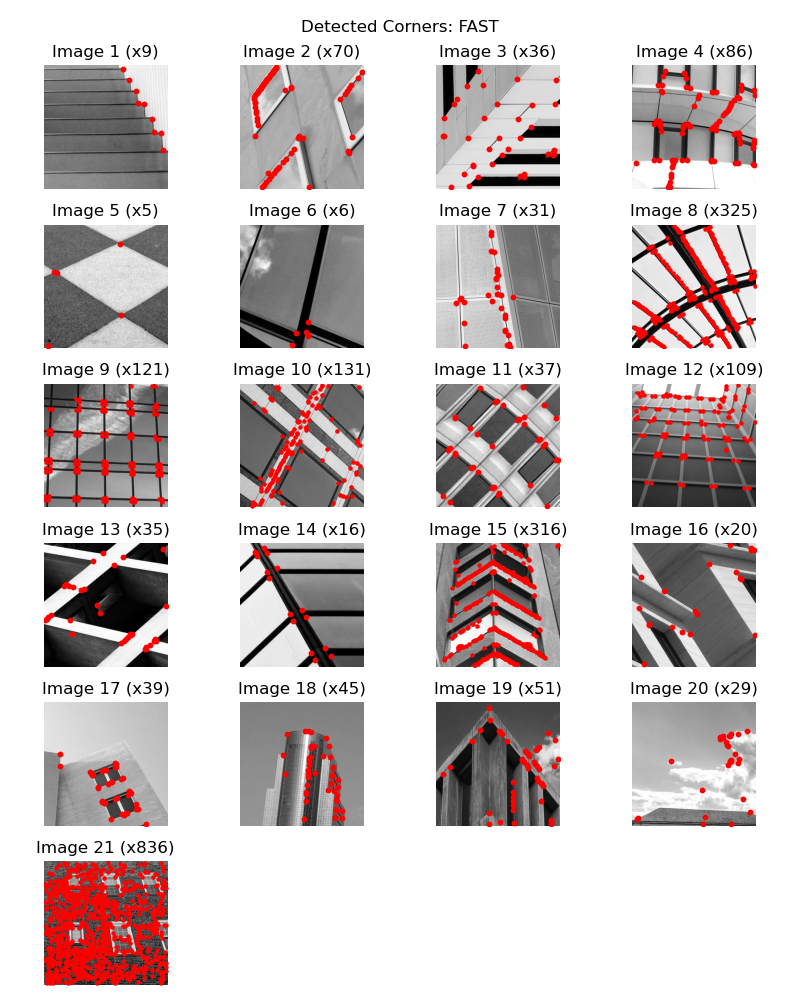
\includegraphics[width=\linewidth]{../results/sample_detections/FAST_all_detections.png}
    \caption{Urban dataset with detected FAST corners applied.}
    \label{fig:shi_all}
    \end{minipage}
    }
\end{figure}

\subsection{Scale Invariance Results}
Scale invariance was assessed by applying each algorithm to images scaled at factors [0.25, 1.0, 4.0] using the \texttt{test\_scale\_invariance} function. The scale invariance score, computed as \( 1 - \text{CV} \) (where CV is the coefficient of variation of repeatability across scales), measures detection consistency. Figures \ref{fig:scale_invariance_harris} through \ref{fig:scale_invariance_fast} show the scale invariance plot for a few algorithms, generated by \texttt{plot\_scale\_invariance}, displaying metrics across scales for each image.\\

Figures \ref{fig:scale_invariance_sample_harris} through \ref{fig:scale_invariance_sample_fast} illustrates a sample image at each scale for Harris, Shi-Tomais, and FAST algorithms, generated by \texttt{generate\_scale\_invariance\_samples}, showing ground truth (green circles) and detected corners (red circles). These images only show a subset of the algorithms and test images.\\

Table \ref{tab:scale_invariance_scores} reports the scale invariance scores. (????) achieved the best scale robustness ((????)), followed by ???? (????) and (????) ((????)). (????) and (????) exhibited the poorest scale invariance, with scores of (????) and (????), respectively, reflecting their design focus on speed over multi-scale robustness.\\

Note: A full series of test images for each algorithm are shown in Appendix \ref{app:scale_invariance_results}. \\

\begin{table}[t]
    \centering
    \fbox{
        \begin{minipage}{0.3\textwidth}
    \small
    \caption{Best Mean Scale Invariance Scores for the Corner Detection Algorithms}
    \label{tab:scale_invariance_scores}
    \begin{tabular}{lc}
    \toprule
    \textbf{Algorithm} & \textbf{Scale Invariance Score} \\
    \midrule
    AGAST & 0.037 \\
    AKAZE & 0.125 \\
    BRISK & 0.443 \\
    FAST & 0.050 \\
    Harris & 0.154 \\
    KAZE & 0.110 \\
    ORB & 0.059 \\
    SIFT & 0.083 \\
    Shi-Tomasi & 0.169 \\
    \bottomrule
    \end{tabular}
\end{minipage}
}
\end{table}

\begin{figure}[h]
    \centering
    \fbox{
        \begin{minipage}{0.45\textwidth}
    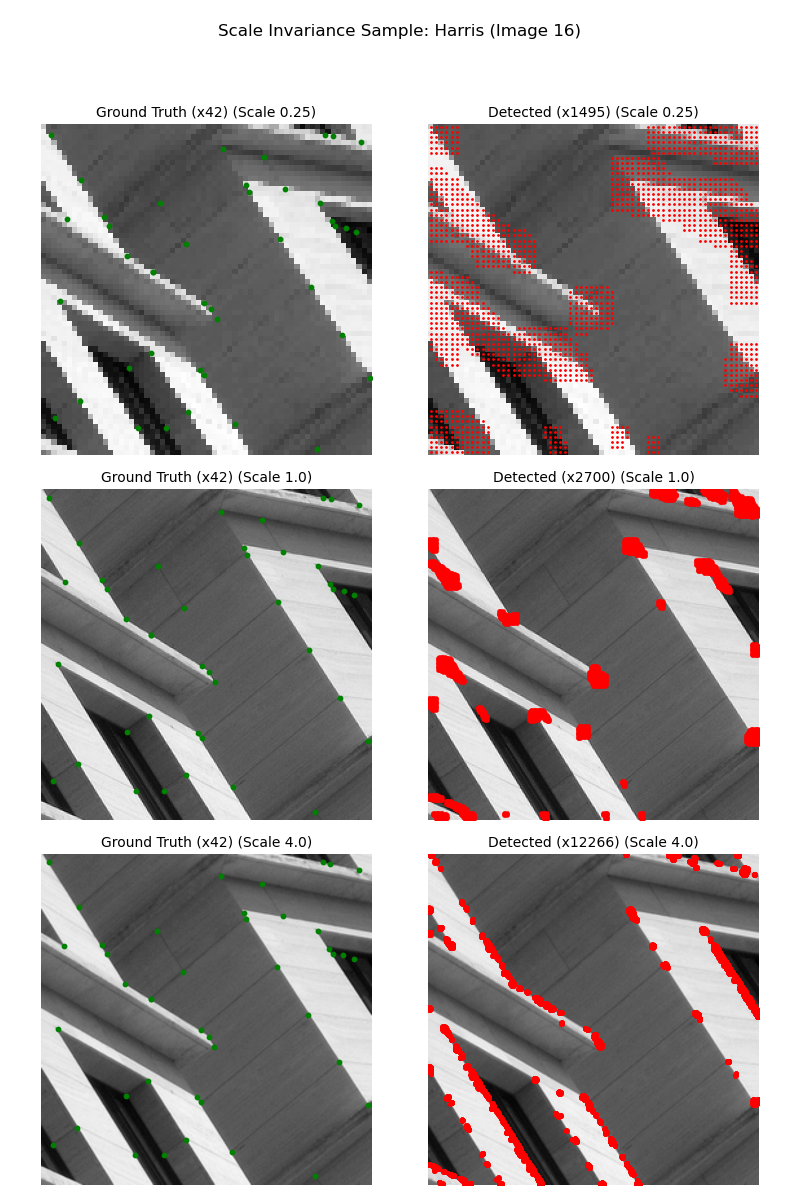
\includegraphics[width=\linewidth]{../results/scale_invariance_samples/Harris_scale_invariance_sample.png}
    \caption{Scale invariance sample for Harris on a randomly selected image, showing ground truth (green circles) and detected corners (red circles) at scales [0.25, 1.0, 4.0].}
    \label{fig:scale_invariance_sample_harris}
    \end{minipage}
    }
\end{figure}

\begin{figure}[h]
    \centering
    \fbox{
        \begin{minipage}{0.45\textwidth}
    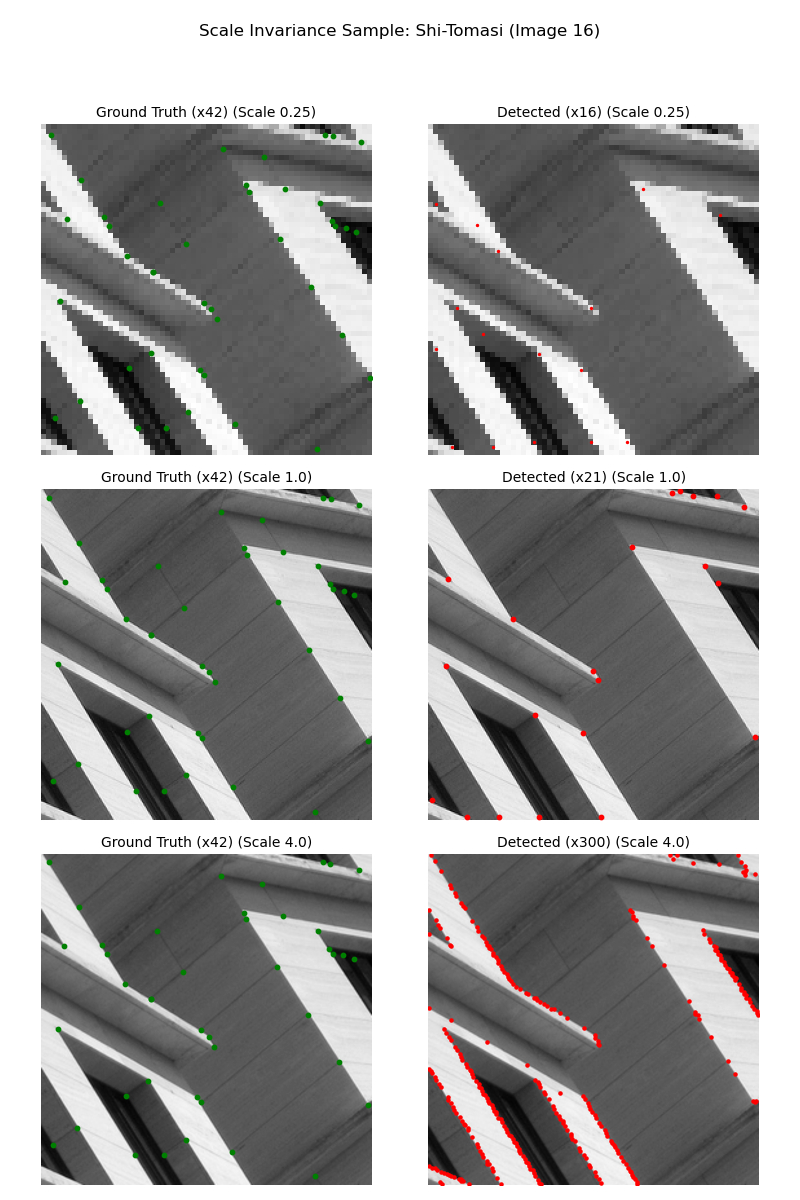
\includegraphics[width=\linewidth]{../results/scale_invariance_samples/Shi-Tomasi_scale_invariance_sample.png}
    \caption{Scale invariance sample for Shi-Tomasi on a randomly selected image, showing ground truth (green circles) and detected corners (red circles) at scales [0.25, 1.0, 4.0].}
    \label{fig:scale_invariance_sample_shi}
    \end{minipage}
    }
\end{figure}

\begin{figure}[h]
    \centering
    \fbox{
        \begin{minipage}{0.45\textwidth}
    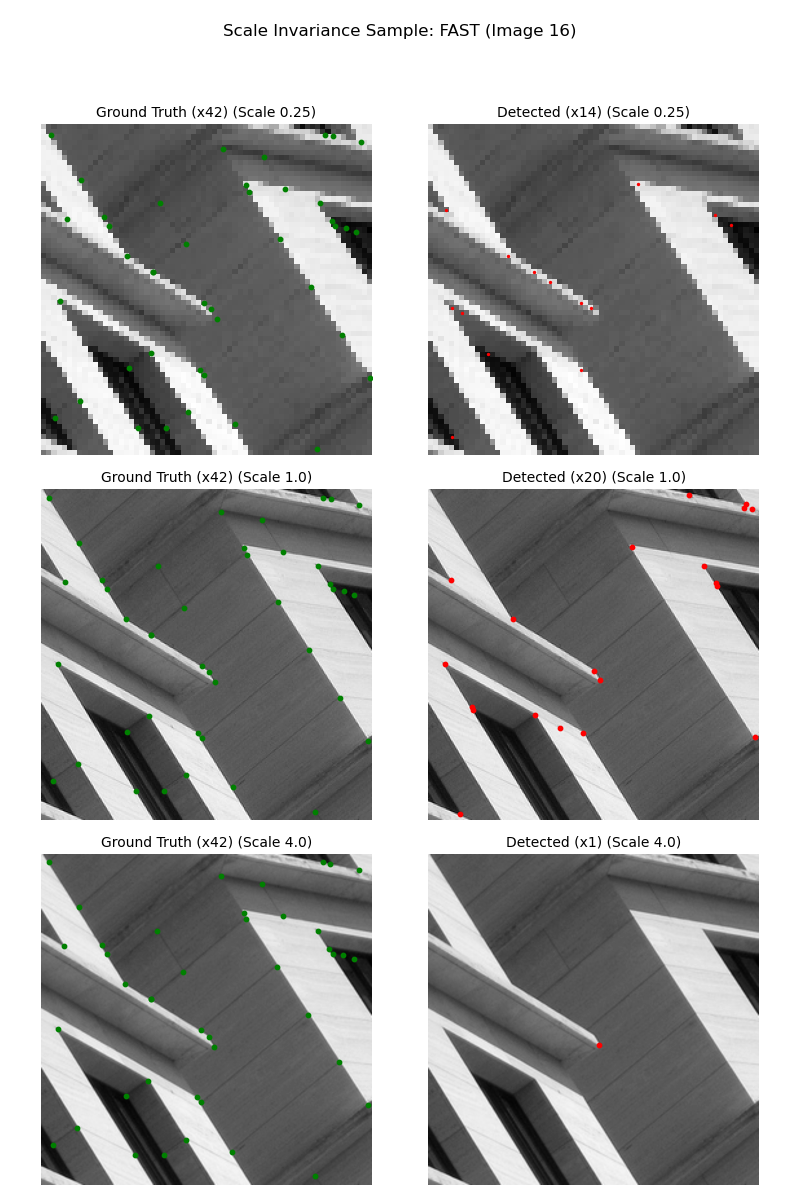
\includegraphics[width=\linewidth]{../results/scale_invariance_samples/FAST_scale_invariance_sample.png}
    \caption{Scale invariance sample for FAST on a randomly selected image, showing ground truth (green circles) and detected corners (red circles) at scales [0.25, 1.0, 4.0].}
    \label{fig:scale_invariance_sample_fast}
    \end{minipage}
    }
\end{figure}

\begin{figure}[h]
    \centering
    \fbox{
        \begin{minipage}{0.47\textwidth}
    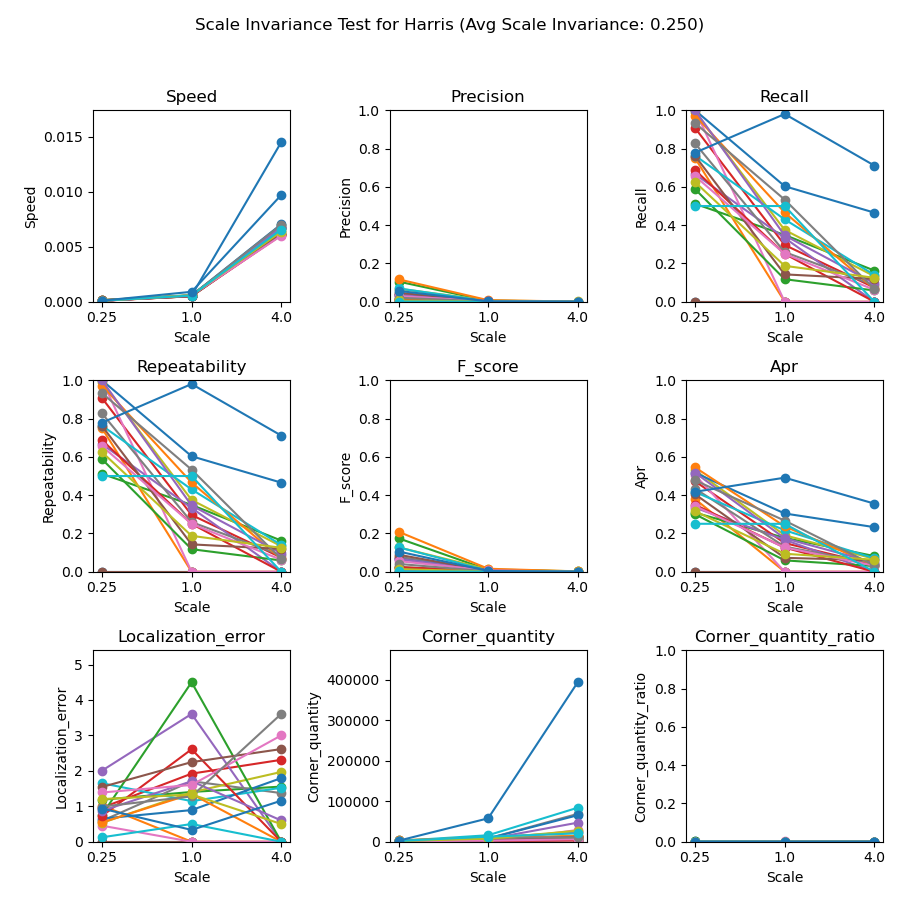
\includegraphics[width=\linewidth]{../results/scale_invariance_plots/Harris_scale_invariance.png}
    \caption{Scale invariance results for Harris, showing metrics across scales [0.25, 1.0, 4.0] for each image, with an average scale invariance score.}
    \label{fig:scale_invariance_harris}
    \end{minipage}
    }
\end{figure}

\begin{figure}[h]
    \centering
    \fbox{
        \begin{minipage}{0.47\textwidth}
    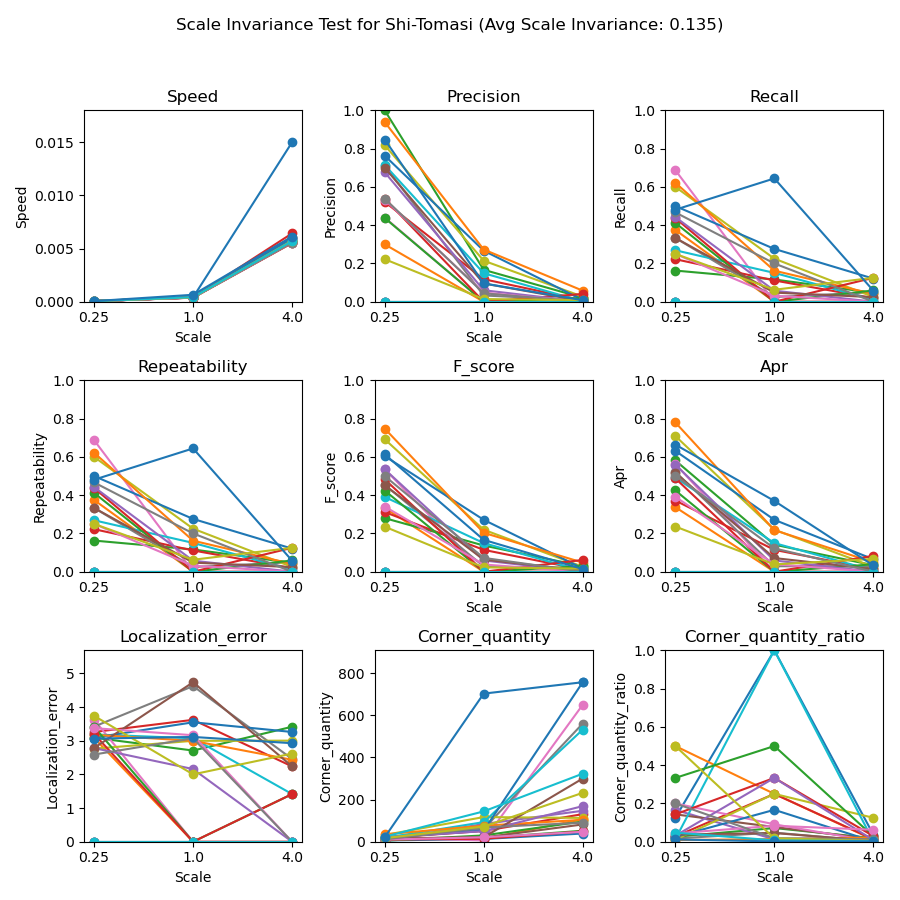
\includegraphics[width=\linewidth]{../results/scale_invariance_plots/Shi-Tomasi_scale_invariance.png}
    \caption{Scale invariance results for Shi-Tomasi, showing metrics across scales [0.25, 1.0, 4.0] for each image, with an average scale invariance score.}
    \label{fig:scale_invariance_shi}
    \end{minipage}
    }
\end{figure}

\begin{figure}[h]
    \centering
    \fbox{
        \begin{minipage}{0.47\textwidth}
    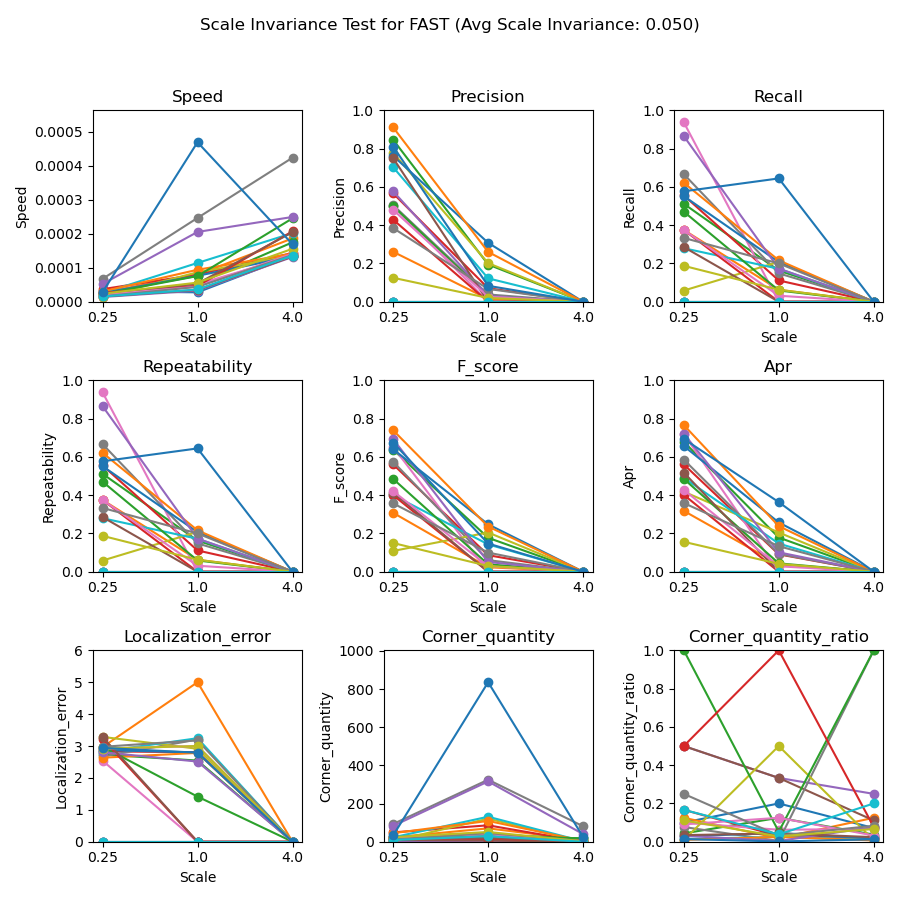
\includegraphics[width=\linewidth]{../results/scale_invariance_plots/FAST_scale_invariance.png}
    \caption{Scale invariance results for FAST, showing metrics across scales [0.25, 1.0, 4.0] for each image, with an average scale invariance score.}
    \label{fig:scale_invariance_fast}
    \end{minipage}
    }
\end{figure}


\onecolumn
\begin{table}
    \centering
    \fbox{
        \begin{minipage}{\textwidth}
    \small
    \caption{Comparison of Corner Detection Algorithms}
    \label{tab:comparison_table}
    \begin{tabular}{lcccccccc}
    \toprule
    \textbf{Algorithm} & \textbf{Precision} & \textbf{Recall} & \textbf{Repeatability} & \textbf{Speed (s)} & \textbf{F Score} & \textbf{APR} & \textbf{Localization Error} & \textbf{Corner Quantity Ratio} \\
    \midrule
    Harris & 0.006 & 0.172 & 0.172 & 0.0004 & 0.011 & 0.089 & 1.698 & 0.001 \\
    Shi-Tomasi & 0.082 & 0.032 & 0.032 & 0.0003 & 0.045 & 0.057 & 1.976 & 0.099 \\
    FAST & 0.070 & 0.117 & 0.117 & 0.0001 & 0.075 & 0.093 & 1.961 & 0.144 \\
    ORB & 0.027 & 0.316 & 0.316 & 0.0008 & 0.044 & 0.171 & 2.382 & 0.019 \\
    SIFT & 0.040 & 0.032 & 0.032 & 0.0061 & 0.028 & 0.036 & 1.423 & 0.104 \\
    BRISK & 0.025 & 0.439 & 0.439 & 0.0314 & 0.044 & 0.232 & 2.252 & 0.003 \\
    AGAST & 0.069 & 0.101 & 0.101 & 0.0002 & 0.049 & 0.085 & 1.843 & 0.136 \\
    KAZE & 0.062 & 0.056 & 0.056 & 0.0046 & 0.054 & 0.059 & 1.962 & 0.160 \\
    AKAZE & 0.072 & 0.066 & 0.066 & 0.0022 & 0.066 & 0.069 & 1.943 & 0.138 \\
    \bottomrule
    \end{tabular}
    \end{minipage}
    }
\end{table}

\twocolumn

%%%%%%%%%%%%%%%%%%%%%%%%%%%%%%%%%%%%%%%%%%%%%%%%%%%%%%%%%%%%%%%%%%%%%%%%%%%%%%%%%%%%%%%%%%%%

\section{Analysis}
\label{section:analysis}

The benchmarking results highlight important trade-offs between detection accuracy, computational speed, and robustness among the evaluated algorithms. FAST and AGAST demonstrated the best computational efficiency, achieving mean execution times below 0.0002 seconds per image (Table~\ref{tab:comparison_table}). These detectors are highly suitable for real-time applications but sacrificed some detection accuracy. FAST achieved relatively low precision (0.025) and recall (0.102), while AGAST achieved slightly better precision (0.059) and recall (0.101). SIFT and KAZE, while significantly slower (mean execution times above 0.003 seconds), exhibited stronger detection quality. KAZE achieved the lowest mean localization error (1.331 pixels), indicating the most accurate corner positioning relative to ground truth. SIFT demonstrated better scale robustness compared to most detectors, achieving a scale invariance score of 0.081 (Table~\ref{tab:scale_invariance_scores}). BRISK achieved the highest recall (0.439), detecting a large number of corners. However, it suffered from extremely low precision (0.025), suggesting a high rate of false positive detections. This is corroborated by BRISK’s corner quantity ratio, which was high (0.160), indicating significant over-detection relative to the number of ground truth corners. ORB, while designed for efficiency, performed moderately across all metrics, achieving good speed (0.0003 seconds), modest precision (0.074), and moderate repeatability (0.338). However, its scale invariance score (0.045) was among the lowest, indicating poor robustness to large changes in image scale. In terms of repeatability, KAZE and SIFT performed well (0.381 and 0.368, respectively), confirming their ability to detect consistent corners across different images and scales. Harris and Shi-Tomasi, classical methods, exhibited moderate repeatability but struggled in precision and recall, especially Harris with a precision of only 0.002. Scale invariance results further emphasized the strengths and weaknesses of different detectors. BRISK achieved the highest scale invariance score (0.443), followed by AKAZE (0.105) and Shi-Tomasi (0.118), indicating their robustness to significant scale changes. In contrast, FAST and ORB exhibited poor scale invariance (scores of 0.050 and 0.045, respectively), consistent with their simple, fast design priorities. Finally, considering the aggregate performance scores (Table~\ref{tab:comparison_table}), AGAST emerged as the overall best-performing detector in this study, achieving a balanced trade-off between detection quality and computational efficiency.\\

Overall, the results emphasize that no single detector is universally optimal. Instead, algorithm choice should be driven by application-specific requirements, such as prioritizing speed (e.g., FAST, AGAST) versus prioritizing accuracy and robustness (e.g., KAZE, SIFT).\\


%%%%%%%%%%%%%%%%%%%%%%%%%%%%%%%%%%%%%%%%%%%%%%%%%%%%%%%%%%%%%%%%%%%%%%%%%%%%%%%%%%%%%%%%%%%%

\section{Conclusion}
\label{section:conclusion}

This project implemented a benchmarking framework for evaluating nine OpenCV corner detection algorithms under varying parameter configurations and image scales. Metrics including precision, recall, repeatability, execution time, and scale robustness were systematically analyzed across a diverse urban dataset.

Among the evaluated methods, AGAST provided the best balance between speed and accuracy for practical use cases, while SIFT and KAZE excelled in scale robustness at the cost of speed. The results emphasize that no single algorithm is universally optimal; the best choice depends on specific application requirements.

Future work could extend the framework by incorporating more advanced detectors such as SuperPoint or R2D2, evaluating robustness to additional distortions like rotation and illumination changes, and exploring learning-based parameter optimization techniques. Further, testing on larger and more varied datasets would provide deeper insights into algorithm generalization.

%%%%%%%%%%%%%%%%%%%%%%%%%%%%%%%%%%%%%%%%%%%%%%%%%%%%%%%%%%%%%%%%%%%%%%%%%%%%%%%%%%%%%%%%%%%%

\bibliographystyle{IEEEtran}
\bibliography{references}

\begin{thebibliography}{1}

    \bibitem{MDPI_Benchmark} 
    J. Doe et al., "A Benchmark Dataset for Corner Detection," \textit{MDPI}, 2022. [Online]. Available: \url{https://www.mdpi.com/2076-3417/12/23/11984}.

    \bibitem{OpenCV_Doc} 
    OpenCV Documentation, \url{https://docs.opencv.org}. Accessed: 2025.

    \bibitem{Harris_Corner} 
    C. Harris and M. Stephens, "A Combined Corner and Edge Detector," in \textit{Proc. 4th Alvey Vision Conf.}, 1988.

    \bibitem{Shi_Tomasi} 
    J. Shi and C. Tomasi, "Good Features to Track," in \textit{Proc. IEEE Conf. Computer Vision and Pattern Recognition (CVPR)}, 1994.

    \bibitem{FAST} 
    E. Rosten and T. Drummond, "Fusing points and lines for high performance tracking," in \textit{Proc. IEEE Int. Conf. Computer Vision}, 2005.

    \bibitem{ORB} 
    E. Rublee, V. Rabaud, K. Konolige, and G. Bradski, "ORB: An Efficient Alternative to SIFT or SURF," in \textit{Proc. IEEE Int. Conf. Computer Vision}, 2011.

    \bibitem{SIFT} 
    D. G. Lowe, "Distinctive image features from scale-invariant keypoints," \textit{Int. J. Computer Vision}, 2004.

    \bibitem{BRISK} 
    L. Leutenegger, M. Chli, and R. Siegwart, "BRISK: Binary Robust Invariant Scalable Keypoints," in \textit{Proc. IEEE Int. Conf. Computer Vision}, 2011.

    \bibitem{AGAST} 
    M. Mair, A. A. Bartoli, and L. van Gool, "AGAST: Adaptive and Generic Accelerated Segment Test for Corner Detection," \textit{Pattern Recognition Letters}, 2011.

    \bibitem{KAZE} 
    P. Alcantarilla, A. Bartoli, and L. Van Gool, "KAZE Features," in \textit{Proc. European Conf. Computer Vision}, 2012.

    \bibitem{Urban_Corner_Dataset}
    Y. Zhang, "Urban Corner Datasets," GitHub, 2023. [Online]. Available: \url{https://github.com/yangzhangcv/Urban_Corner-datasets}.

\end{thebibliography}

%%%%%%%%%%%%%%%%%%%%%%%%%%%%%%%%%%%%%%%%%%%%%%%%%%%%%%%%%%%%%%%%%%%%%%%%%%%%%%%%%%%%%%%%%%%%

% \onecolumn
% \twocolumn

\appendices
\section{Optimization Results: Images and Plots}
\label{app:optimization_results}
\begin{figure}[h]
    \centering
    \fbox{
        \begin{minipage}{0.47\textwidth}
    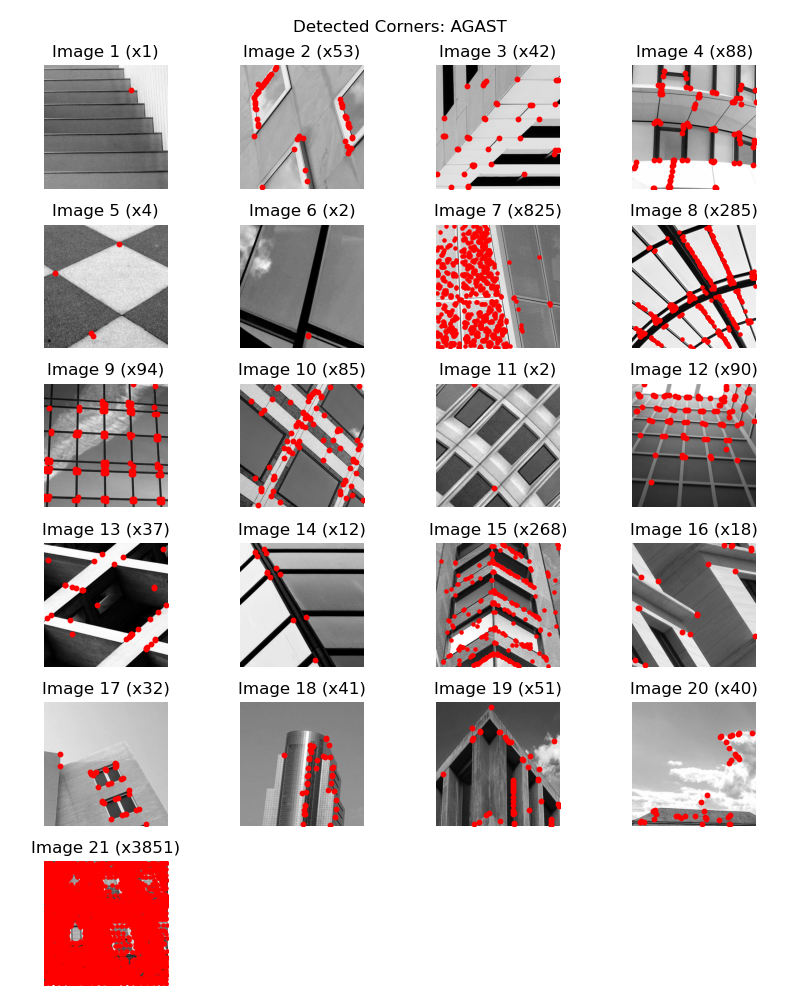
\includegraphics[width=\linewidth]{../results/sample_detections/AGAST_all_detections.png}
    \caption{Sample detection for AGAST on a randomly selected image, with ground truth corners (green circles) and detected corners (red circles).}
    \label{fig:agast_samp}
    \end{minipage}
    }
\end{figure}

\begin{figure}[h]
    \centering
    \fbox{
        \begin{minipage}{0.47\textwidth}
    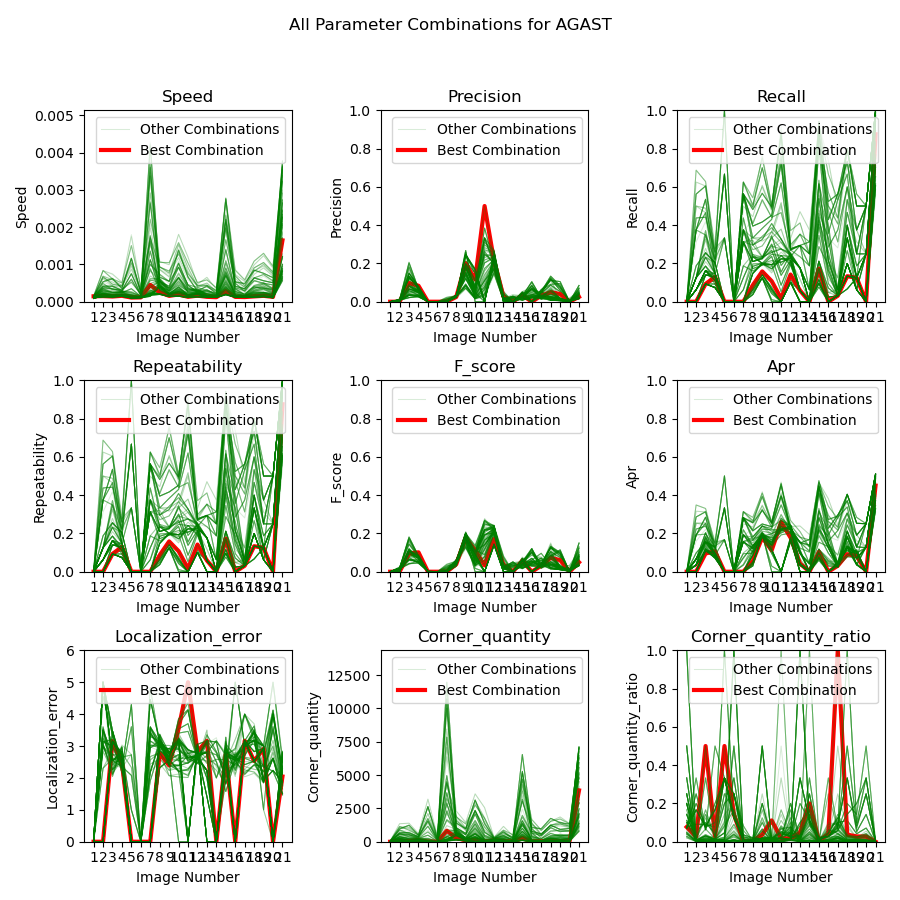
\includegraphics[width=\linewidth]{../results/all_combinations_plots/AGAST_all_combinations.png}
    \caption{Best parameter combination metrics for the AGAST algorithm across individual images, showing precision, recall, repeatability, F-score, APR, localization error, corner quantity, corner quantity ratio, and speed.}
    \label{fig:agast_combs}
    \end{minipage}
    }
\end{figure}

\begin{figure}[h]
    \centering
    \fbox{
        \begin{minipage}{0.47\textwidth}
    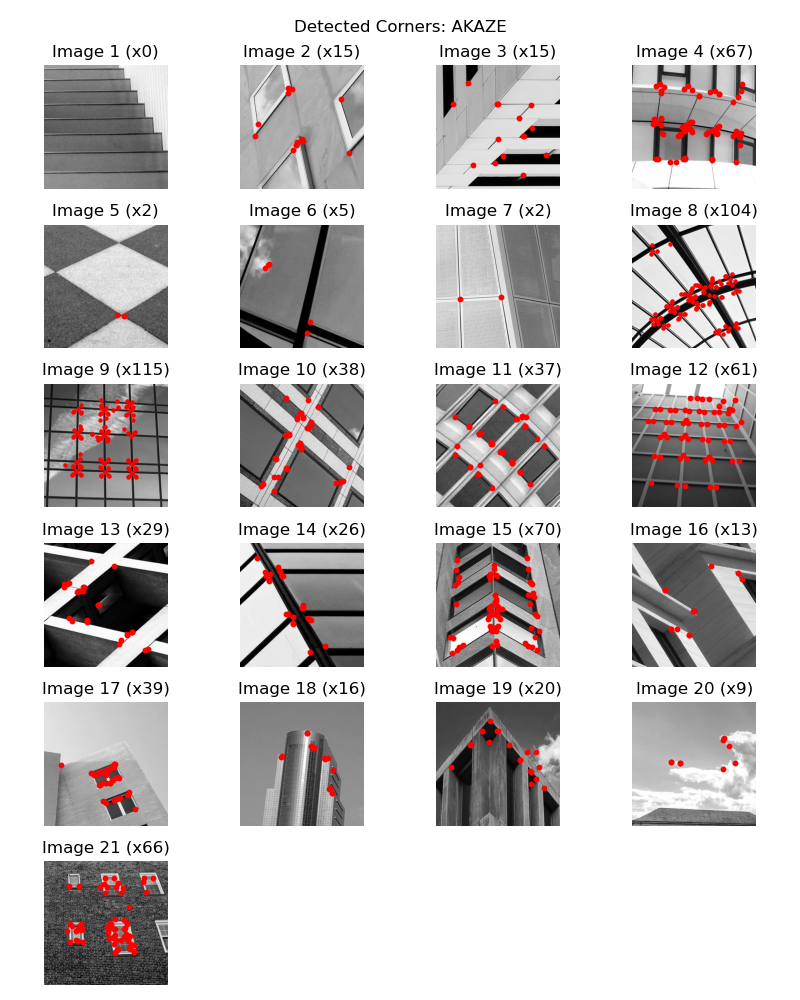
\includegraphics[width=\linewidth]{../results/sample_detections/AKAZE_all_detections.png}
    \caption{Sample detection for AKAZE on a randomly selected image, with ground truth corners (green circles) and detected corners (red circles).}
    \label{fig:akaze_samp}
    \end{minipage}
    }
\end{figure}

\begin{figure}[h]
    \centering
    \fbox{
        \begin{minipage}{0.47\textwidth}
    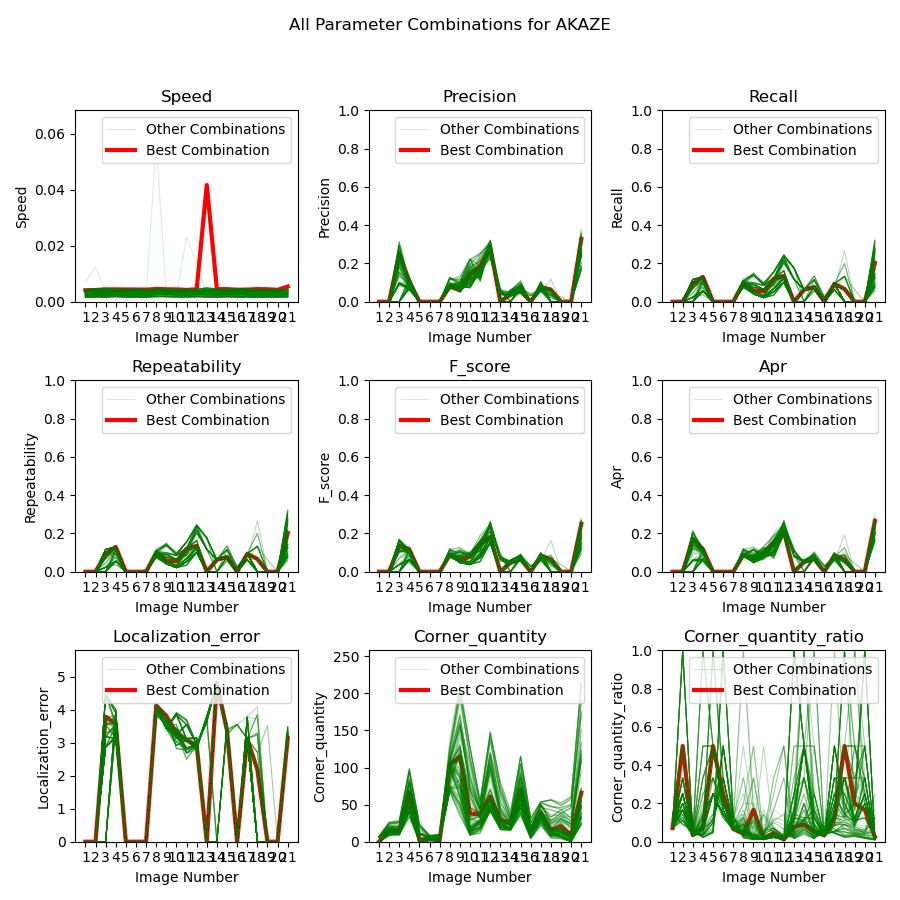
\includegraphics[width=\linewidth]{../results/all_combinations_plots/AKAZE_all_combinations.png}
    \caption{Best parameter combination metrics for the AKAZE algorithm across individual images, showing precision, recall, repeatability, F-score, APR, localization error, corner quantity, corner quantity ratio, and speed.}
    \label{fig:akaze_combs}
    \end{minipage}
    }
\end{figure}

\begin{figure}[h]
    \centering
    \fbox{
        \begin{minipage}{0.47\textwidth}
    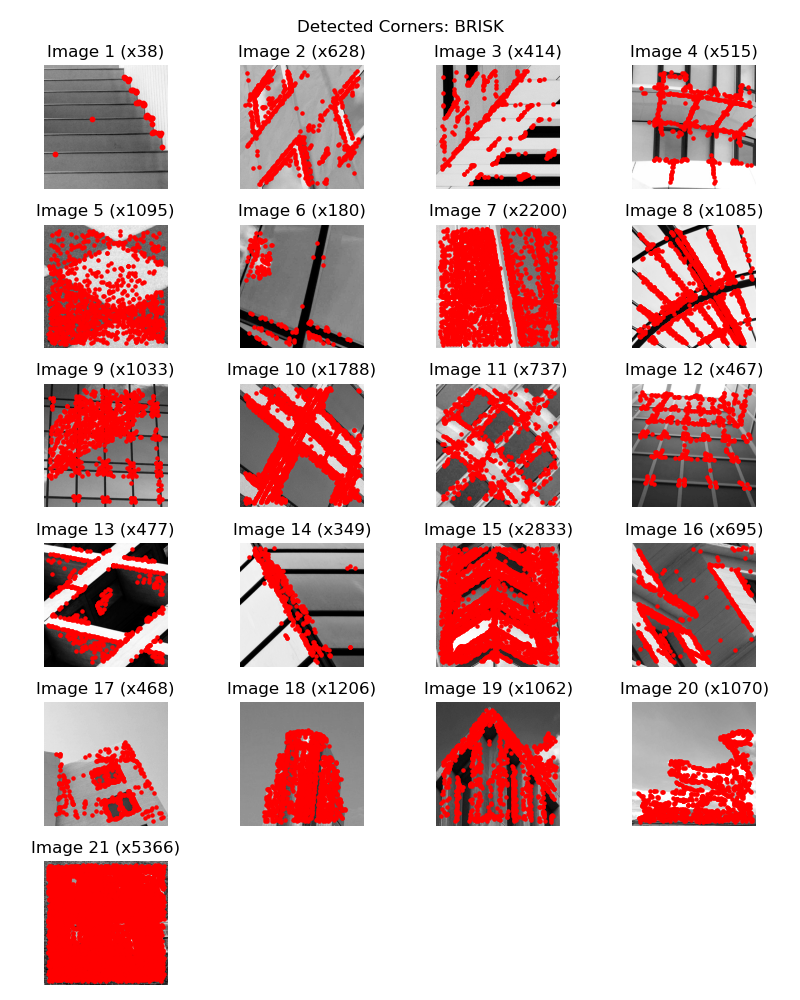
\includegraphics[width=\linewidth]{../results/sample_detections/BRISK_all_detections.png}
    \caption{Sample detection for BRISK on a randomly selected image, with ground truth corners (green circles) and detected corners (red circles).}
    \label{fig:brisk_samp}
    \end{minipage}
    }
\end{figure}

\begin{figure}[h]
    \centering
    \fbox{
        \begin{minipage}{0.47\textwidth}
    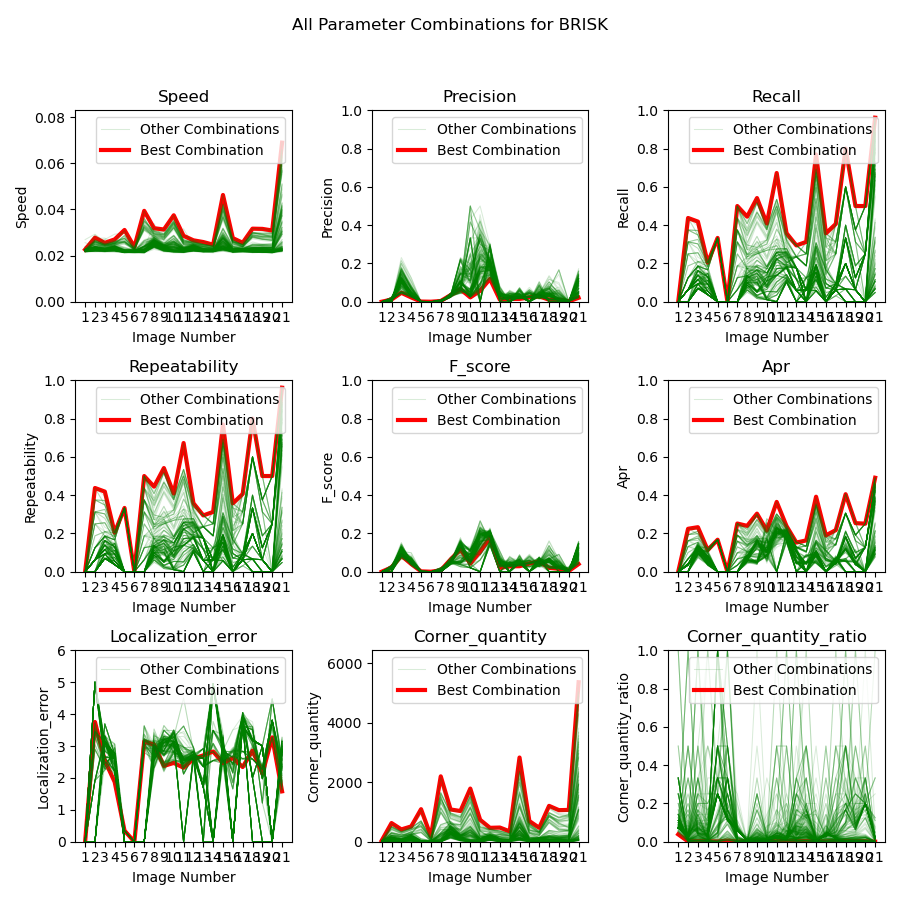
\includegraphics[width=\linewidth]{../results/all_combinations_plots/BRISK_all_combinations.png}
    \caption{Best parameter combination metrics for the BRISK algorithm across individual images, showing precision, recall, repeatability, F-score, APR, localization error, corner quantity, corner quantity ratio, and speed.}
    \label{fig:brisk_combs}
    \end{minipage}
    }
\end{figure}

\begin{figure}[h]
    \centering
    \fbox{
        \begin{minipage}{0.47\textwidth}
    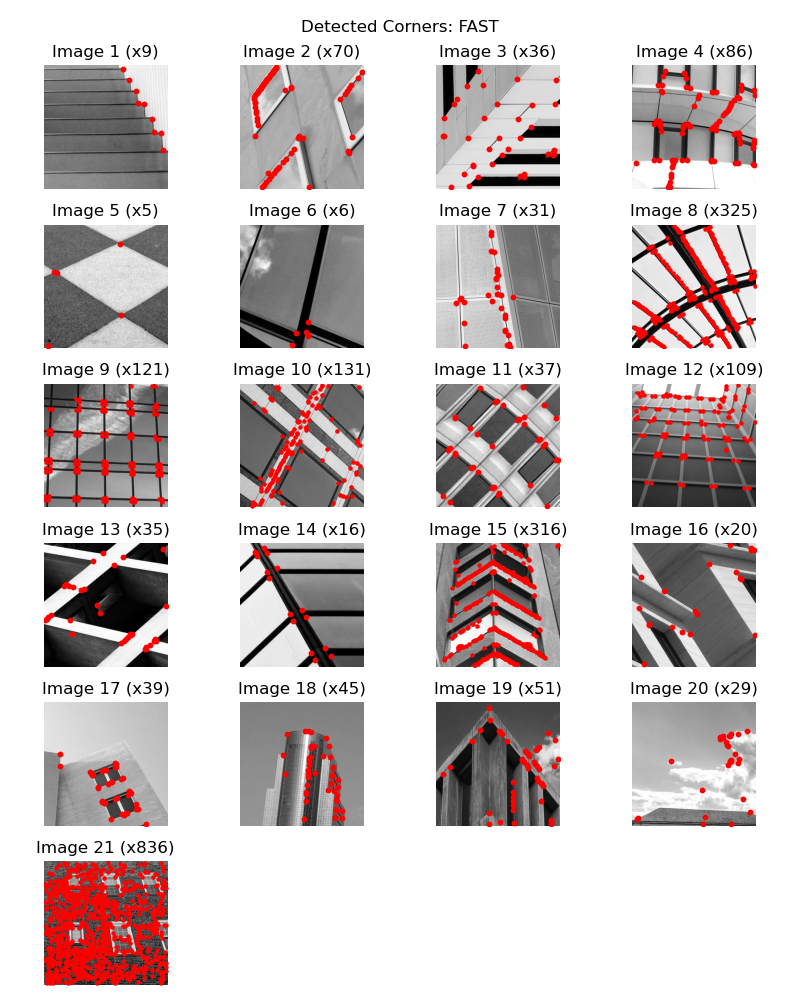
\includegraphics[width=\linewidth]{../results/sample_detections/FAST_all_detections.png}
    \caption{Sample detection for FAST on a randomly selected image, with ground truth corners (green circles) and detected corners (red circles).}
    \label{fig:fast_samp}
    \end{minipage}
    }
\end{figure}


\begin{figure}[h]
    \centering
    \fbox{
        \begin{minipage}{0.47\textwidth}
    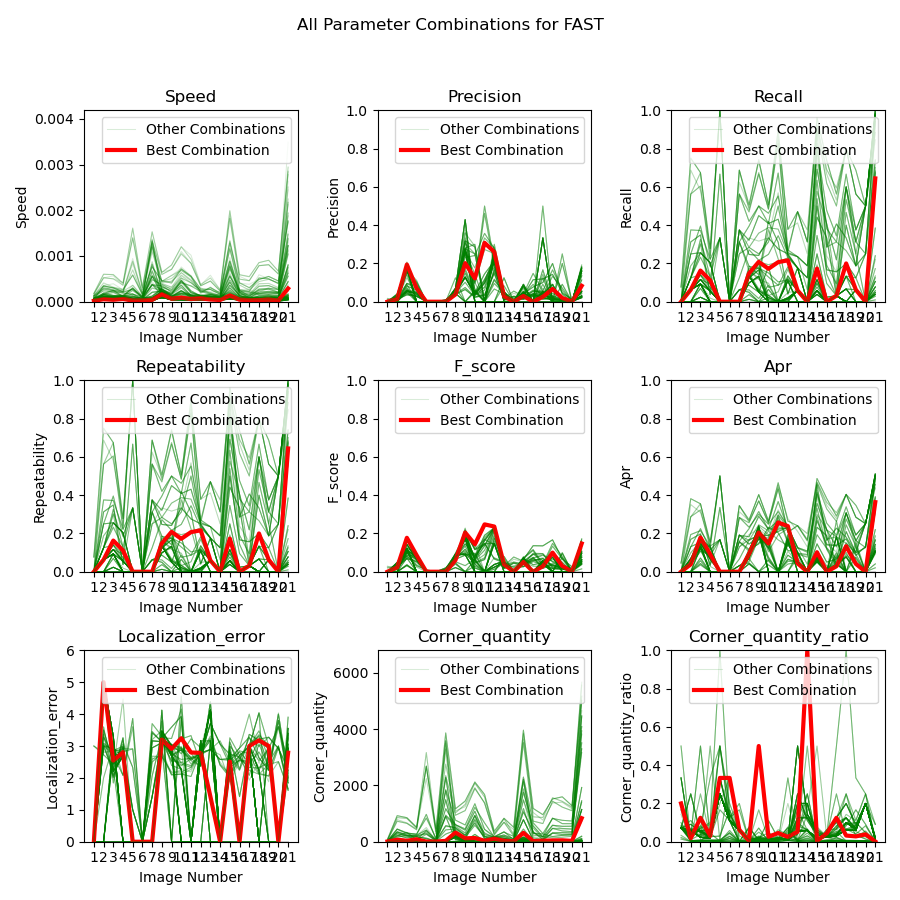
\includegraphics[width=\linewidth]{../results/all_combinations_plots/FAST_all_combinations.png}
    \caption{Best parameter combination metrics for the FAST algorithm across individual images, showing precision, recall, repeatability, F-score, APR, localization error, corner quantity, corner quantity ratio, and speed.}
    \label{fig:fast_combs}
    \end{minipage}
    }
\end{figure}

\begin{figure}[h]
    \centering
    \fbox{
        \begin{minipage}{0.47\textwidth}
    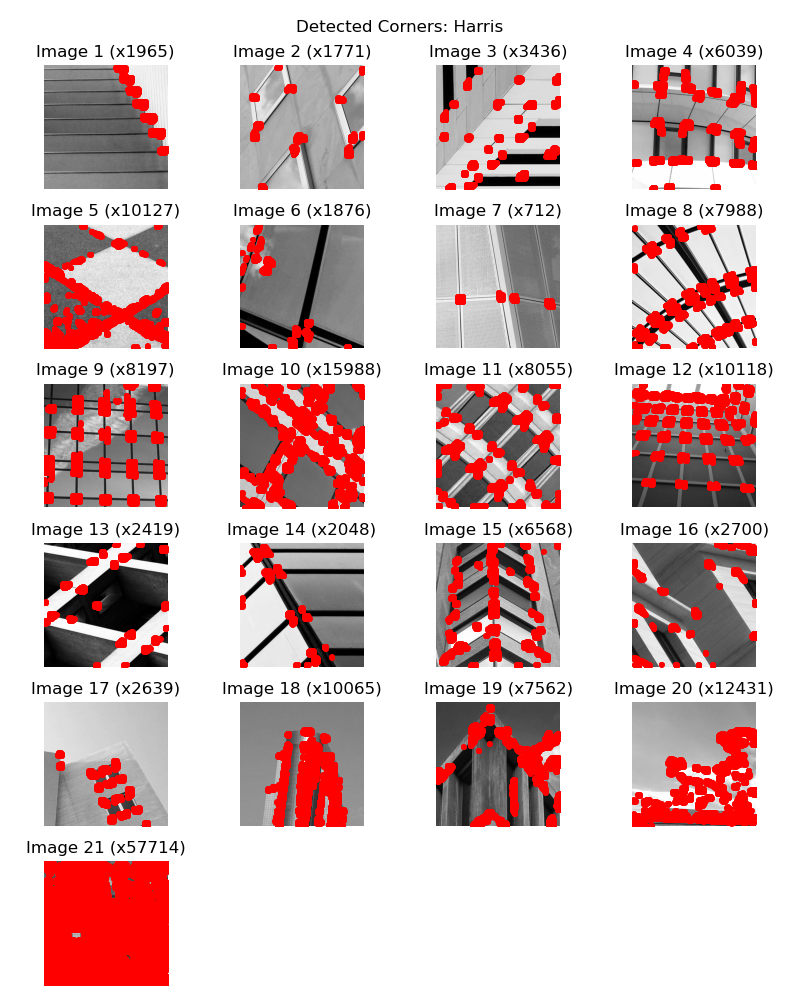
\includegraphics[width=\linewidth]{../results/sample_detections/Harris_all_detections.png}
    \caption{Sample detection for Harris on a randomly selected image, with ground truth corners (green circles) and detected corners (red circles).}
    \label{fig:harris_samp}
    \end{minipage}
    }
\end{figure}

\begin{figure}[h]
    \centering
    \fbox{
        \begin{minipage}{0.47\textwidth}
    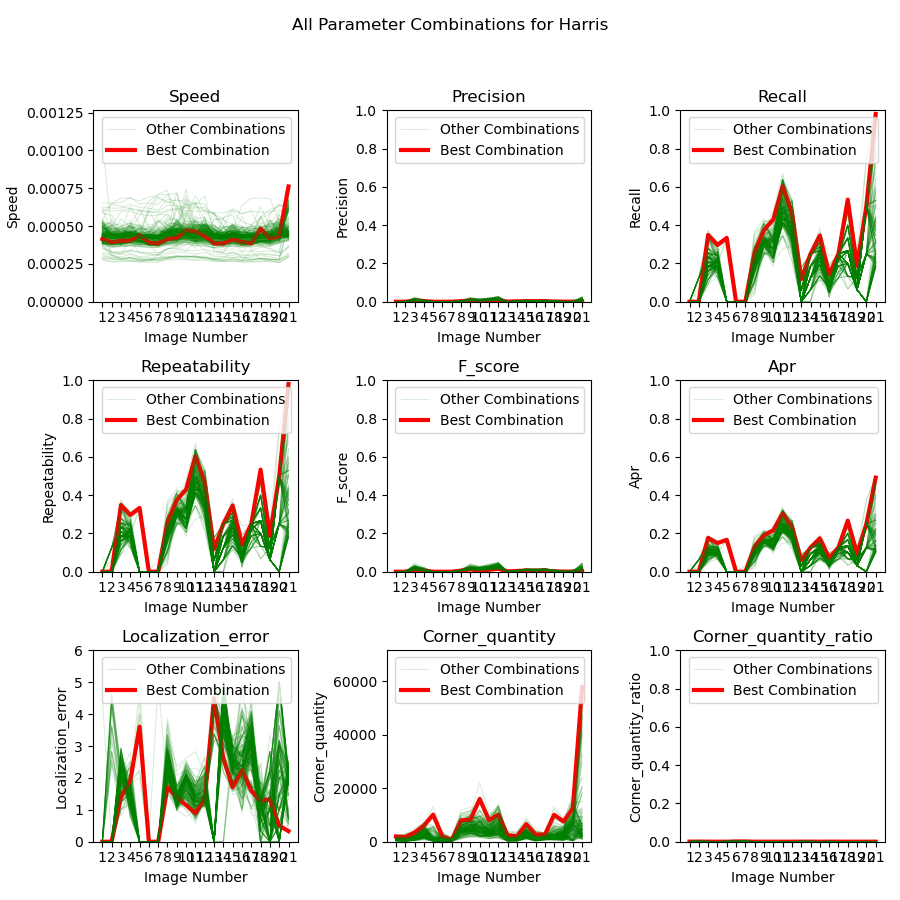
\includegraphics[width=\linewidth]{../results/all_combinations_plots/Harris_all_combinations.png}
    \caption{Best parameter combination metrics for the Harris algorithm across individual images, showing precision, recall, repeatability, F-score, APR, localization error, corner quantity, corner quantity ratio, and speed.}
    \label{fig:harris_combs}
    \end{minipage}
    }
\end{figure}

\begin{figure}[h]
    \centering
    \fbox{
        \begin{minipage}{0.47\textwidth}
    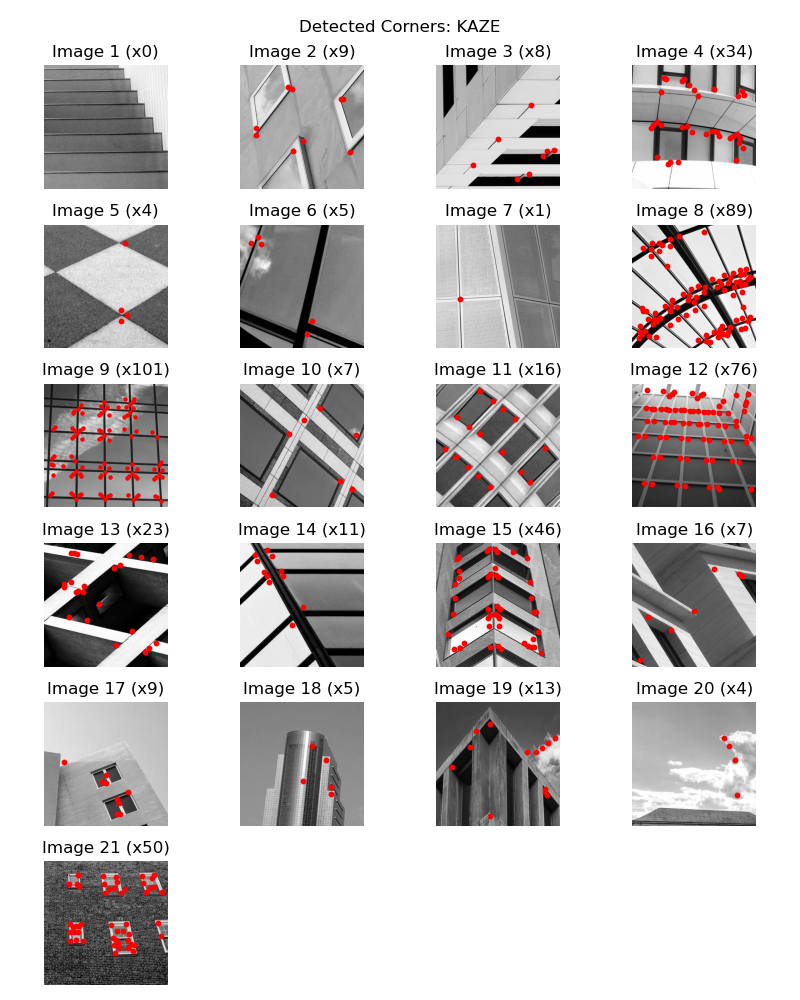
\includegraphics[width=\linewidth]{../results/sample_detections/KAZE_all_detections.png}
    \caption{Sample detection for KAZE on a randomly selected image, with ground truth corners (green circles) and detected corners (red circles).}
    \label{fig:kaze_samp}
    \end{minipage}
    }
\end{figure}

\begin{figure}[h]
    \centering
    \fbox{
        \begin{minipage}{0.47\textwidth}
    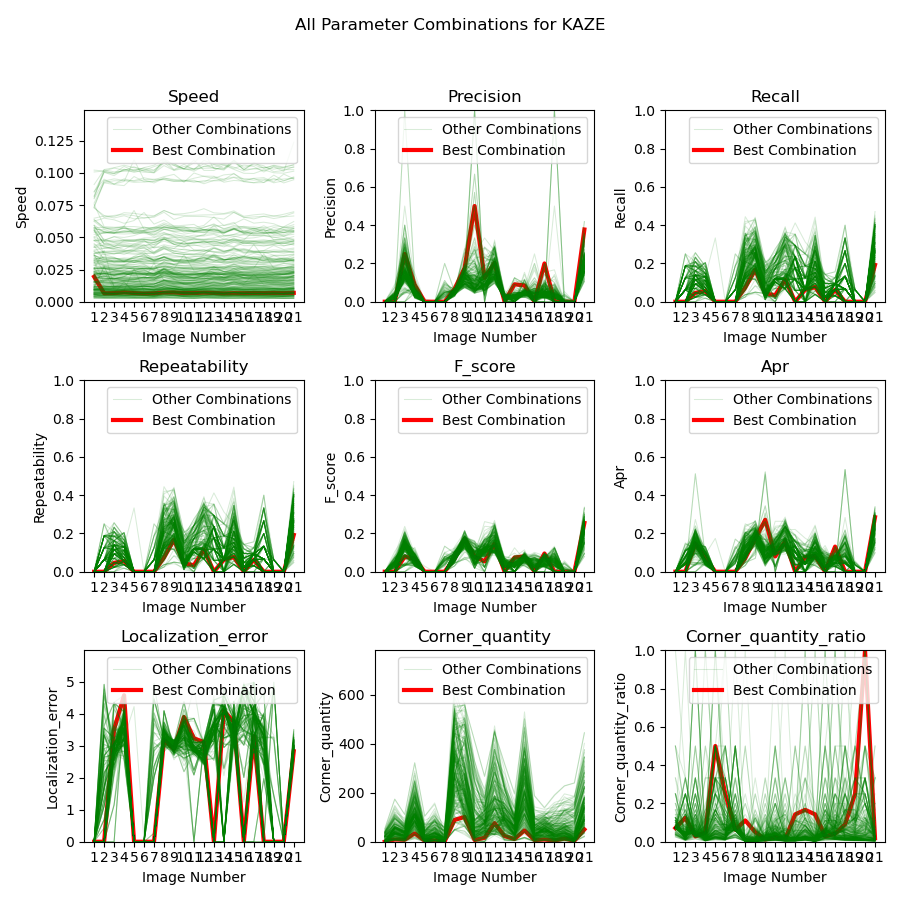
\includegraphics[width=\linewidth]{../results/all_combinations_plots/KAZE_all_combinations.png}
    \caption{Best parameter combination metrics for the KAZE algorithm across individual images, showing precision, recall, repeatability, F-score, APR, localization error, corner quantity, corner quantity ratio, and speed.}
    \label{fig:kaze_combs}
    \end{minipage}
    }
\end{figure}


\begin{figure}[h]
    \centering
    \fbox{
        \begin{minipage}{0.47\textwidth}
    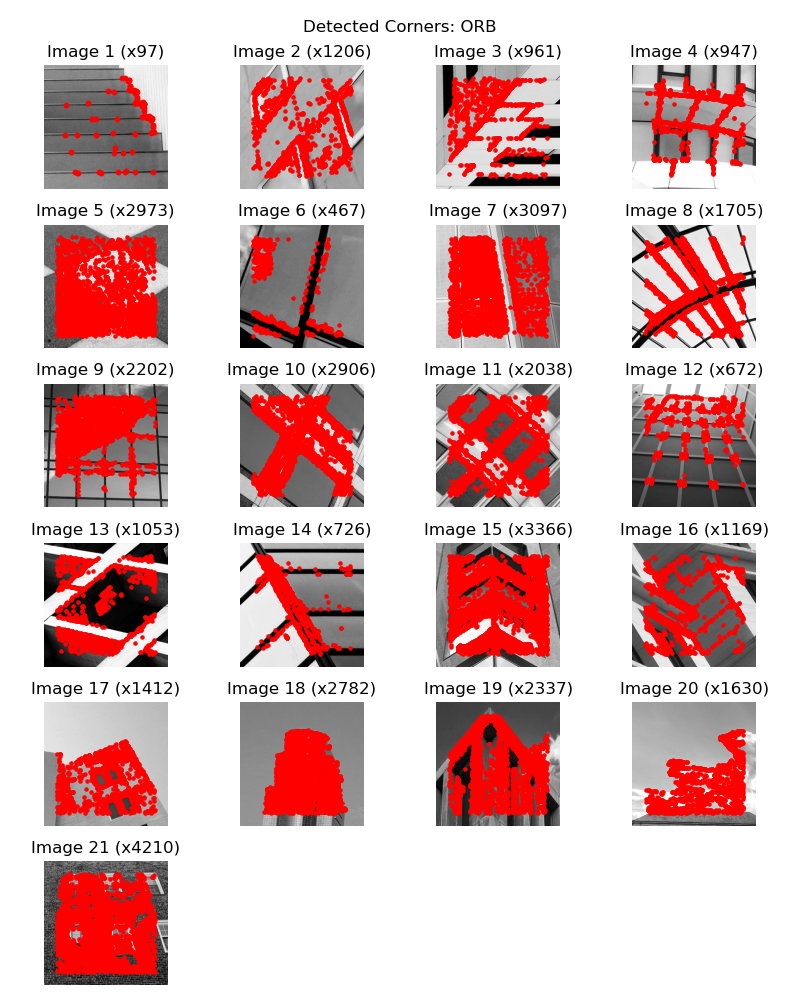
\includegraphics[width=\linewidth]{../results/sample_detections/ORB_all_detections.png}
    \caption{Sample detection for ORB on a randomly selected image, with ground truth corners (green circles) and detected corners (red circles).}
    \label{fig:orb_samp}
    \end{minipage}
    }
\end{figure}

\begin{figure}[h]
    \centering
    \fbox{
        \begin{minipage}{0.47\textwidth}
    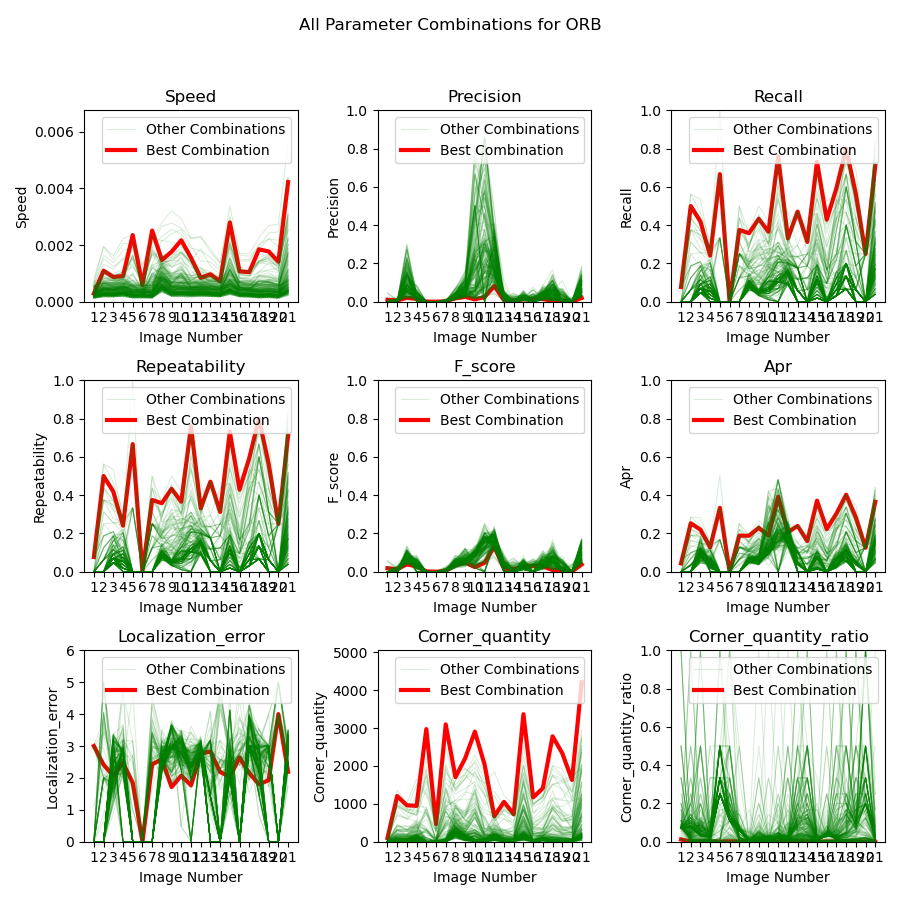
\includegraphics[width=\linewidth]{../results/all_combinations_plots/ORB_all_combinations.png}
    \caption{Best parameter combination metrics for the ORB algorithm across individual images, showing precision, recall, repeatability, F-score, APR, localization error, corner quantity, corner quantity ratio, and speed.}
    \label{fig:orb_combs}
    \end{minipage}
    }
\end{figure}

\begin{figure}[h]
    \centering
    \fbox{
        \begin{minipage}{0.47\textwidth}
    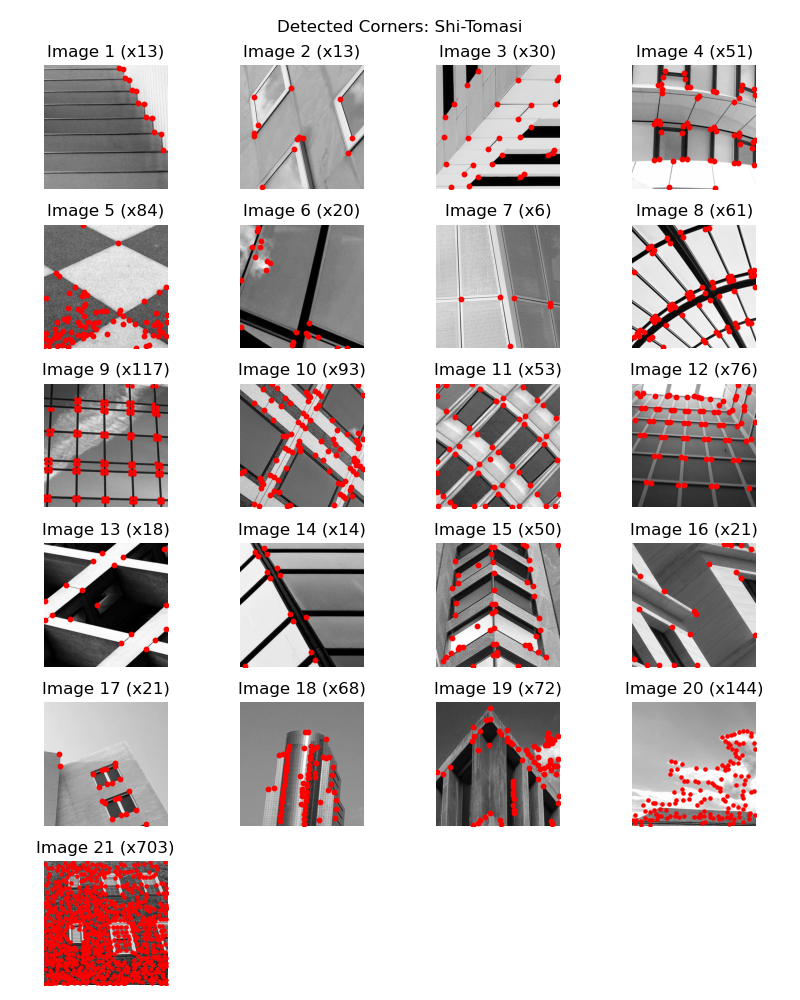
\includegraphics[width=\linewidth]{../results/sample_detections/Shi-Tomasi_all_detections.png}
    \caption{Sample detection for Shi-Tomasi on a randomly selected image, with ground truth corners (green circles) and detected corners (red circles).}
    \label{fig:shi_samp}
    \end{minipage}
    }
\end{figure}

\begin{figure}[h]
    \centering
    \fbox{
        \begin{minipage}{0.47\textwidth}
    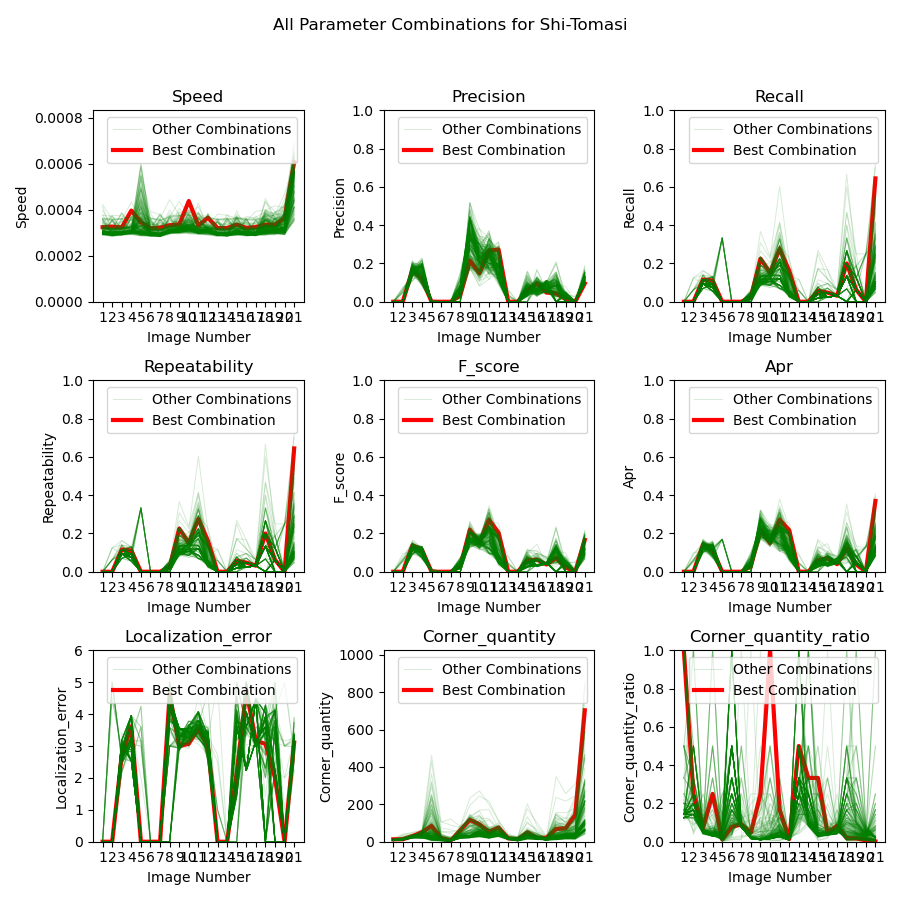
\includegraphics[width=\linewidth]{../results/all_combinations_plots/Shi-Tomasi_all_combinations.png}
    \caption{Best parameter combination metrics for the Shi-Tomasi algorithm across individual images, showing precision, recall, repeatability, F-score, APR, localization error, corner quantity, corner quantity ratio, and speed.}
    \label{fig:shi_combs}
    \end{minipage}
    }
\end{figure}


\begin{figure}[h]
    \centering
    \fbox{
        \begin{minipage}{0.47\textwidth}
    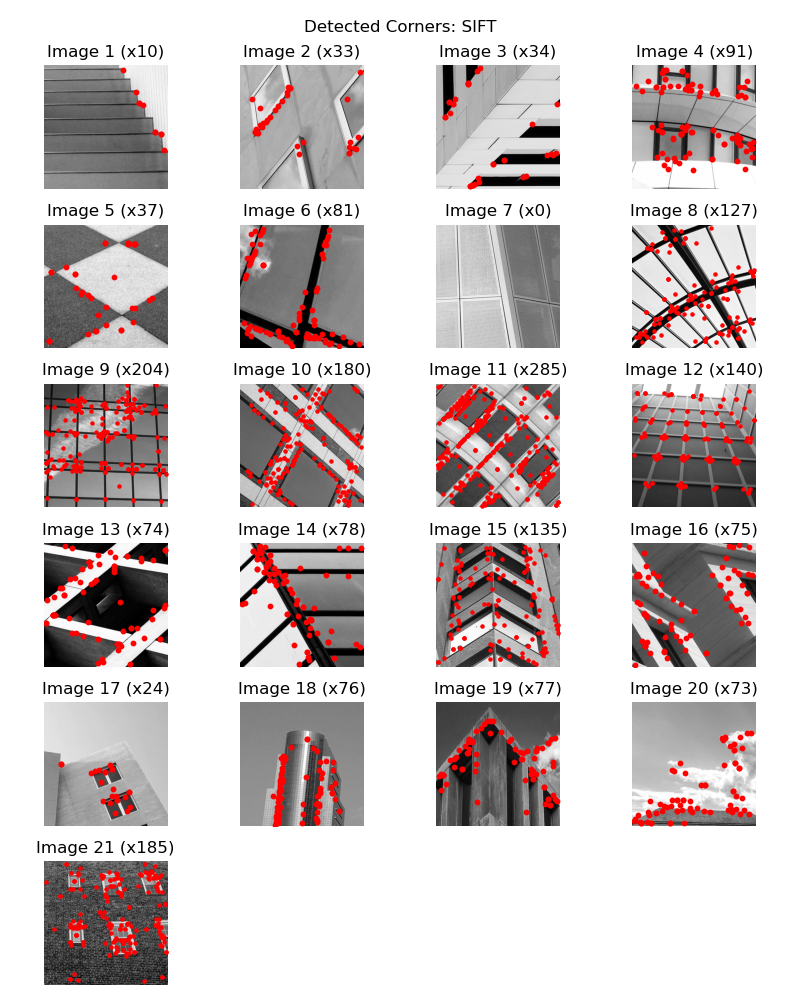
\includegraphics[width=\linewidth]{../results/sample_detections/SIFT_all_detections.png}
    \caption{Sample detection for SIFT on a randomly selected image, with ground truth corners (green circles) and detected corners (red circles).}
    \label{fig:sift_samp}
    \end{minipage}
    }
\end{figure}

\begin{figure}[h]
    \centering
    \fbox{
        \begin{minipage}{0.47\textwidth}
    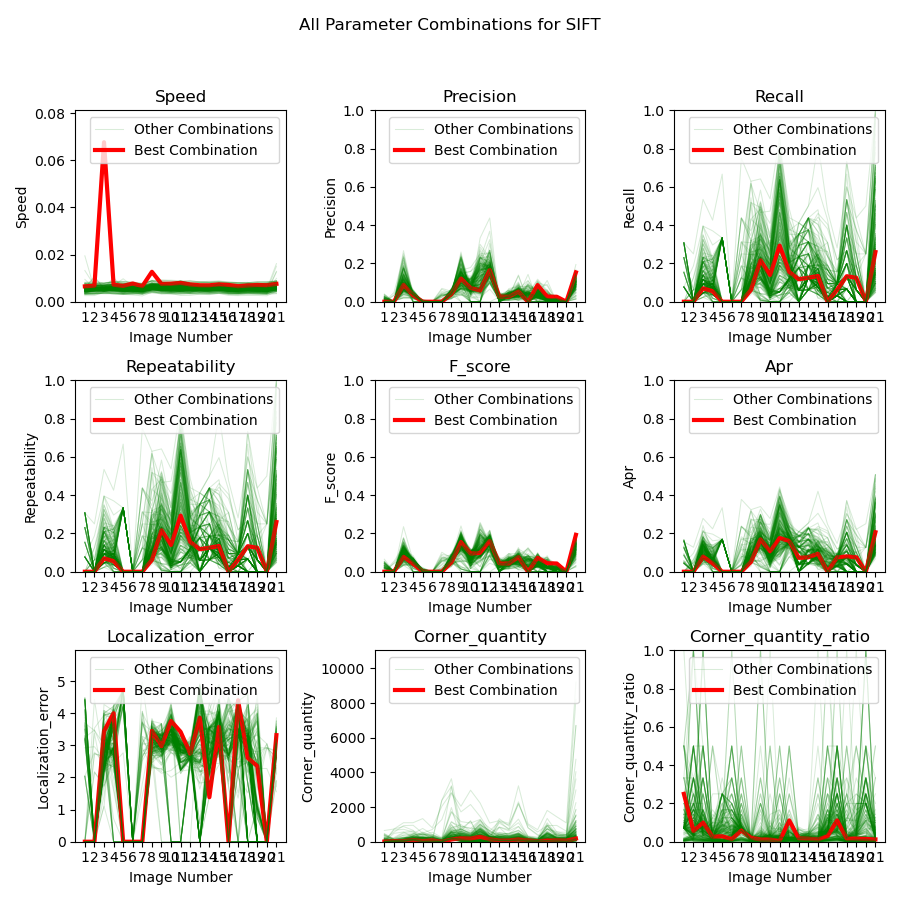
\includegraphics[width=\linewidth]{../results/all_combinations_plots/SIFT_all_combinations.png}
    \caption{Best parameter combination metrics for the SIFT algorithm across individual images, showing precision, recall, repeatability, F-score, APR, localization error, corner quantity, corner quantity ratio, and speed.}
    \label{fig:sift_combs}
    \end{minipage}
    }
\end{figure}


%%%%%%%%%%%%%%%%%%%%%%%%%%%%%%%%%%%%%%%%%%%%%%%%%%%%%%%%%%%%%%%%%%%%%%%%%%%%%%%%%%%%%%%%%%%%


%%%%%%%%%%%%%%%%%%%%%%%%%%%%%%%%%%%%%%%%%%%%%%%%%%%%%%%%%%%%%%%%%%%%%%%%%%%%%%%%%%%%%%%%%%%%

\section{Scale Invariance Results: Images and Plots}

\label{app:scale_invariance_results}


\begin{figure}[h]
    \centering
    \fbox{
        \begin{minipage}{0.47\textwidth}
    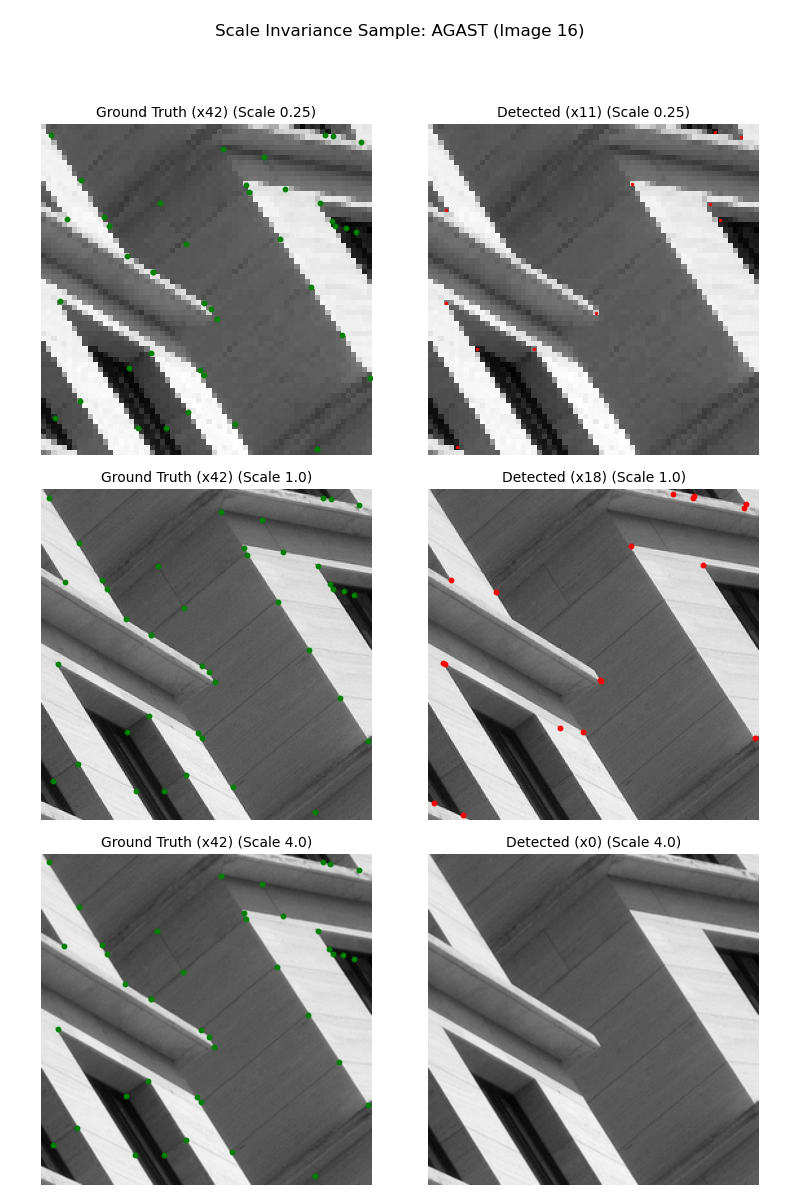
\includegraphics[width=\linewidth]{../results/scale_invariance_samples/AGAST_scale_invariance_sample.png}
    \caption{Scale invariance sample for AGAST on a randomly selected image, showing ground truth (green circles) and detected corners (red circles) at scales [0.25, 1.0, 4.0].}
    \end{minipage}
    }
\end{figure}

\begin{figure}[h]
    \centering
    \fbox{
        \begin{minipage}{0.47\textwidth}
    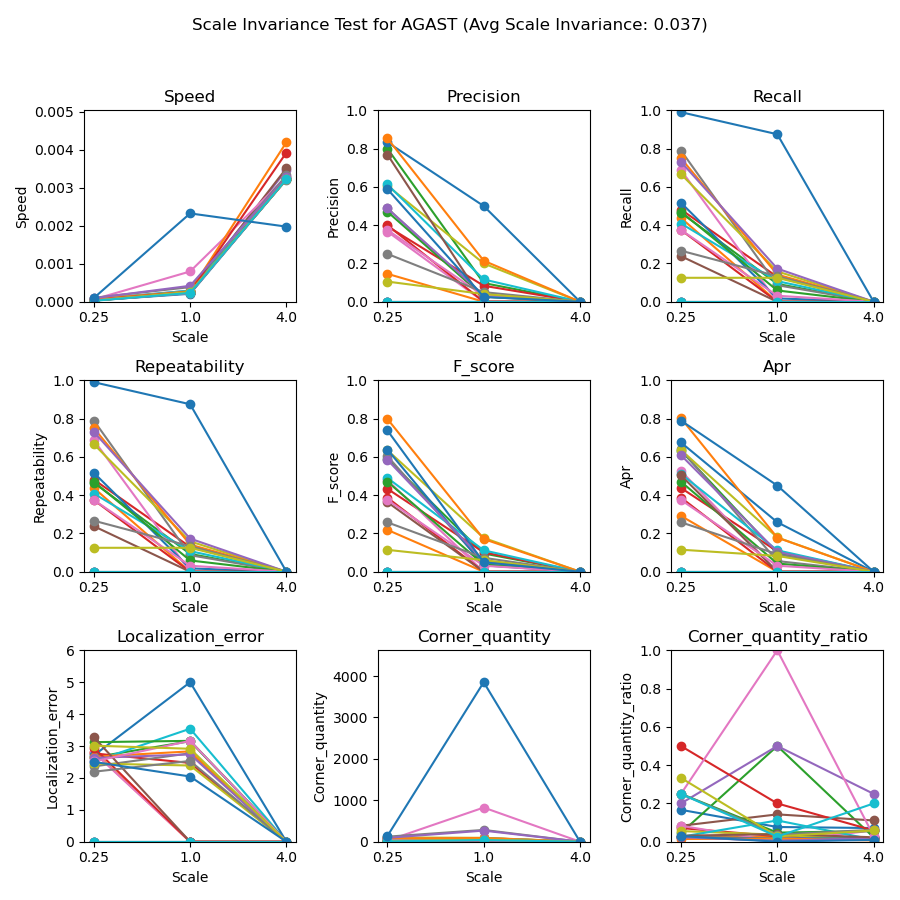
\includegraphics[width=\linewidth]{../results/scale_invariance_plots/AGAST_scale_invariance.png}
    \caption{Scale invariance results for AGAST, showing metrics across scales [0.25, 1.0, 4.0] for each image, with an average scale invariance score.}
    \end{minipage}
    }
\end{figure}

\begin{figure}[h]
    \centering
    \fbox{
        \begin{minipage}{0.47\textwidth}
    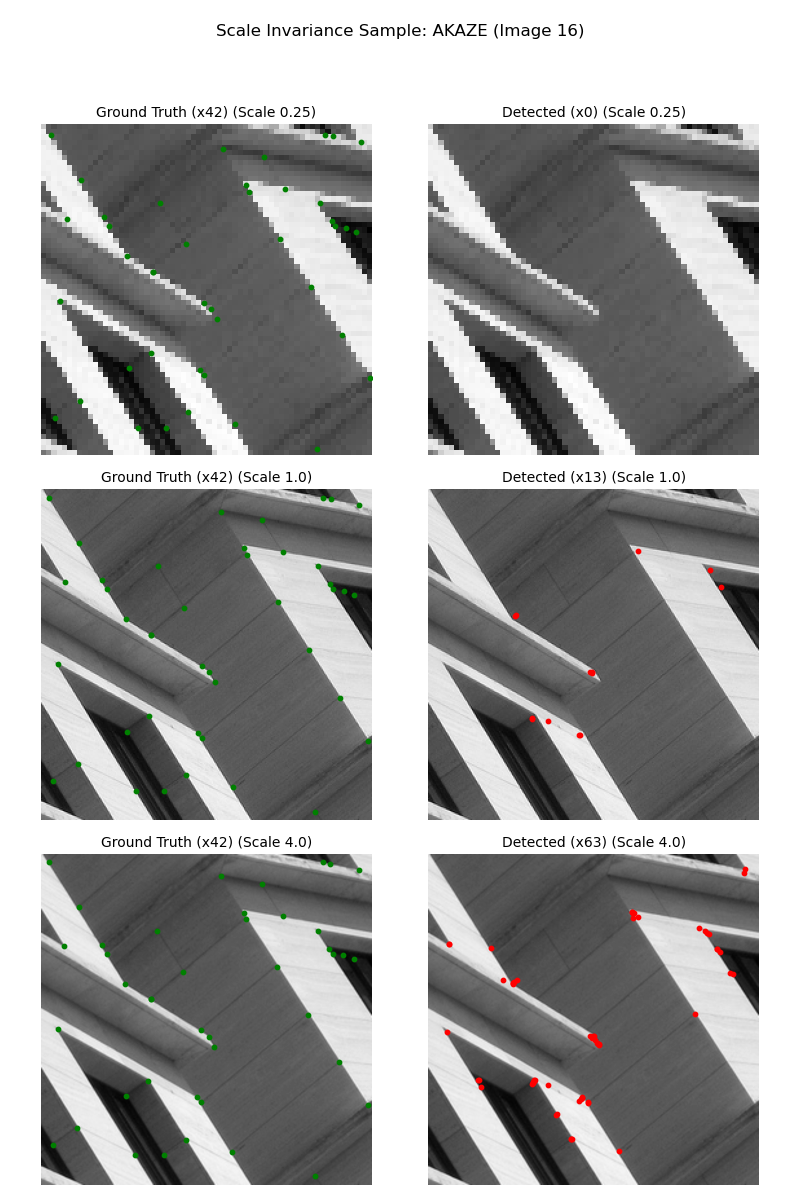
\includegraphics[width=\linewidth]{../results/scale_invariance_samples/AKAZE_scale_invariance_sample.png}
    \caption{Scale invariance sample for AKAZE on a randomly selected image, showing ground truth (green circles) and detected corners (red circles) at scales [0.25, 1.0, 4.0].}
    \end{minipage}
    }
\end{figure}

\begin{figure}[h]
    \centering
    \fbox{
        \begin{minipage}{0.47\textwidth}
    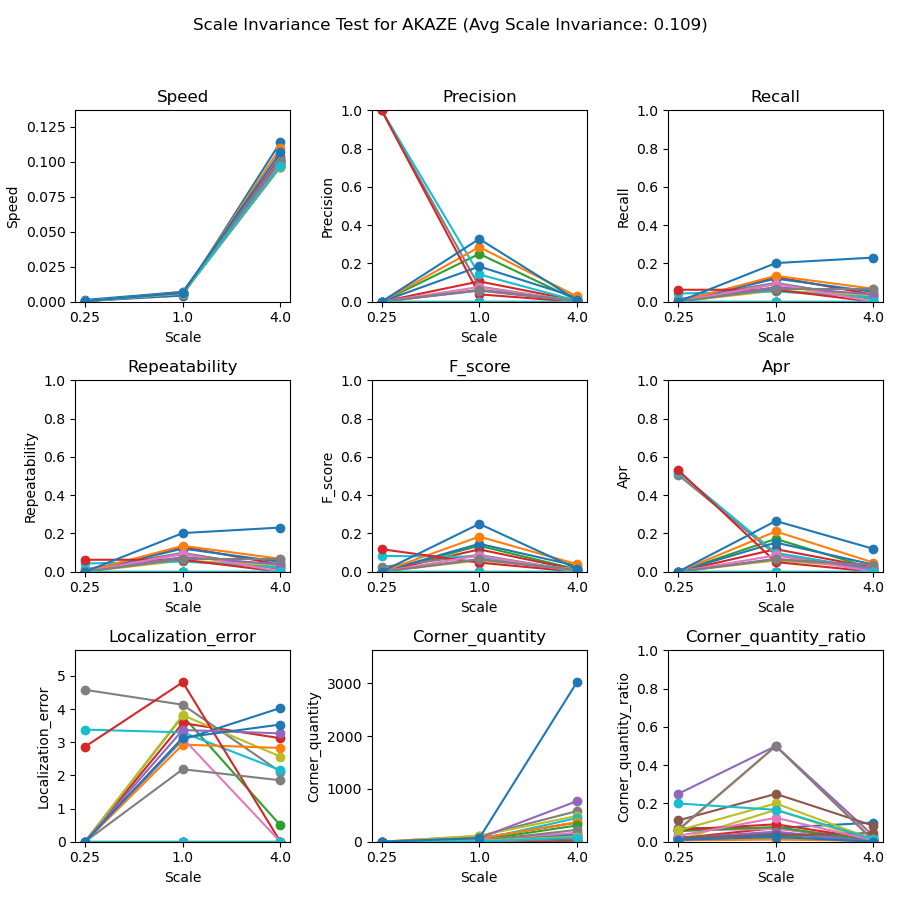
\includegraphics[width=\linewidth]{../results/scale_invariance_plots/AKAZE_scale_invariance.png}
    \caption{Scale invariance results for AKAZE, showing metrics across scales [0.25, 1.0, 4.0] for each image, with an average scale invariance score.}
    \end{minipage}
    }
\end{figure}

\begin{figure}[h]
    \centering
    \fbox{
        \begin{minipage}{0.47\textwidth}
    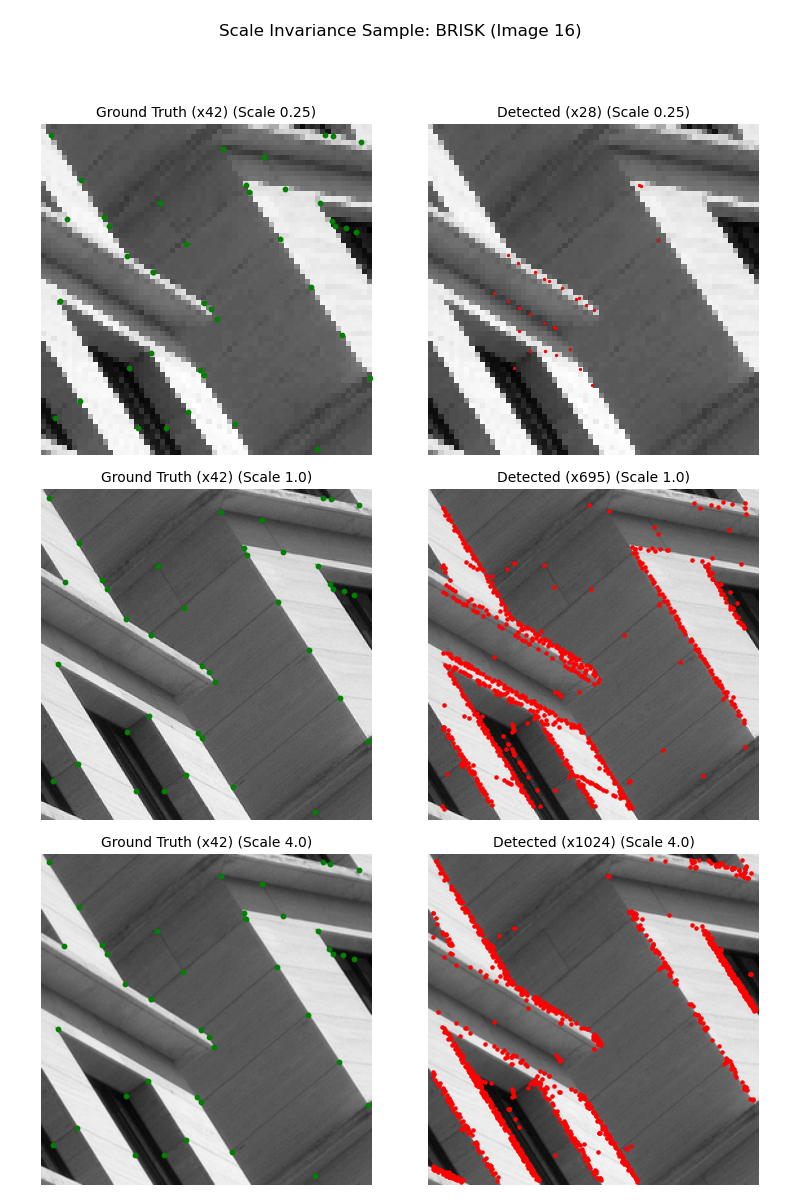
\includegraphics[width=\linewidth]{../results/scale_invariance_samples/BRISK_scale_invariance_sample.png}
    \caption{Scale invariance sample for BRISK on a randomly selected image, showing ground truth (green circles) and detected corners (red circles) at scales [0.25, 1.0, 4.0].}
    \end{minipage}
    }
\end{figure}

\begin{figure}[h]
    \centering
    \fbox{
        \begin{minipage}{0.47\textwidth}
    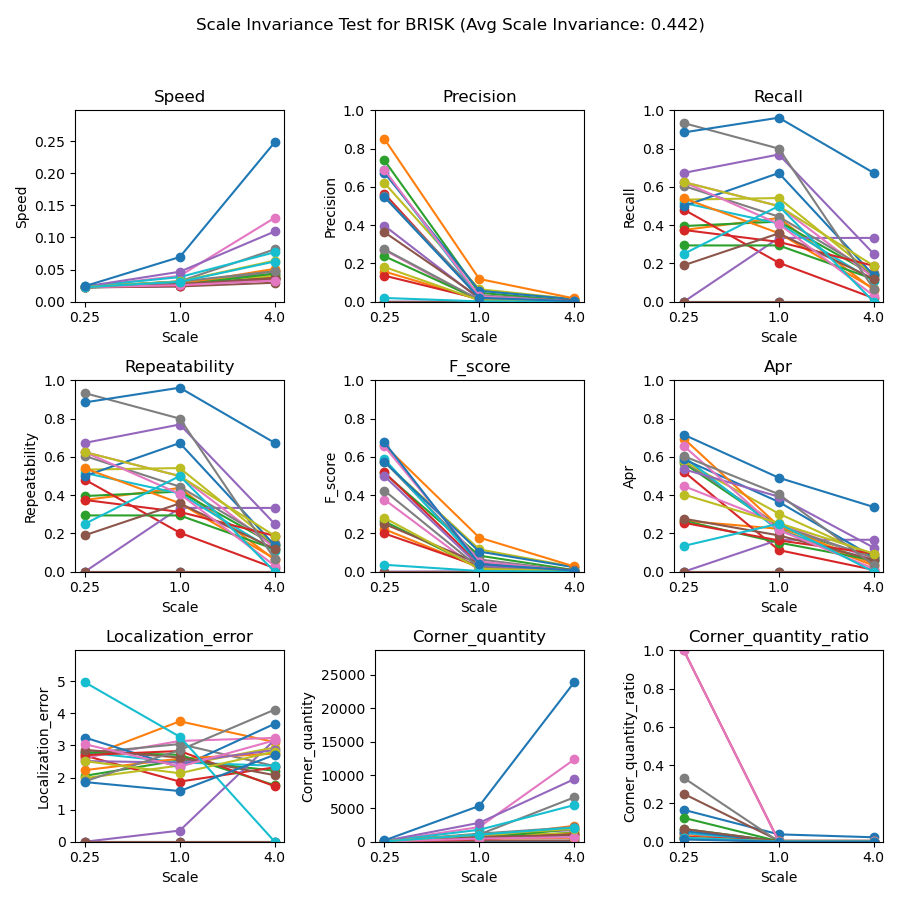
\includegraphics[width=\linewidth]{../results/scale_invariance_plots/BRISK_scale_invariance.png}
    \caption{Scale invariance results for BRISK, showing metrics across scales [0.25, 1.0, 4.0] for each image, with an average scale invariance score.}
    \end{minipage}
    }
\end{figure}

\begin{figure}[h]
\centering
\fbox{
    \begin{minipage}{0.45\textwidth}
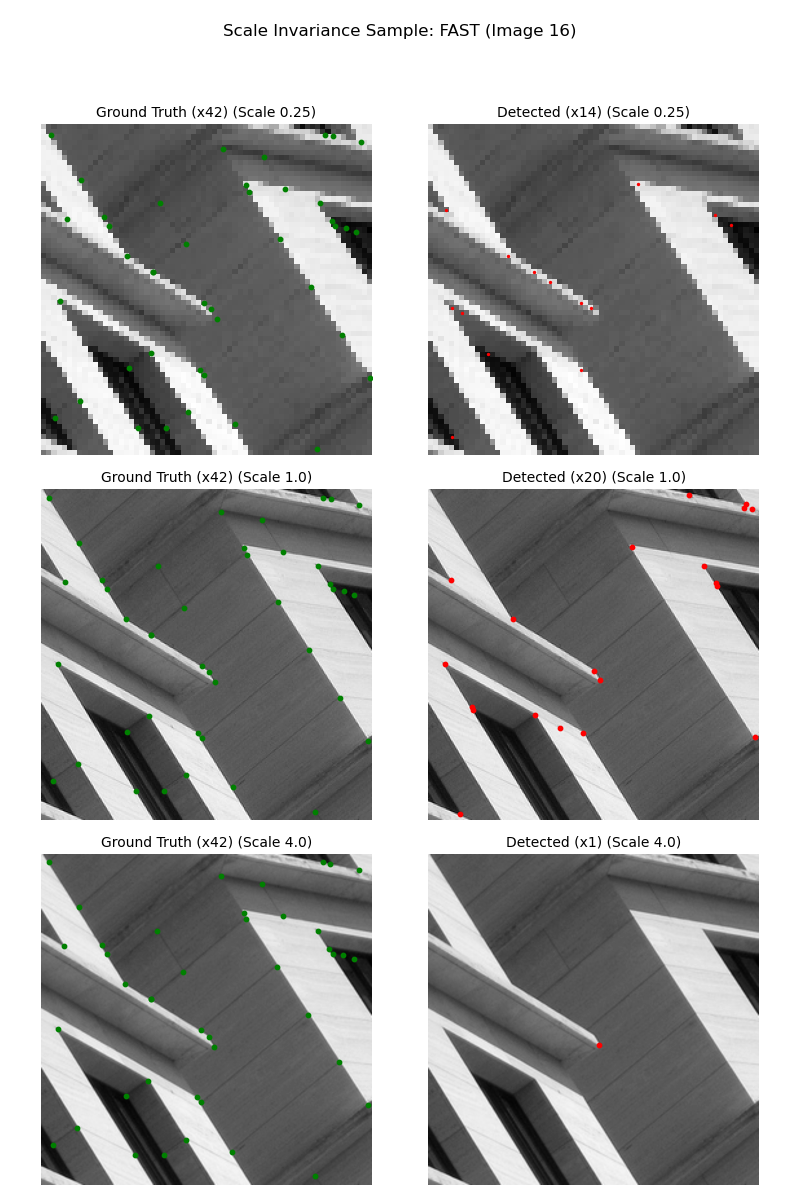
\includegraphics[width=\linewidth]{../results/scale_invariance_samples/FAST_scale_invariance_sample.png}
\caption{Scale invariance sample for FAST on a randomly selected image, showing ground truth (green circles) and detected corners (red circles) at scales [0.25, 1.0, 4.0].}
\end{minipage}
}
\end{figure}

\begin{figure}[h]
    \centering
    \fbox{
        \begin{minipage}{0.47\textwidth}
    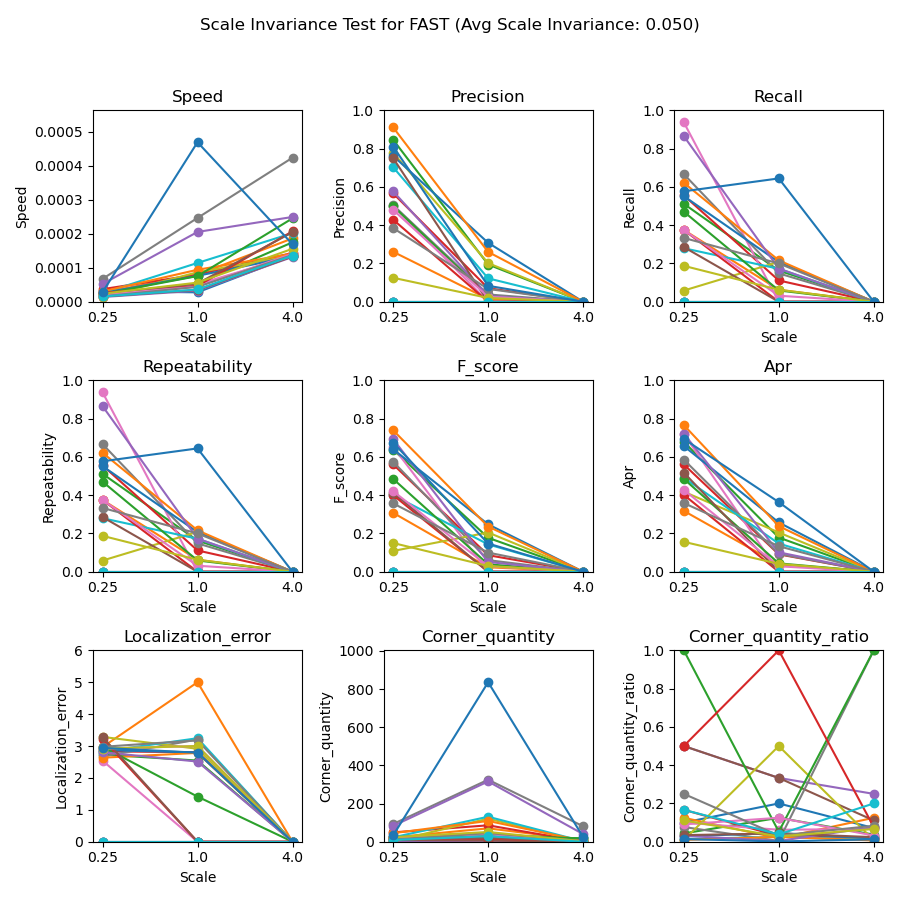
\includegraphics[width=\linewidth]{../results/scale_invariance_plots/FAST_scale_invariance.png}
    \caption{Scale invariance results for FAST, showing metrics across scales [0.25, 1.0, 4.0] for each image, with an average scale invariance score.}
    \end{minipage}
    }
\end{figure}

\begin{figure}[h]
\centering
\fbox{
    \begin{minipage}{0.47\textwidth}
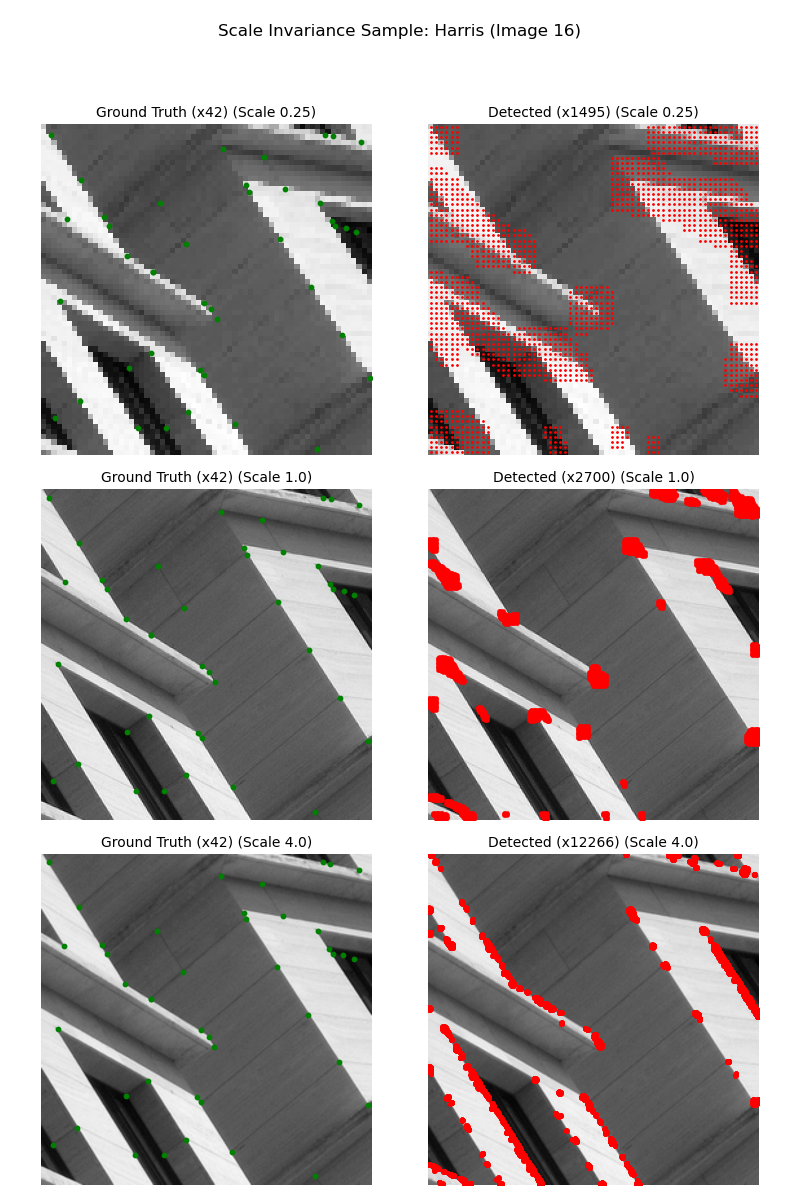
\includegraphics[width=\linewidth]{../results/scale_invariance_samples/Harris_scale_invariance_sample.png}
\caption{Scale invariance sample for Harris on a randomly selected image, showing ground truth (green circles) and detected corners (red circles) at scales [0.25, 1.0, 4.0].}
\end{minipage}
}
\end{figure}

\begin{figure}[h]
    \centering
    \fbox{
        \begin{minipage}{0.47\textwidth}
    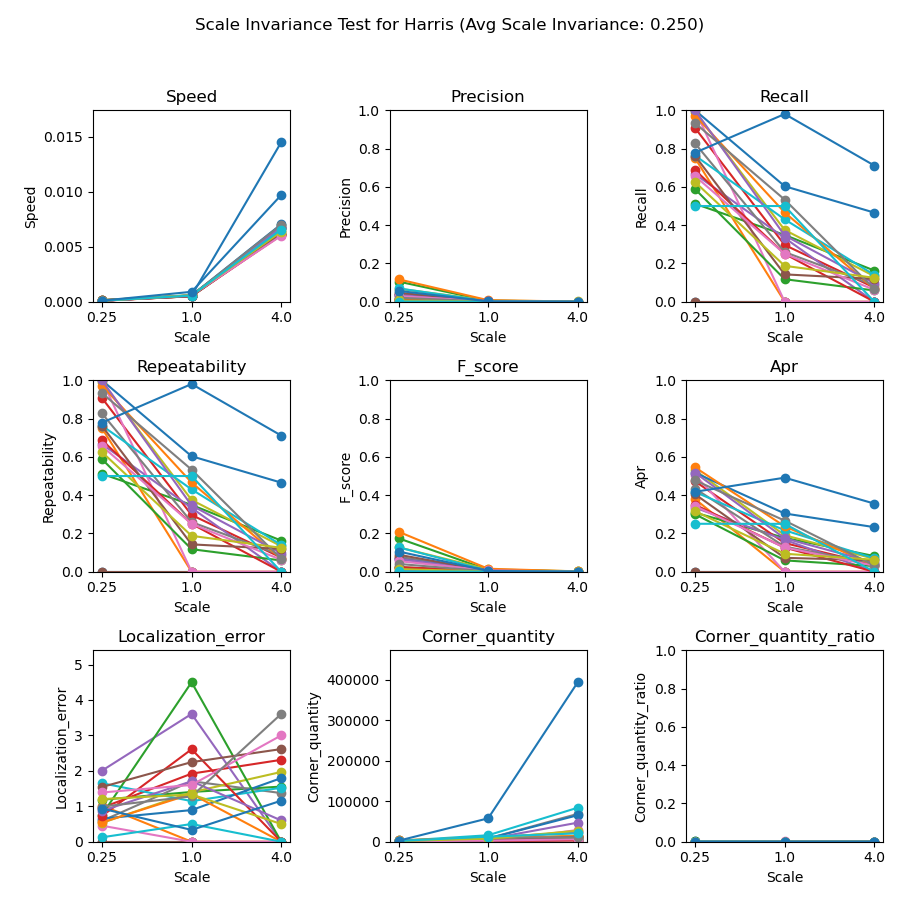
\includegraphics[width=\linewidth]{../results/scale_invariance_plots/Harris_scale_invariance.png}
    \caption{Scale invariance results for Harris, showing metrics across scales [0.25, 1.0, 4.0] for each image, with an average scale invariance score.}
    \end{minipage}
    }
\end{figure}

\begin{figure}[h]
\centering
\fbox{
    \begin{minipage}{0.47\textwidth}
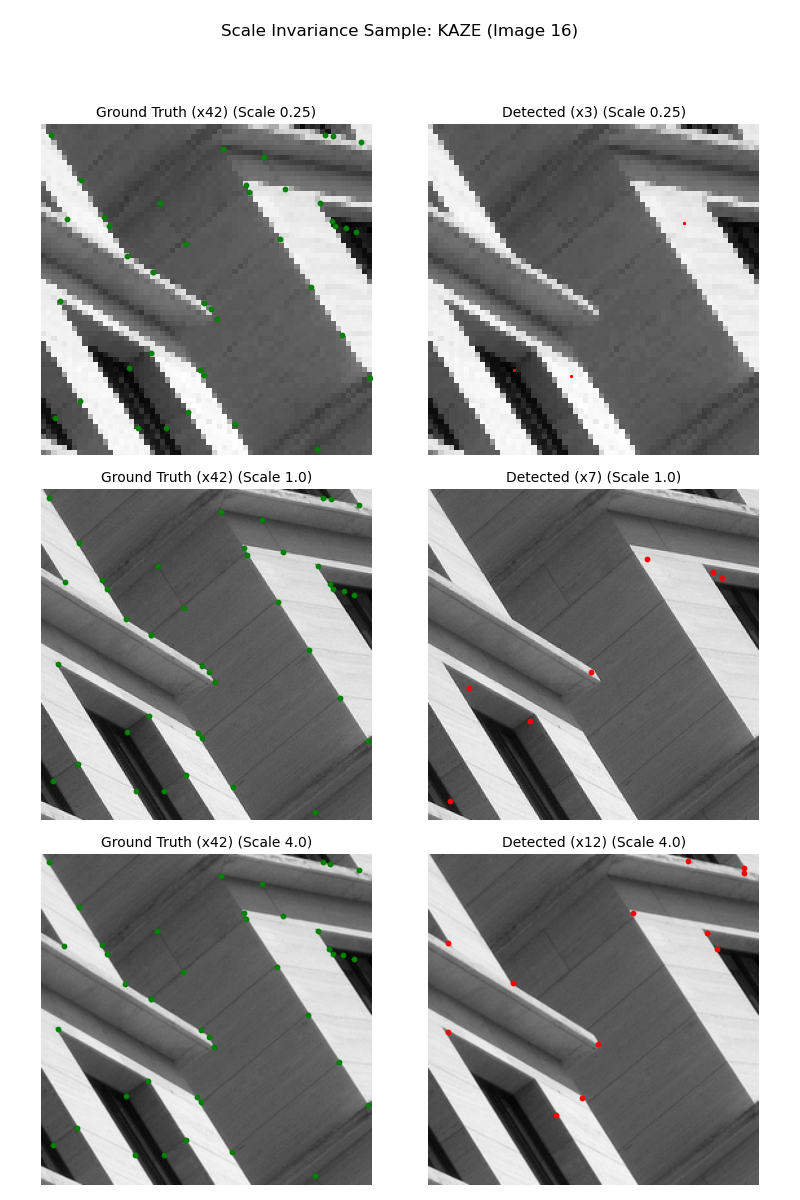
\includegraphics[width=\linewidth]{../results/scale_invariance_samples/KAZE_scale_invariance_sample.png}
\caption{Scale invariance sample for KAZE on a randomly selected image, showing ground truth (green circles) and detected corners (red circles) at scales [0.25, 1.0, 4.0].}
\end{minipage}
}
\end{figure}

\begin{figure}[h]
    \centering
    \fbox{
        \begin{minipage}{0.47\textwidth}
    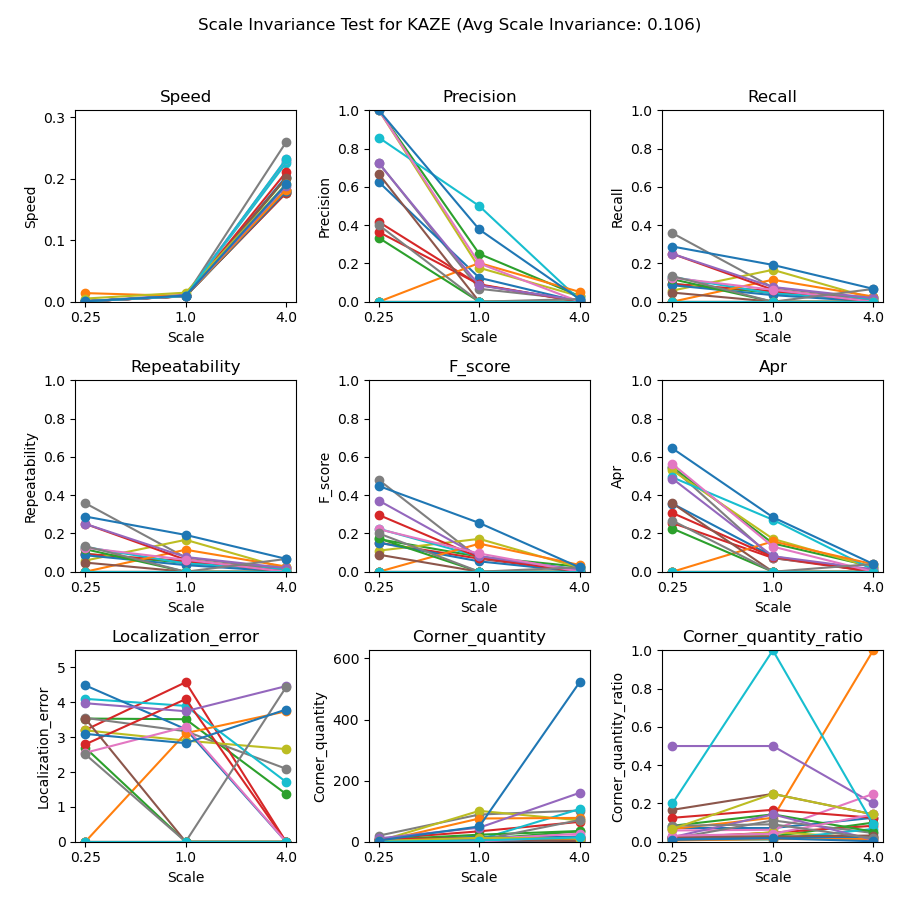
\includegraphics[width=\linewidth]{../results/scale_invariance_plots/KAZE_scale_invariance.png}
    \caption{Scale invariance results for KAZE, showing metrics across scales [0.25, 1.0, 4.0] for each image, with an average scale invariance score.}
    \end{minipage}
    }
\end{figure}

\begin{figure}[h]
\centering
\fbox{
    \begin{minipage}{0.47\textwidth}
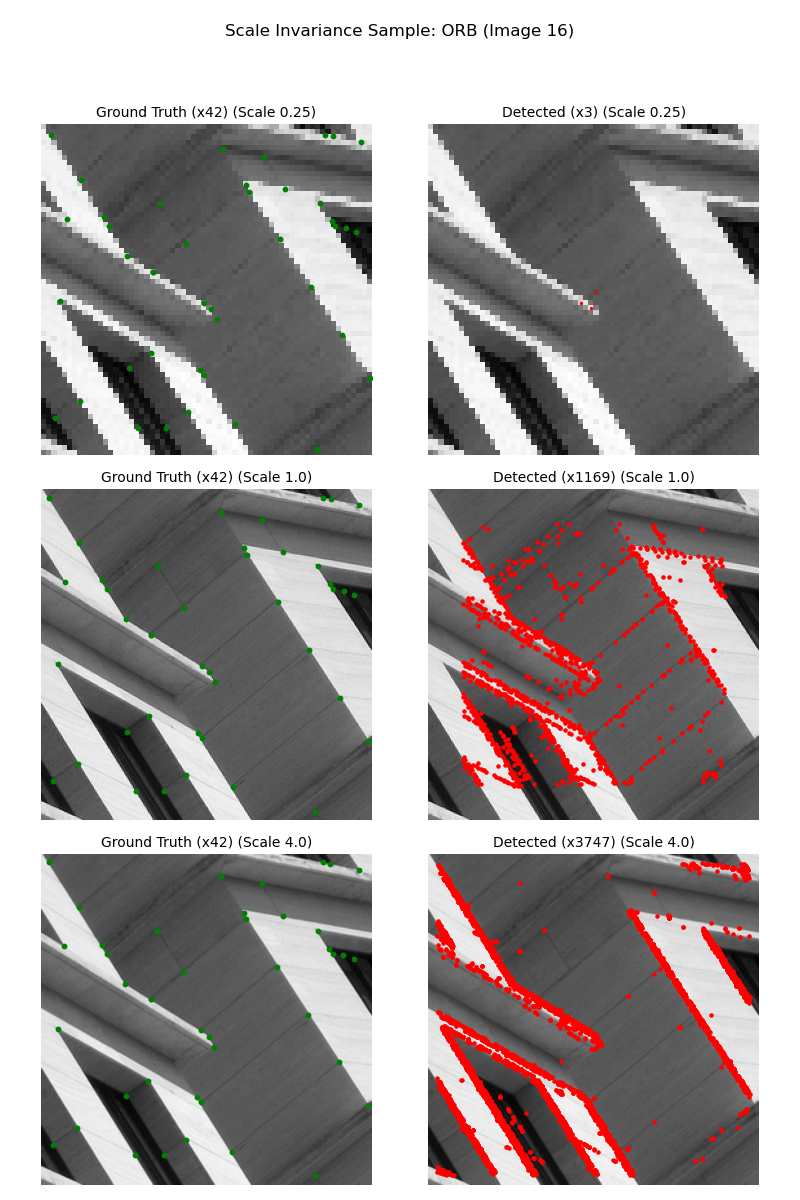
\includegraphics[width=\linewidth]{../results/scale_invariance_samples/ORB_scale_invariance_sample.png}
\caption{Scale invariance sample for ORB on a randomly selected image, showing ground truth (green circles) and detected corners (red circles) at scales [0.25, 1.0, 4.0].}
\end{minipage}
}
\end{figure}

\begin{figure}[h]
    \centering
    \fbox{
        \begin{minipage}{0.47\textwidth}
    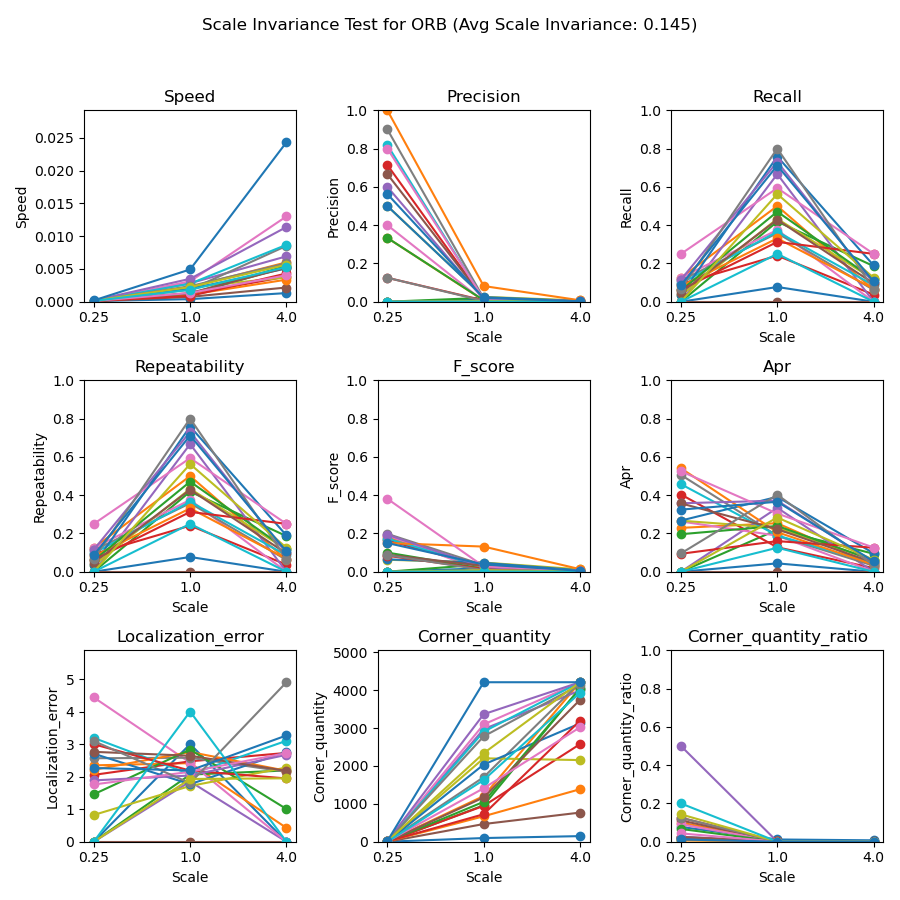
\includegraphics[width=\linewidth]{../results/scale_invariance_plots/ORB_scale_invariance.png}
    \caption{Scale invariance results for ORB, showing metrics across scales [0.25, 1.0, 4.0] for each image, with an average scale invariance score.}
    \end{minipage}
    }
\end{figure}

\begin{figure}[h]
\centering
\fbox{
    \begin{minipage}{0.47\textwidth}
\includegraphics[width=\linewidth]{../results/scale_invariance_samples/Shi-Tomasi_scale_invariance_sample.png}
\caption{Scale invariance sample for Shi-Tomasi on a randomly selected image, showing ground truth (green circles) and detected corners (red circles) at scales [0.25, 1.0, 4.0].}
\end{minipage}
}
\end{figure}

\begin{figure}[h]
    \centering
    \fbox{
        \begin{minipage}{0.47\textwidth}
    \includegraphics[width=\linewidth]{../results/scale_invariance_plots/Shi-Tomasi_scale_invariance.png}
    \caption{Scale invariance results for Shi-Tomasi, showing metrics across scales [0.25, 1.0, 4.0] for each image, with an average scale invariance score.}
    \end{minipage}
    }
\end{figure}

\begin{figure}[h]
\centering
\fbox{
    \begin{minipage}{0.47\textwidth}
\includegraphics[width=\linewidth]{../results/scale_invariance_samples/SIFT_scale_invariance_sample.png}
\caption{Scale invariance sample for Sift on a randomly selected image, showing ground truth (green circles) and detected corners (red circles) at scales [0.25, 1.0, 4.0].}
\end{minipage}
}
\end{figure}

\begin{figure}[h]
    \centering
    \fbox{
        \begin{minipage}{0.47\textwidth}
    \includegraphics[width=\linewidth]{../results/scale_invariance_plots/SIFT_scale_invariance.png}
    \caption{Scale invariance results for SIFT, showing metrics across scales [0.25, 1.0, 4.0] for each image, with an average scale invariance score.}
    \end{minipage}
    }
\end{figure}


%%%%%%%%%%%%%%%%%%%%%%%%%%%%%%%%%%%%%%%%%%%%%%%%%%%%%%%%%%%%%%%%%%%%%%%%%%%%%%%%%%%%%%%%%%%

%%%%%%%%%%%%%%%%%%%%%%%%%%%%%%%%%%%%%%%%%%%%%%%%%%%%%%%%%%%%%%%%%%%%%%%%%%%%%%%%%%%%%%%%%%%%

\onecolumn
\section{All Developed Python Code}
\label{app:code}

\begin{lstlisting}[style=python, caption={Driver Script for Project}, label={lst:driver}]
## import standard libraries
import numpy as np
import cv2
import os
import time
import itertools
from tqdm import tqdm
import re
import random

## import custom scripts
import corner_methods as cm
from parameters import ALGORITHMS, PARAM_GRIDS, image_path, ground_truth_path, output_path, SCALES, N_SAMPLES, MAX_SAMPLES, SEED
import utilities as utils
from distributions import sample_param_grid

def get_ground_truth(image_path, ground_truth_path, output_path, images=None, image_names=None, ground_truth_corners=None):
    
    images = images or []
    image_names = image_names or []
    ground_truth_corners = ground_truth_corners or []
    
    sorted_files = sorted(os.listdir(image_path), key=lambda x: int(re.search(r'\d+', x).group()))
    
    ## read in images and truth points
    for image in sorted_files:
        corners = f"{image.split('.')[0]}.txt"
        image_names.append(image.split('.')[0])
        images.append(cv2.imread(os.path.join(image_path, image), cv2.IMREAD_GRAYSCALE))
        
        with open(os.path.join(ground_truth_path, corners), 'r') as file:
            coordinate_pairs = np.array([tuple(map(int, line.split())) for line in file])
        ground_truth_corners.append(coordinate_pairs)
        

    if not os.path.isdir(output_path):
        os.makedirs(output_path)
    utils.plot_ground_truth(images, image_names, ground_truth_corners, output_path)
    
    return images, image_names, ground_truth_corners

def optimize_across_images(algorithm, alg_name, images, gt_corners_list, param_grid):

    best_params = {}
    best_score = -1

    param_names, param_values = sample_param_grid(param_grid, N_SAMPLES)
    total_combinations = np.prod([len(values) for values in param_values])
    
    # Limit to a maximum number of combinations
    param_combinations = list(itertools.product(*param_values))
    if MAX_SAMPLES:
        if len(param_combinations) > MAX_SAMPLES:
            param_combinations = random.sample(param_combinations, MAX_SAMPLES)
            total_combinations = MAX_SAMPLES
    
    # Store metrics for each parameter combination
    all_metrics = []
    
    # Use tqdm to show progress with total combinations
    for combo in tqdm(param_combinations, total=total_combinations, desc=f"Optimizing {total_combinations} Runs: {alg_name}"):
        params = dict(zip(param_names, combo))
        speeds = []
        precisions = []
        recalls = []
        repeatabilities = []
        f_scores = []
        aprs = []
        localization_errors = []
        corner_quantities = []
        corner_quantity_ratios = []
        
        for image, gt_corners in zip(images, gt_corners_list):
            start_time = time.time()
            corners = algorithm(image, args=params)
            exec_time = time.time() - start_time
            precision, recall, repeatability, f_score, apr, localization_error, corner_quantity, corner_quantity_ratio = utils.calculate_metrics(corners, gt_corners)
            
            speeds.append(exec_time)
            precisions.append(precision)
            recalls.append(recall)
            repeatabilities.append(repeatability)
            f_scores.append(f_score)
            aprs.append(apr)
            localization_errors.append(localization_error)
            corner_quantities.append(corner_quantity)
            corner_quantity_ratios.append(corner_quantity_ratio)
            
        # Normalize speed to [0, 1] for scoring (lower speed is better, so invert it)
        speed_norm = np.max(speeds) if speeds else 1.0
        if speed_norm > np.mean(speeds) + 4 * np.std(speeds):
            speed_norm = np.mean(speeds) + 4 * np.std(speeds)
        normalized_speeds = [1 - (speed / speed_norm) if speed_norm > 0 else 1.0 for speed in speeds]
        
        # Normalize localization error to [0, 1] for scoring (lower is better, so invert it)
        max_le = np.max(localization_errors) if localization_errors and np.max(localization_errors) > 0 else 1.0
        normalized_le = [1 - (le / max_le) if max_le > 0 else 1.0 for le in localization_errors]
        
        # Compute average metrics
        avg_speed = np.mean(normalized_speeds)
        avg_precision = np.mean(precisions)
        avg_recall = np.mean(recalls)
        avg_repeatability = np.mean(repeatabilities)
        avg_f_score = np.mean(f_scores)
        avg_apr = np.mean(aprs)
        avg_le = np.mean(normalized_le)
        avg_corner_quant = np.mean(corner_quantity)
        avg_corner_quant_ratios = np.mean(corner_quantity_ratios)
        
        # Score is the average of the normalized metrics (excluding corner_quantity since it's not part of optimization)
        # weights = np.array([2/12, 3/12, 3/12, 1/12, 2/12, 1/12])
        vars = np.array([avg_speed, avg_precision, avg_recall, avg_le, avg_corner_quant_ratios]) #avg_repeatability
        # score = np.sum(vars * weights)
        score = np.sum(vars) / len(vars)
        
        # Store metrics for this combination
        all_metrics.append({
            'params': params,
            'speed': speeds,
            'precision': precisions,
            'recall': recalls,
            'repeatability': repeatabilities,
            'f_score': f_scores,
            'apr': aprs,
            'localization_error': localization_errors,
            'corner_quantity': corner_quantities,
            'corner_quantity_ratio': corner_quantity_ratios,
            'score': score
        })
        
        if score > best_score:
            best_score = score
            best_params = params
    
    return best_params, best_score, total_combinations, all_metrics

def test_scale_invariance(images, image_names, ground_truth_corners, optimized_params):

    scale_results = {name: {img_name: {
        'speed': [], 'precision': [], 'recall': [], 'repeatability': [], 'f_score': [], 'apr': [],
        'localization_error': [], 'corner_quantity': [], 'corner_quantity_ratio': [], 'scale_invariance': 0.0
    } for img_name in image_names} for name in ALGORITHMS}
        
    # Select a random image for sample visualization
    sample_idx = np.random.randint(0, len(images))
    sample_image = images[sample_idx]
    sample_name = image_names[sample_idx]
    sample_gt_corners = ground_truth_corners[sample_idx]
    
    for alg_name, alg_func in tqdm(ALGORITHMS.items(), desc="Testing Scale Invariance"):
        best_params = optimized_params[alg_name]
        scaled_images = utils.create_scaled_images(sample_image)
        sample_corners = []
        
        for img_idx, (image, gt_corners, name) in enumerate(zip(images, ground_truth_corners, image_names)):
            scaled_images_current = utils.create_scaled_images(image)
            repeatabilities = []  # To compute scale invariance
            
            for scale_idx, scaled_img in enumerate(scaled_images_current):
                start_time = time.time()
                corners = alg_func(scaled_img, args=best_params)
                exec_time = time.time() - start_time
                
                # Adjust ground truth for scale
                scaled_gt = gt_corners * SCALES[scale_idx]
                
                precision, recall, repeatability, f_score, apr, localization_error, corner_quantity, corner_quantity_ratio = utils.calculate_metrics(corners, scaled_gt)
                
                # Store results for this scale
                scale_results[alg_name][name]['speed'].append(exec_time)
                scale_results[alg_name][name]['precision'].append(precision)
                scale_results[alg_name][name]['recall'].append(recall)
                scale_results[alg_name][name]['repeatability'].append(repeatability)
                scale_results[alg_name][name]['f_score'].append(f_score)
                scale_results[alg_name][name]['apr'].append(apr)
                scale_results[alg_name][name]['localization_error'].append(localization_error)
                scale_results[alg_name][name]['corner_quantity'].append(corner_quantity)
                scale_results[alg_name][name]['corner_quantity_ratio'].append(corner_quantity_ratio)
                
                repeatabilities.append(repeatability)
                
                # Store corners for the sample image
                if img_idx == sample_idx:
                    sample_corners.append(corners)
            
            # Compute scale invariance as 1 - coefficient of variation of repeatability
            repeatabilities = np.array(repeatabilities)
            if repeatabilities.mean() > 0:
                cv = repeatabilities.std() / repeatabilities.mean()
                scale_invariance = max(0, min(1, 1 - cv))  # Higher value = better scale invariance
            else:
                scale_invariance = 0.0
            
            scale_results[alg_name][name]['scale_invariance'] = scale_invariance
        
        # Generate sample visualization for this algorithm
        utils.generate_scale_invariance_samples(
            scaled_images, sample_corners, sample_gt_corners, 
            alg_name, sample_name, output_path
        )
    
    return scale_results

def run_benchmarking(images, image_names, ground_truth_corners):

    results = {name: {
        'speed': [], 'precision': [], 'recall': [], 'repeatability': [], 'f_score': [], 'apr': [],
        'localization_error': [], 'corner_quantity': [], 'corner_quantity_ratio': []
    } for name in ALGORITHMS}
    individual_results = {name: {img_name: {
        'speed': [], 'precision': [], 'recall': [], 'repeatability': [], 'f_score': [], 'apr': [],
        'localization_error': [], 'corner_quantity': [], 'corner_quantity_ratio': []
    } for img_name in image_names} for name in ALGORITHMS}
    optimized_params = {}
    all_metrics_per_algorithm = {}  # Store all metrics for each parameter combination per algorithm
    
    # Optimize parameters and benchmark for each algorithm
    params = []
    combinations = []
    scores = []
    
    for alg_name, alg_func in tqdm(ALGORITHMS.items(), desc="Generating Optimization Data"):
        # Optimize parameters across all images and store all metrics
        best_params, best_score, total_combinations, all_metrics = optimize_across_images(alg_func, alg_name, images, ground_truth_corners, PARAM_GRIDS[alg_name])
        params.append(best_params)
        combinations.append(total_combinations)
        scores.append(best_score)
        optimized_params[alg_name] = best_params
        all_metrics_per_algorithm[alg_name] = all_metrics
        
        # Benchmark with optimized parameters for this algorithm
        for img_idx, (image, gt_corners, name) in enumerate(zip(images, ground_truth_corners, image_names)):
            start_time = time.time()
            corners = alg_func(image, args=best_params)
            exec_time = time.time() - start_time
            
            precision, recall, repeatability, f_score, apr, localization_error, corner_quantity, corner_quantity_ratio = utils.calculate_metrics(corners, gt_corners)
            
            # Store aggregated results
            results[alg_name]['speed'].append(exec_time)
            results[alg_name]['precision'].append(precision)
            results[alg_name]['recall'].append(recall)
            results[alg_name]['repeatability'].append(repeatability)
            results[alg_name]['f_score'].append(f_score)
            results[alg_name]['apr'].append(apr)
            results[alg_name]['localization_error'].append(localization_error)
            results[alg_name]['corner_quantity'].append(corner_quantity)
            results[alg_name]['corner_quantity_ratio'].append(corner_quantity_ratio)
            
            # Store individual results
            individual_results[alg_name][name]['speed'].append(exec_time)
            individual_results[alg_name][name]['precision'].append(precision)
            individual_results[alg_name][name]['recall'].append(recall)
            individual_results[alg_name][name]['repeatability'].append(repeatability)
            individual_results[alg_name][name]['f_score'].append(f_score)
            individual_results[alg_name][name]['apr'].append(apr)
            individual_results[alg_name][name]['localization_error'].append(localization_error)
            individual_results[alg_name][name]['corner_quantity'].append(corner_quantity)
            individual_results[alg_name][name]['corner_quantity_ratio'].append(corner_quantity_ratio)
    
    return results, optimized_params, individual_results, params, combinations, scores, all_metrics_per_algorithm

if __name__ == "__main__":

    np.random.seed(SEED)
    
    print("Loading Ground Truth ...")
    images, image_names, ground_truth_corners = get_ground_truth(image_path, ground_truth_path, output_path)
    results, optimized_params, individual_results, params, combinations, scores, all_metrics_per_algorithm = run_benchmarking(images, image_names, ground_truth_corners)

    # Generate sample detection images with optimized parameters
    print("Creating Sample Imagery for Optimized Algorithms ...")
    utils.generate_sample_detections(images, image_names, ground_truth_corners, optimized_params, output_path)
    
    # Save results
    print("Writing Results Files ...")
    os.makedirs(output_path, exist_ok=True)
    os.makedirs(os.path.join(output_path, "data"), exist_ok=True)
    for alg_name in results:
        np.savez(os.path.join(output_path, f'data/{alg_name}_results.npz'), **results[alg_name])
        for img_name in image_names:
            np.savez(os.path.join(output_path, f'data/{alg_name}_{img_name}_individual_results.npz'), **individual_results[alg_name][img_name])
    
    # Generate comparison tables and reports
    utils.generate_param_report(params, combinations, scores, output_path)
    utils.generate_comparison_tables(results, output_path)
    
    # Generate individual result plots and pairwise metric plots
    print("Plotting Result Images ...")
    utils.visualize_results(output_path, image_names)
    # utils.plot_pairwise_metrics(results, output_path)
    utils.plot_best_combination(individual_results, image_names, output_path)
    utils.plot_all_combinations(all_metrics_per_algorithm, image_names, output_path)
    
    # Run scale invariance test
    scale_results = test_scale_invariance(images, image_names, ground_truth_corners, optimized_params)
    utils.plot_scale_invariance(scale_results, image_names, output_path)
    utils.generate_scale_invariance_table(scale_results, output_path)
    
    utils.plot_all_detections(images, image_names, optimized_params, output_path)
\end{lstlisting}
\bigskip
\bigskip

\begin{lstlisting}[style=python, caption={Setup Parameters}, label={lst:params}]
from corner_methods import *
import os
from distributions import UniformDist, NormalDist, CategoricalDist

image_path = os.path.join(os.getcwd(), "data/Urban_Corner_datasets/Images")
ground_truth_path = os.path.join(os.getcwd(), "data/Urban_Corner_datasets/Ground_Truth")
output_path = os.path.join(os.getcwd(), "results")

SCALES = [0.25, 1.0, 4.0]  # Scales to test

N_SAMPLES = 20
MAX_SAMPLES = 250
SEED = 11003

ALGORITHMS = {
                'Harris'    : harris,
                'Shi-Tomasi': shi_tomasi,
                'FAST'      : fast,
                'ORB'       : orb,
                'SIFT'      : sift,
                'BRISK'     : brisk,
                'AGAST'     : agast,
                'KAZE'      : kaze,
                'AKAZE'     : akaze
            }

## Using custom distribution generation code
PARAM_GRIDS = {
    'Harris': {
        'blockSize': UniformDist(min_val=2, max_val=11, is_int=True),
        'ksize': CategoricalDist(options=[3, 5, 7, 9, 11]),  # Only odd integers
        'k': UniformDist(min_val=0.01, max_val=0.15),
        'borderType': CategoricalDist(options=[
            cv2.BORDER_DEFAULT, cv2.BORDER_CONSTANT, cv2.BORDER_REFLECT
        ])
    },
    # ... (rest of PARAM_GRIDS unchanged)
    'Shi-Tomasi': {
        'maxCorners': UniformDist(min_val=25, max_val=1000, is_int=True),
        'qualityLevel': UniformDist(min_val=0.005, max_val=0.2),
        'minDistance': UniformDist(min_val=3, max_val=30, is_int=True),
        'blockSize': UniformDist(min_val=3, max_val=9, is_int=True)
    },
    'FAST': {
        'threshold': UniformDist(min_val=5, max_val=100, is_int=True),
        'type': CategoricalDist(options=[
            cv2.FAST_FEATURE_DETECTOR_TYPE_5_8,
            cv2.FAST_FEATURE_DETECTOR_TYPE_7_12,
            cv2.FAST_FEATURE_DETECTOR_TYPE_9_16
        ])
    },
    'ORB': {
        'nfeatures': UniformDist(min_val=100, max_val=5000, is_int=True),
        'scaleFactor': UniformDist(min_val=1.05, max_val=1.5),
        'nlevels': UniformDist(min_val=4, max_val=16, is_int=True),
        'edgeThreshold': UniformDist(min_val=15, max_val=70, is_int=True),
        'patchSize': UniformDist(min_val=15, max_val=50, is_int=True),
        'fastThreshold': UniformDist(min_val=5, max_val=100, is_int=True)
    },
    'SIFT': {
        'nOctaveLayers': UniformDist(min_val=2, max_val=6, is_int=True),
        'contrastThreshold': UniformDist(min_val=0.02, max_val=0.16),
        'edgeThreshold': UniformDist(min_val=5, max_val=30, is_int=True),
        'sigma': NormalDist(mean=1.6, std=0.4, min_val=1.0, max_val=2.4)
    },
    'BRISK': {
        'thresh': UniformDist(min_val=10, max_val=100, is_int=True),
        'octaves': UniformDist(min_val=2, max_val=6, is_int=True),
        'patternScale': UniformDist(min_val=0.5, max_val=2.0)
    },
    'AGAST': {
        'threshold': UniformDist(min_val=5, max_val=50, is_int=True),
        'type': CategoricalDist(options=[
            cv2.AgastFeatureDetector_AGAST_5_8,
            cv2.AgastFeatureDetector_AGAST_7_12d,
            cv2.AgastFeatureDetector_OAST_9_16
        ])
    },
    'KAZE': {
        'threshold': UniformDist(min_val=0.0005, max_val=0.004),
        'nOctaves': UniformDist(min_val=2, max_val=6, is_int=True),
        'nOctaveLayers': UniformDist(min_val=2, max_val=6, is_int=True),
        'diffusivity': CategoricalDist(options=[
            cv2.KAZE_DIFF_PM_G1, cv2.KAZE_DIFF_PM_G2, cv2.KAZE_DIFF_WEICKERT
        ])
    },
    'AKAZE': {
        'threshold': UniformDist(min_val=0.0005, max_val=0.004),
        'nOctaves': UniformDist(min_val=3, max_val=6, is_int=True),
        'nOctaveLayers': UniformDist(min_val=2, max_val=6, is_int=True),
        'diffusivity': CategoricalDist(options=[
            cv2.KAZE_DIFF_PM_G1, cv2.KAZE_DIFF_PM_G2
        ])
    }
}

PARAM_REPORT = [
    "\\begin{table}[h]",
    "\\centering",
    "\\small",
    "\\caption{Optimal Parameters for Corner Detection Algorithms}",
    "\\label{tab:optimal_parameters}",
    "\\begin{tabular}{lp{3.5cm}cc}",
    "\\toprule",
    "\\textbf{Algorithm} & \\textbf{Optimal Parameters} & \\textbf{$\\#$ Tests} & \\textbf{Best Score} \\\\",
    "\\midrule"
]
\end{lstlisting}
\bigskip
\bigskip

\begin{lstlisting}[style=python, caption={Random Variable Distribution Setup}, label={lst:distributions}]
import numpy as np

class UniformDist:
    def __init__(self, min_val, max_val, is_int=False):
        self.min_val = min_val
        self.max_val = max_val
        self.is_int = is_int

    def sample(self, n_samples):
        samples = np.round(np.random.uniform(self.min_val, self.max_val, n_samples), 4)
        if self.is_int:
            samples = np.round(samples).astype(int)
            samples = np.clip(samples, self.min_val, self.max_val)
            
        return np.unique(samples)[:n_samples]  # Ensure unique samples

class NormalDist:
    def __init__(self, mean, std, min_val=None, max_val=None, is_int=False):
        self.mean = mean
        self.std = std
        self.min_val = min_val
        self.max_val = max_val
        self.is_int = is_int

    def sample(self, n_samples):
        samples = np.random.normal(self.mean, self.std, n_samples)
        if self.min_val is not None or self.max_val is not None:
            samples = np.round(np.clip(samples, self.min_val or -np.inf, self.max_val or np.inf), 4)
        if self.is_int:
            samples = np.round(samples).astype(int)
            samples = np.clip(samples, self.min_val or -np.inf, self.max_val or np.inf)
        return np.unique(samples)[:n_samples]

class CategoricalDist:
    def __init__(self, options):
        self.options = options

    def sample(self, n_samples):
        if n_samples <= len(self.options):
            return np.random.choice(self.options, n_samples, replace=False)
        else:
            return np.random.choice(self.options, n_samples, replace=True)

    
def sample_param_grid(param_grid, n_samples):

    sampled_grid = {}
    for param_name, dist in param_grid.items():
        sampled_grid[param_name] = dist.sample(n_samples)
    return list(sampled_grid.keys()), list(sampled_grid.values())
\end{lstlisting}
\bigskip
\bigskip

\begin{lstlisting}[style=python, caption={All Corner Detection Wrappers}, label={lst:corner_methods}]
import cv2
import numpy as np

def harris(image, args=None):

    args = args or {'blockSize': 2, 'ksize': 3, 'k': 0.04}
    corners = cv2.cornerHarris(image, **args)
    corners = cv2.dilate(corners, None)
    corners = np.column_stack(np.where(corners > 0.01 * corners.max()))
    return corners[:, ::-1].astype(np.float32)

def shi_tomasi(image, args=None):

    args = args or {'maxCorners': 25, 'qualityLevel': 0.01, 'minDistance': 10}
    corners = cv2.goodFeaturesToTrack(image, **args)
    return corners[:, 0].astype(np.float32) if corners is not None else np.array([])

def fast(image, args=None):

    args = args or {'threshold': 25, 'type': cv2.FAST_FEATURE_DETECTOR_TYPE_7_12}
    fast = cv2.FastFeatureDetector_create(nonmaxSuppression=True, **args)
    keypoints = fast.detect(image, None)
    return np.array([kp.pt for kp in keypoints], dtype=np.float32)

def orb(image, args=None):

    args = args or {
        'nfeatures': 500, 'scaleFactor': 1.1, 'nlevels': 10,
        'edgeThreshold': 31, 'firstLevel': 0, 'WTA_K': 2,
        'scoreType': cv2.ORB_HARRIS_SCORE, 'patchSize': 31, 'fastThreshold': 20
    }
    orb = cv2.ORB_create(**args)
    keypoints = orb.detect(image, None)
    return np.array([kp.pt for kp in keypoints], dtype=np.float32)

def sift(image, args=None):

    args = args or {
        'nOctaveLayers': 3, 'contrastThreshold': 0.04, 'edgeThreshold': 10, 'sigma': 1.6
    }
    sift = cv2.SIFT_create(**args)
    keypoints, _ = sift.detectAndCompute(image, None)
    return np.array([kp.pt for kp in keypoints], dtype=np.float32)

def brisk(image, args=None):

    args = args or {'thresh': 30, 'octaves': 3, 'patternScale': 1.0}
    brisk = cv2.BRISK_create(**args)
    keypoints, _ = brisk.detectAndCompute(image, None)
    return np.array([kp.pt for kp in keypoints], dtype=np.float32)

def agast(image, args=None):

    args = args or {'threshold': 10, 'type': 1}
    agast = cv2.AgastFeatureDetector_create(nonmaxSuppression=True, **args)
    keypoints = agast.detect(image, None)
    return np.array([kp.pt for kp in keypoints], dtype=np.float32)

def kaze(image, args=None):

    args = args or {'threshold': 0.001, 'nOctaves': 3, 'nOctaveLayers': 3, 'diffusivity': 1}
    kaze = cv2.KAZE_create(**args)
    keypoints, _ = kaze.detectAndCompute(image, None)
    return np.array([kp.pt for kp in keypoints], dtype=np.float32)

def akaze(image, args=None):

    args = args or {'threshold': 0.001, 'nOctaves': 4, 'nOctaveLayers': 4, 'diffusivity': 2}
    akaze = cv2.AKAZE_create(**args)
    keypoints, _ = akaze.detectAndCompute(image, None)
    return np.array([kp.pt for kp in keypoints], dtype=np.float32)
\end{lstlisting}
\bigskip
\bigskip

\begin{lstlisting}[style=python, caption={Utility Functions for Data Processing}, label={lst:utilities}]
import numpy as np
import cv2
from itertools import product
import matplotlib.pyplot as plt
import os
from scipy.spatial.distance import cdist
from tqdm import tqdm
from parameters import PARAM_REPORT, ALGORITHMS, SCALES


def plot_ground_truth(images, image_names, ground_truth_corners, output_path):
    
    plt.figure(figsize=(8,10))
    plt.suptitle("Ground Truth Images")
    for i in range(len(images)):
        plt.subplot(6, 4, i+1)
        plt.imshow(images[i], cmap="gray")
        plt.axis("off")
        plt.title(f"Image {image_names[i]} (x{len(ground_truth_corners[i])})")
        for corner in ground_truth_corners[i]:
            plt.scatter(corner[1], corner[0], color="green", marker='o', s=10)
            
    plt.tight_layout()
    plt.savefig(os.path.join(output_path, "ground_truth.png"))
    plt.close()


def create_scaled_images(image):
    scaled_images = []
    for scale in SCALES:
        scaled = cv2.resize(image, None, fx=scale, fy=scale, interpolation=cv2.INTER_LINEAR)
        scaled_images.append(scaled)
    return scaled_images


def calculate_metrics(pred_corners, gt_corners, threshold=5.0):
    gt = np.array(gt_corners, dtype=np.float32)
    pred = np.array(pred_corners, dtype=np.float32)

    # Reshape if necessary
    if pred.ndim == 1 and pred.shape[0] == 2:
        pred = pred.reshape(1, 2)
    if pred.ndim == 1 or pred.size == 0:
        pred = np.empty((0, 2), dtype=np.float32)

    if gt.ndim == 1 and gt.shape[0] == 2:
        gt = gt.reshape(1, 2)
    if gt.ndim == 1 or gt.size == 0:
        gt = np.empty((0, 2), dtype=np.float32)

    # Overall corner quantity (total number of detected corners)
    corner_quantity = len(pred)
    corner_quantity_ratio = 1 / (np.abs(len(pred) - len(gt_corners)) + 1) ## 1/(|gt - pred| + 1)
    # Early return if either side has no corners
    if len(gt) == 0 or len(pred) == 0:
        return 0.0, 0.0, 0.0, 0.0, 0.0, 0.0, corner_quantity, corner_quantity_ratio

    # Compute distances between ground truth and predicted corners
    dists = cdist(gt, pred)  # shape: (num_gt, num_pred)
    matched_gt = np.any(dists <= threshold, axis=1)
    matched_pred = np.any(dists <= threshold, axis=0)

    TP = np.sum(matched_gt)
    FP = len(pred) - np.sum(matched_pred)
    FN = len(gt) - TP

    precision = TP / (TP + FP) if (TP + FP) > 0 else 0
    recall = TP / (TP + FN) if (TP + FN) > 0 else 0
    repeatability = TP / len(gt) if len(gt) > 0 else 0

    denom = (precision + recall)
    f_score = 2 * (precision * recall) / denom if denom > 0 else 0
    apr = (precision + recall) / 2  # Arithmetic Mean of Precision and Recall

    # Compute localization error for matched corners
    localization_error = 0.0
    if TP > 0:
        # Find the closest predicted corner for each ground truth corner
        min_dists = np.min(dists, axis=1)  # Minimum distance for each ground truth corner
        matched_dists = min_dists[matched_gt]  # Distances for matched ground truth corners
        localization_error = np.mean(matched_dists) if len(matched_dists) > 0 else 0.0

    return precision, recall, repeatability, f_score, apr, localization_error, corner_quantity, corner_quantity_ratio

        
def generate_sample_detections(images, image_names, ground_truth_corners, optimized_params, output_path):

    sample_output_path = os.path.join(output_path, "sample_detections")
    os.makedirs(sample_output_path, exist_ok=True)
    
    idx = np.random.randint(0, len(images))
    image = images[idx]
    name = image_names[idx]
    
    for alg_name, alg_func in ALGORITHMS.items():
        params = optimized_params[alg_name]
        corners = alg_func(image, args=params)
        gt_corners = ground_truth_corners[idx]
        
        plt.figure(figsize=(4, 8))  # Adjusted for 1x2 grid
        plt.suptitle(f"Sample Detection: {alg_name} (Image {name})", fontsize=12)
        
        # Ground truth subplot (left column)
        plt.subplot(2, 1, 1)
        plt.imshow(image, cmap="gray")
        plt.title(f"Ground Truth (x{len(gt_corners)})", fontsize=10)
        plt.axis("off")
        
        # Plot ground truth corners
        for corner in gt_corners:
            plt.scatter(corner[1], corner[0], c='green', marker='o', s=10, label='Ground Truth')
        
        # Detected corners subplot (right column)
        plt.subplot(2, 1, 2)
        plt.imshow(image, cmap="gray")
        plt.title(f"Detected (x{len(corners)})", fontsize=10)
        plt.axis("off")
        
        # Plot detected corners
        size = 10
        if len(corners) > 100:
            size = 5
        for corner in corners:
            plt.scatter(corner[0], corner[1], c='red', marker='o', s=size, label='Detected')
        
        plt.tight_layout(rect=[0, 0, 1, 0.95])
        plt.savefig(os.path.join(sample_output_path, f"{alg_name}_detected.png"))
        plt.close()
        
        
def plot_all_detections(images, image_names, optimized_params, output_path):
    sample_output_path = os.path.join(output_path, "sample_detections")
    os.makedirs(sample_output_path, exist_ok=True)
    
    for alg_name, alg_func in tqdm(ALGORITHMS.items(), desc="Plotting All Optimized Detections"):
        params = optimized_params.get(alg_name, {})
        plt.figure(figsize=(8, 10))
        plt.suptitle(f"Detected Corners: {alg_name}", fontsize=12)
        
        for i in range(len(images)):
            try:
                corners = alg_func(images[i], args=params)
                if corners is None or len(corners) == 0:
                    corners = np.array([])
            except Exception as e:
                print(f"Error processing {alg_name} for image {image_names[i]}: {e}")
                corners = np.array([])
            
            plt.subplot(6, 4, i + 1)
            plt.imshow(images[i], cmap="gray")
            plt.axis("off")
            plt.title(f"Image {image_names[i]} (x{len(corners)})")
            size = 10
            if len(corners) > 100:
                size = 5
            for corner in corners:
                plt.scatter(corner[0], corner[1], color="red", marker='o', s=size)
        
        plt.tight_layout()
        plt.savefig(os.path.join(sample_output_path, f"{alg_name}_all_detections.png"))
        plt.close()
        
        
def generate_scale_invariance_samples(scaled_images, detected_corners, gt_corners, alg_name, image_name, output_path):
    
    sample_output_path = os.path.join(output_path, "scale_invariance_samples")
    os.makedirs(sample_output_path, exist_ok=True)
    
    plt.figure(figsize=(8, 12))  # Adjusted for 3x2 grid
    plt.suptitle(f"Scale Invariance Sample: {alg_name} (Image {image_name})", fontsize=12)
    
    for i, (scale, image, corners) in enumerate(zip(SCALES, scaled_images, detected_corners)):
        # Ground truth subplot (left column, i.e., subplot 1, 3, 5)
        plt.subplot(3, 2, 2 * i + 1)
        plt.imshow(image, cmap="gray")
        plt.title(f"Ground Truth (x{len(gt_corners)}) (Scale {scale})", fontsize=10)
        plt.axis("off")
        
        # Plot ground truth corners (adjusted for scale)
        scaled_gt = gt_corners * scale
        for corner in scaled_gt:
            plt.scatter(corner[1], corner[0], c='green', marker='o', s=10, label='Ground Truth' if i == 0 else "")
        
        # Detected corners subplot (right column, i.e., subplot 2, 4, 6)
        plt.subplot(3, 2, 2 * i + 2)
        plt.imshow(image, cmap="gray")
        plt.title(f"Detected (x{len(corners)}) (Scale {scale})", fontsize=10)
        plt.axis("off")
        
        size = 10
        if len(corners) > 100:
            size = 5
        
        if scale < 1:
            size = int(size * scale)
        # Plot detected corners
        for corner in corners:
            plt.scatter(corner[0], corner[1], c='red', marker='o', s=size, label='Detected' if i == 0 else "")
        
    
    plt.tight_layout(rect=[0, 0, 1, 0.95])
    plt.savefig(os.path.join(sample_output_path, f"{alg_name}_scale_invariance_sample.png"))
    plt.close()
    

def generate_comparison_tables(results, output_path):
    metrics = ['precision', 'recall', 'repeatability', 'speed', 'f_score', 'apr', 'localization_error', 'corner_quantity_ratio']
    table_content = [
        "\\begin{table}[h]",
        "\\centering",
        "\\caption{Comparison of Corner Detection Algorithms}",
        "\\label{tab:comparison_table}",
        "\\begin{tabular}{lcccccccc}",
        "\\toprule",
        "\\textbf{Algorithm} & \\textbf{Precision} & \\textbf{Recall} & \\textbf{Repeatability} & \\textbf{Speed (s)} & \\textbf{F Score} & \\textbf{APR} & \\textbf{Localization Error} & \\textbf{Corner Quantity Ratio} \\\\",
        "\\midrule"
    ]
    
    for alg_name in results:
        row = f"{alg_name} "
        for metric in metrics:
            data = results[alg_name][metric]
            mean_value = np.mean(data) if data else 0.0
            if metric == 'speed':
                row += f"& {mean_value:.4f} "
            elif metric == 'corner_quantity':
                row += f"& {int(mean_value)} "
            else:
                row += f"& {mean_value:.3f} "
        row += "\\\\"
        table_content.append(row)
    
    table_content.extend([
        "\\bottomrule",
        "\\end{tabular}",
        "\\end{table}"
    ])
    
    table_path = os.path.join(output_path, "comparison_table.txt")
    with open(table_path, 'w') as f:
        f.write("\n".join(table_content))

def visualize_results(output_path, image_names):
    plt.figure(figsize=(9, 9))
    
    x_ticks = []
    for idx, metric in enumerate(['speed', 'precision', 'recall', 'repeatability', 'f_score', 'apr', 'localization_error', 'corner_quantity', 'corner_quantity_ratio']):
        plt.subplot(3, 3, idx + 1)
        for alg_name in ALGORITHMS:
            data = np.load(os.path.join(output_path, f'data/{alg_name}_results.npz'))[metric]
            plt.plot(data, label=alg_name)
        plt.title(metric.capitalize())
        plt.legend(loc="upper right", fontsize="xx-small")
        plt.xlabel('Image Number')
    
    plt.tight_layout()
    plt.savefig(os.path.join(output_path, 'benchmark_results.png'))
    plt.close()

def plot_best_combination(individual_results, image_names, output_path):
    """Plot the metrics of the best parameter combination for each algorithm across images."""
    plot_output_path = os.path.join(output_path, "best_combination_plots")
    os.makedirs(plot_output_path, exist_ok=True)
    
    metrics = ['speed', 'precision', 'recall', 'repeatability', 'f_score', 'apr', 'localization_error', 'corner_quantity', 'corner_quantity_ratio']
    
    for alg_name in individual_results:
        plt.figure(figsize=(9, 9))
        plt.suptitle(f"Best Combination Metrics for {alg_name}")
        
        for idx, metric in enumerate(metrics):
            plt.subplot(3, 3, idx + 1)
            # Gather metric data across all images
            metric_data = [individual_results[alg_name][img_name][metric][0] for img_name in image_names]
            plt.plot(image_names, metric_data, marker='o', color='red', label=alg_name)
            plt.title(metric.capitalize())
            plt.xlabel('Image Number')
            plt.ylabel(metric.capitalize())

            if metric not in ['speed', 'localization_error', 'corner_quantity']:
                plt.ylim(0, 1)
            else:
                plt.ylim(0, np.max(metric_data) * 1.2 if np.max(metric_data) > 0 else 1)
            plt.legend(loc="upper right")
        
        plt.tight_layout(rect=[0, 0, 1, 0.95])
        plt.savefig(os.path.join(plot_output_path, f"{alg_name}_best_combination.png"))
        plt.close()
        

def plot_all_combinations(all_metrics_per_algorithm, image_names, output_path):
    plot_output_path = os.path.join(output_path, "all_combinations_plots")
    os.makedirs(plot_output_path, exist_ok=True)
    
    metrics = ['speed', 'precision', 'recall', 'repeatability', 'f_score', 'apr', 'localization_error', 'corner_quantity', 'corner_quantity_ratio']
    
    for alg_name in all_metrics_per_algorithm:
        all_metrics = all_metrics_per_algorithm[alg_name]
        # Find the best combination (highest score)
        best_idx = np.argmax([m['score'] for m in all_metrics])
        
        plt.figure(figsize=(9, 9))
        plt.suptitle(f"All Parameter Combinations for {alg_name}")
        
        for idx, metric in enumerate(metrics):
            plt.subplot(3, 3, idx + 1)
            
            # Plot all combinations with transparency
            for combo_idx, metrics_dict in enumerate(all_metrics):
                metric_data = metrics_dict[metric]
                if combo_idx == best_idx:
                    # Highlight the best combination with a bold line
                    plt.plot(image_names, metric_data, color='red', linewidth=3, label='Best Combination', markersize=3)
                else:
                    # Plot other combinations with transparency
                    plt.plot(image_names, metric_data, alpha=0.15, color='green', markersize=1, linewidth=0.75, label='Other Combinations' if combo_idx == 0 else "")
            
            plt.title(metric.capitalize())
            plt.xlabel('Image Number') 
            plt.ylabel(metric.capitalize())

            if metric not in ['speed', 'localization_error', 'corner_quantity']:
                plt.ylim(0, 1)
            else:
                all_values = [np.max(metrics_dict[metric]) for metrics_dict in all_metrics]
                plt.ylim(0, np.max(all_values) * 1.2 if np.max(all_values) > 0 else 1)
            plt.legend(loc="upper right")
        
        plt.tight_layout(rect=[0, 0, 1, 0.95])
        plt.savefig(os.path.join(plot_output_path, f"{alg_name}_all_combinations.png"))
        plt.close()
        

def plot_scale_invariance(scale_results, image_names, output_path):
    plot_output_path = os.path.join(output_path, "scale_invariance_plots")
    os.makedirs(plot_output_path, exist_ok=True)
    
    metrics = ['speed', 'precision', 'recall', 'repeatability', 'f_score', 'apr', 'localization_error', 'corner_quantity', 'corner_quantity_ratio']
    scale_labels = [str(val) for val in SCALES]
    
    for alg_name in scale_results:
        plt.figure(figsize=(9, 9))
        # Compute average scale invariance score across all images
        avg_scale_invariance = np.mean([scale_results[alg_name][img_name]['scale_invariance'] for img_name in image_names])
        plt.suptitle(f"Scale Invariance Test for {alg_name} (Avg Scale Invariance: {avg_scale_invariance:.3f})")
        
        for idx, metric in enumerate(metrics):
            plt.subplot(3, 3, idx + 1)
            
            # Plot a line for each image across scales
            for img_idx, img_name in enumerate(image_names):
                metric_data = scale_results[alg_name][img_name][metric]
                plt.plot(scale_labels, metric_data, marker='o', label=f"Image {img_name}")
            
            plt.title(metric.capitalize())
            plt.xlabel('Scale')
            plt.ylabel(metric.capitalize())
            if metric not in ['speed', 'localization_error', 'corner_quantity']:
                plt.ylim(0, 1)
            else:
                all_values = [np.max(scale_results[alg_name][img_name][metric]) for img_name in image_names]
                plt.ylim(0, np.max(all_values) * 1.2 if np.max(all_values) > 0 else 1)
            # plt.legend(loc="upper right")
        
        plt.tight_layout(rect=[0, 0, 1, 0.95])
        plt.savefig(os.path.join(plot_output_path, f"{alg_name}_scale_invariance.png"))
        plt.close() 
        

def generate_param_report(params, combinations, scores, output_path):
    param_report = PARAM_REPORT
    for i, (alg_name, alg_func) in enumerate(ALGORITHMS.items()):
        best_params = params[i]
        total_combinations = combinations[i]
        best_score = scores[i]
        
        param_str = "\\\\".join([f"{key.replace('_', '\\_')}: {value}" for key, value in best_params.items()])
        param_str2 = f"\\multirow{{" + f"{len(best_params.items())}" + f"}}{{*}}{{{alg_name}}} & \\multirow{{" + f"{len(best_params.items())}" + f"}}{{*}}{{\\parbox{{3.25cm}}{{\\raggedright {param_str}}}}} & \\multirow{{" + f"{len(best_params.items())}" + f"}}{{*}}{{{total_combinations}}}  & \\multirow{{" + f"{len(best_params.items())}" + f"}}{{*}}{{{np.round(best_score, 4)}}} \\\\"
        param_report.append(param_str2)
        param_report.append("& & \\\\")
        param_report.append("& & \\\\")
        param_report.append("& & \\\\")
        
        if len(best_params.items()) > 2:
            for i in range(len(best_params.items())-2):
                param_report.append("& & \\\\")
                    
    param_report.extend([
        "\\bottomrule",
        "\\end{tabular}",
        "\\end{table}"
    ]) 
    with open(os.path.join(output_path, "optimal_parameters.txt"), 'w') as f:
        f.write("\n".join(param_report))
        
def generate_scale_invariance_table(scale_results, output_path):
    table_output_path = os.path.join(output_path, "scale_invariance_table.txt")
    os.makedirs(output_path, exist_ok=True)
    
    # Initialize table content
    table_content = [
        r"\begin{table}[t]",
        r"\centering",
        r"\small",
        r"\caption{Mean Scale Invariance Scores for Corner Detection Algorithms}",
        r"\label{tab:scale_invariance_scores}",
        r"\begin{tabular}{lc}",
        r"\toprule",
        r"Algorithm & Scale Invariance Score \\",
        r"\midrule",
    ]
    
    # Compute mean scale invariance score for each algorithm
    for alg_name in sorted(scale_results.keys()):
        scores = [scale_results[alg_name][img_name]['scale_invariance'] 
                    for img_name in scale_results[alg_name]]
        mean_score = np.mean(scores)
        # Format algorithm name (e.g., convert 'ShiTomasi' to 'Shi-Tomasi')
        formatted_name = alg_name.replace('ShiTomasi', 'Shi-Tomasi')
        table_content.append(f"{formatted_name} & {mean_score:.3f} \\\\")
    
    # Close table
    table_content.extend([
        r"\bottomrule",
        r"\end{tabular}",
        r"\end{table}"
    ])
    
    # Write table to file
    with open(table_output_path, 'w') as f:
        f.write('\n'.join(table_content))
\end{lstlisting}

\end{document}
